%; whizzy chapter
% -initex iniptex -latex platex -format platex -bibtex jbibtex -fmt fmt
% $B0J>e(B whizzytex $B$r;HMQ$9$k>l9g$N@_Dj!#(B

%     Tokyo Debian Meeting resources
%     Copyright (C) 2007 Junichi Uekawa
%     Copyright (C) 2007 OHURA Makoto <ohura@debian.org>
%     Copyright (C) 2007 Nobuhiro Iwamatsu

%     This program is free software; you can redistribute it and/or modify
%     it under the terms of the GNU General Public License as published by
%     the Free Software Foundation; either version 2 of the License, or
%     (at your option) any later version.

%     This program is distributed in the hope that it will be useful,
%     but WITHOUT ANY WARRANTY; without even the implied warranty of
%     MERCHANTABILITY or FITNESS FOR A PARTICULAR PURPOSE.  See the
%     GNU General Public License for more details.

%     You should have received a copy of the GNU General Public License
%     along with this program; if not, write to the Free Software
%     Foundation, Inc., 51 Franklin St, Fifth Floor, Boston, MA  02110-1301 USA

%   Pdf$B:n@.<j=g(B
% dvipdfmx debianmeetingresume200606.dvi
%  preview (shell-command (concat "evince " (replace-regexp-in-string "tex$" "pdf"(buffer-file-name)) "&"))
% $B2hA|%U%!%$%k$r=hM}$9$k$?$a$K$O(Bebb$B$rMxMQ$7$F(Bboundingbox$B$r:n@.!#(B
%(shell-command "cd image2007-fuyu; ebb *.png")


% progress memo: 
% 6$B7n(B-11$B7n$,%^!<%8BP>]!"(B6,7$B7n$N$_%^!<%8:Q$_!#;D$j$O$^$@%^!<%8$7$F$$$^$;$s!#(B
% $BI,MW$JJQ99E@$O(B FIXME $B$G5-O?$7$F$$$^$9!#(B

%%$B$3$3$+$i%X%C%@3+;O!#(B

\documentclass[mingoth,a4paper]{jsarticle}
\usepackage{monthlyreport}
\usepackage{ascmac}

% section $B$NBe$o$j$N4D6-(B -- $B2~D{$9$k!#(B
\renewcommand{\dancersection}[2]{%
\newpage
$B$"$s$I$-$e$a$s$F$C$I(B $B$G$S$"$s(B 2007$BG/E_9f(B
%
% top line
\vspace{0.1mm}\\
{\color{dancerlightblue}\rule{\hsize}{2mm}}

%
% middle text
%
\begin{minipage}[t]{0.7\hsize}
\color{dancerdarkblue}
\vspace{1cm}
\section{#1}
\hfill{}#2\\
\end{minipage}
\begin{minipage}[t]{0.3\hsize}
\vspace{-2cm}
\hfill{}
\includegraphics[height=8cm]{image200502/openlogo-nd.eps}\\
\vspace{-5cm}
\end{minipage}
%
%
{\color{dancerdarkblue}\rule{0.74\hsize}{2mm}}
%
\vspace{2cm}
}


% section $B$NBe$o$j$N4D6-(B
\newcommand{\debconfsection}[2]{%
\newpage
$B$"$s$I$-$e$a$s$F$C$I(B $B$G$S$"$s(B 2007$BG/E_9f(B
%
% top line
\vspace{0.1mm}\\
\colorbox{dancerlightblue}{\hspace{\hsize}}
%
% middle text
%
\begin{minipage}[t]{0.7\hsize}
\color{dancerdarkblue}
\vspace{1cm}
\section{#1}
\hfill{}#2\\
\end{minipage}
\begin{minipage}[t]{0.3\hsize}
\vspace{-2cm}
\hfill{}
\includegraphics[height=5cm]{image200706/logo-banner-split1.png}\\
\vspace{-5cm}
\end{minipage}
%
%
%vspace{-2cm}\\
\colorbox{dancerdarkblue}{\hspace{\hsize}}
%
\vspace{2cm}
}

\begin{document}
\begin{titlepage}
\includegraphics[height=252mm]{image2007-fuyu/2007-winter.eps}
%\thispagestyle{empty}
\end{titlepage}

\newpage
\begin{minipage}[]{0.2\hsize}
 \definecolor{titleback}{gray}{0.9}
 \colorbox{dancerlightblue}{\rotatebox{90}{\fontsize{80}{80} 
{\gt \color{dancerdarkblue}$B%G%S%"%sJY6/2q(B} }}
\end{minipage}
\begin{minipage}[]{0.8\hsize}
\hrule
\vspace{1mm}
\hrule
\setcounter{tocdepth}{1}
{\small
 \tableofcontents}
\vspace{1mm}
\hrule
\vspace{3cm}

{
\large
\begin{itembox}{\bf $B!X$"$s$I$-$e$a$s$F$C$I(B $B$G$S$"$s!Y$K$D$$$F(B}
$BK\=q$O!"El5~<~JU$GKh7n9T$J$o$l$F$$$k!XEl5~%(%j%"(B Debian $BJY6/2q!Y$G(B
$B;HMQ$5$l$?;qNA!&>.%M%?!&I,;&5;$J$I$r0l:}$K$^$H$a$?$b$N$G$9!#(B
$B<}O?HO0O$OJY6/2qBh(B29$B2s$+$iBh(BXX$B2s$^$G!#(B
% FIXME: $B2s?t$r=$@5$9$k$3$H!#(B
$BFbMF$OL5J]>Z!"$D$C$3$_$J$I$,$"$l$PJY6/2q$K$F!#(B
\end{itembox}
}
\end{minipage}

% FIXME: $BK\J8$rDI2C$9$k$3$H!#(B

\debconfsection{Debconf 2007 $B3F<oF$5DFbMF(B}{$B4d>>(B $B?.MN!"Lp?a(B $B9,<#!">e@n(B $B=c0l(B}
\label{sec:debconf2007detail}
\index{Debconf2007}
\index{Debconf}

2007$BG/EY$N(B Debconf $B$O(B 6$B7n(B13$BF|$+$i(B6$B7n(B23$BF|$^$G!"%9%3%C%H%i%s%I!"%(%8%s%P(B
$B%i$G3+:E$5$l$^$7$?!#(B2007$BG/EY$N(B Debconf $B$NF$5DFbMF$r0J2<$K$^$H$a$^$9!#(B

\subsection{6$B7n(B16$BF|$NH/I=FbMF(B}
\subsubsection{simple-CDD}

CDD $B$r4JC1$K=`Hw$G$-$k;EAH$_!#(Breprepro $B$r;H$C$F%_%i!<$r:n@.$7$F$$$k!#(B
debpartial $B$J$I$O$&$^$/$&$4$+$J$$$3$H$,B?$+$C$?$i$7$$!#2q>l$+$i$O$J$<(B
aptitude $B$H$+$rMxMQ$7$J$$$N$+$H$$$&<ALd$O=P$^$7$?$,!"$=$3$^$G8!F$$7$F$$(B
$B$J$$!"$H$N$3$H$G$7$?!#(B

\texttt{--qemu} $B%*%W%7%g%s$r;XDj$7$?$i%$%a!<%8$r:n@.$7$F(B qemu $B$G%F%9%H$9(B
$B$k$H$3$m$^$G$7$F$/$l$k$=$&$G$9!#(B\texttt{build-simple-cdd} $B%3%^%s%I$r;H$($P4JC1$K(B
CDD$B$,$D$/$l$k$=$&$G$9!#(B

\subsubsection{64studio}
Debian $B%Y!<%9$N2;3Z4X78$N%=%U%H%&%'%"$r<}O?$7$?(BCDD(Common Debian
Distribution)$B$G$9!#3F2;8;$rAH$_9g$o$;$F!"2;$rAH$_>e$2$F$$$/(BJack$B$H$$$&%W(B
$B%m%0%i%`$N@bL@$J$I$r$7$F$$$^$7$?!#%$%3%i%$%6!<$H$7$F(BJamin$B$rMxMQ$7!"=PNO(B
$B$N<~GH?tFC@-$r%U%j!<%O%s%I$GJQ$($k$3$H$,$G$-$k%G%b$r$7$F$$$^$7$?!#$^$?!"(B
PC$B$N%-!<%\!<%I$r$D$+$C$F!"%Q%$%W%*%k%,%s%7%_%e%l!<%?(B aeolus $B$N(B($B80HW$N(B)$B%-!<(B
$B%\!<%I$r;H$C$F1iAU$9$k%G%b$b$7$F$$$^$7$?!#(B

\subsection{6$B7n(B17$BF|$NH/I=FbMF(B}
\subsubsection{Welcome talk}
  $B3+2q$N0';"!#%9%]%s%5!<$H3+:E$K$+$+$o$C$F$/$l$??M$?$A$X$N46<U$N%3%a%s%H$r(B
  $B9T$$$^$7$?!#Hs>o$K%7%s%W%k$K=*$o$C$?3+2q<0$G$7$?!#(B
	
\subsubsection{About porting SuperH for Debian}
  Renesas $B<R@=(B CPU SuperH $B$N(B Debian $B$X$N%]!<%F%#%s%0$NOC$G$7$?!#(BSuperH $B$r(B 
  Debian $B$K%]!<%F%#%s%0$7$F$$$kESCf7P2a$H8=:_H/@8$7$F$$$kLdBj!"$*$h$S:#8e(B
  $B$N2]Bj$K$D$$$FOC$79g$$$^$7$?!#AH9~$_4X78$N?M$,;22C$7$F$/$l$F$$$?$,!"$_$J(B 
  ARM $B$K$+$+$o$C$F$$$k$N$GD>@\$N;Y1g$OFq$7$=$&$J0u>]$r$&$1$^$7$?!#(B

\subsection{6$B7n(B18$BF|$NH/I=FbMF(B}

\subsubsection{bugs.debian.org and debbugs}

BTS $B$N3+H/$K$D$$$F$N?JD=Js9p$G$7$?!#$$$m$$$m$J5!G=$,DI2C$5$l$F$$$k$N$G$9(B
$B$,!"Nr;KE*7P0^$G(Bdone$B>uBV$NA+0\$H%P!<%8%g%s%H%i%C%-%s%0$GLdBj$,2r7h$7$F$$(B
$B$k$+$I$&$+$H$$$&>uBV$NA+0\$K@09g@-$,$H$l$J$$$h$&$K$J$C$F$$$k$H$$$&OCBj$,(B
$B$G$^$7$?!#$3$NItJ,$K$D$$$F$O8_49@-$r$J$/$7$F$G$b2r7h$7$F$h$$$N$G$O$J$$$+!"(B
$B$H$$$&F$O@$r$7$^$7$?!#$^$?!"(BSOAP$B%$%s%?%U%'!<%9$N?7$7$$5!G=$N>R2p$J$I$b$"(B
$B$j$^$7$?!#(B

\subsubsection{Embedded Debian}

  Debian $B$NAH9~$_8~$1%W%m%8%'%/%H(B Emdebian $B$NOC$G$9!#:#$^$G9T$C$F$-$?J}(B
  $BK!$N@bL@$H7k2L$rJs9p$7!":#8e$NJ}8~@-$K$D$$$FOC$7$r$7$^$7$?!#(B $B8=:_$N(B 
  ftp-master $BC#$O%/%m%9%S%k%I$O<u$1IU$1$F$/$l$^$;$s!#$3$NLdBj$r2r7h$9$k(B
  $B$?$a$K%Q%C%1!<%8$K%?%0$rIU$1$?$j$7$FBP:v$9$kM=Dj$H$N$3$H$G$9!#(B
  Embedded $BMQ$N%D!<%k$bMQ0U$7$F$*$j!"$3$l$i$r;H$C$F%/%m%9%S%k%I$G$-$k$h(B
  $B$&$K$J$j$^$7$?!#(B $B$7$+$7!"A4$F$N%Q%C%1!<%8$O%A%'%C%/$G$-$:(B
  \begin{commandline}
  make check
  \end{commandline}
  $B$d(B
  \begin{commandline}
  make nodocs
  make nocheck
  \end{commandline}
  $B$r;H$&$h$&$K=$@5$9$kI,MW$,$"$k$3$H$rDs0F$7$^$7$?!#(B
  $B$=$NB>$NLdBj$O8eF|9T$o$l$?(B BOF $B$G5DO@$5$l$^$7$?!#(B

\subsubsection{Debian Live}
 Debian$B$N%5%V%W%m%8%'%/%H$H$7$F3hF0$7$F$$$^$9!#%D!<%k$O(B Ubuntu $B$N(B casper 
 $B$+$i(Bfork$B$7$F:n@.$7$?$b$N$G$9!#9q:]2=$b9q%3!<%I$d%-!<%\!<%I$rF~$l$k$h$&(B
 $B$K$9$k$_$?$$$G$9!#<+J,$G2q<R$r6=$7$F!"%-%*%9%/%7%9%F%`$N$?$a$K3+H/$r$7(B
 $B$?$H$N$3$H!#$^$?!"(Busb $B%V!<%H$J$I$b%5%]!<%H$7$F$$$k$N$G!"%3%s%T%e!<%?K\(B
 $BBN$K>pJs$,;D$i$J$/!"6d9T$J$I$+$i$b0z9g$,$"$k$HOC$7$F$$$?!#$3$A$i$+$i(B
 i18n$B$K4XO"$7$?<ALd$r$7$?$i!"F|K\$N;T>l$K6=L#$,$"$k$h$&$G!"$"$H$G!"$9$G(B
 $B$K:n$C$F$"$C$?F|K\MQ$N(BCD $B%$%a!<%8$r8+$;$F$/$l$^$7$?!#(B

 \url{http://download.webconverger.com/i18n/jp/webc-2.21.jp.iso} $B$+$i%@%&%s%m!<(B
 $B%I$G$-$^$9!#(B

\subsubsection{Debian Armel Port}

Armel $B$N(B Debian $B$X$N%]!<%F%#%s%0$NOC$G$7$?!#(B

\subsubsection{OpenStreetMap}
  Free $B$JCO?^$r$D$/$k$?$a$N%W%m%8%'%/%H$NOC$G$9!#(BGoogle Map $B$,$9$G$KB8:_$7(B
  $B$F$$$^$9$,!"(BDFSG-Free $B$G$O$J$$$N$G!"(BGPS $BEy$r;H$C$F!"<+M3$K07$($kCO?^$r(B
  $B$D$/$k$H$$$&$3$H$,L\E*$G$9!#%i%$%;%s%9$O(B Creative Commons $B$r:NMQ$7$F$$$^$9!#(B

  \url{http://www.openstreetmap.org}

\subsubsection{Wacky Ideas II}
  Wacky Ideas $B$H$$$&$N$O!"$3$s$J@($$$3$H9M$(IU$$$A$c$C$?$<$H$$$&$N$r!"%G%#(B
  $B%9%+%C%7%g%s$7$F$^$H$b$J$b$N$K$7$F$$$/!"%V%l!<%s%9%H!<%_%s%07O$N%;%C%7%g(B
  $B%s$G$9!#(B

  $B8}2P$r$-$C$?$N$O!"(B Ian Jackson $B$K$h$k(B upstream, $B%G%#%9%H%j%S%e!<%7%g%s(B, 
  $BGI@8%G%#%9%H%j%S%e!<%7%g%s$GL5BL$J$3$H$7$F$J$$$+(B? $B$3$l$i$rJq3g$9$k$h$&(B
  $B$J(BVCS(Version Control System)$B$C$F:n$l$J$$$+(B? $B$C$FOC!#(B

  $B<!$O!"(BUbuntu $B$N8@8l%Q%C%/$N$h$&$K!"K]Lu(B deb$B$r:n$k$Y$-$+$H8@$&OCBj$G$7(B
  $B$?!#$3$NJ}K!$OK]Lu$NItJ,$,>.$5$$$N$G$"$l$P%*!<%P%X%C%I$,Bg$-$9$.$k!#$=(B
  $B$N$?$a%Q%C%1!<%8$r$^$H$a$F07$&$3$H$K$J$k$@$m$&$H$&$3$H$G$7$?!#6KC<$J$d(B
  $B$jJ}$H$7$F(B Ubuntu $B$O!"(B(1$B$D$G(B) 100MB $B$N%Q%C%1!<%8$H$7$FBP=h$7$F$$$k$H$$(B
  $B$&$3$H$G$9!#(B

\subsection{6$B7n(B19$BF|$NH/I=FbMF(B}
\subsubsection{Debian virtualization support}
  Debian $B$G$N2>A[2=%D!<%k%5%]!<%H$NOC$G$9!#$"$i$f$k2>A[2=$N%7%9%F%`$r%5%]!<%H$7!"(B
  $B$=$l$i$r%5%]!<%H$9$k$?$a$NFH<+$N%D!<%k$r3+H/$7$F$$$k$3$H$r>R2p$7$^$7$?!#(B
  $B$^$?!"2>A[2=%D!<%k$r;H$C$?!"(BDebian $B%Q%C%1!<%8$N%a%s%F%J%s%9$NOC$r$7!"(B
  $B%f!<%6!<B&$@$1$G$J$/!"3+H/<TB&$+$i;H$$0W$/$9$k$?$a$K9T$C$F$$$k3hF0$r%"%T!<%k(B
  $B$7$F$$$^$7$?!#(B

\subsubsection{From Concept to Concrete}
  $B%O!<%I%&%'%"$N4k2h!"Ds0F!"$=$7$F$G$-$k$^$G$r!"(B Daniel Silverstone $B$H(B 
  Vincent Sanders $B$,%3%s%HIw$G9T$C$F$$$^$7$?!#<+J,$?$A$N%O!<%I%&%'%"@_7W(B
  $B2q<R$N>R2p$r$7$?$+$C$?$@$1$J$N$+$b$7$l$J$$$G$9!#(B

\subsubsection{PC Install and Backup Management}
  $BH/I=<T$,Mh$l$J$+$C$?$N$G!"=8$^$C$?$_$s$J$G%G%#%9%+%C%7%g%s$7$F?J$a$k$3(B
  $B$H$K$J$j$^$7$?!#$^$:!"$_$s$J$I$s$J%D!<%k$r;H$C$F$$$k$+$H8@$&OCBj$K$J$j(B
  $B$^$7$?!#(B

  unstable$B$K!"(Bboxbackup$B$H$$$&%=%U%H%&%'%"$,$"$k$+$i;H$C$F$$$k$$$&?M$+$i!"(B
  mondo, rsync, cpio, tar $B$J$I$r;H$C$F$$$k?M$b$$$^$7$?!#$^$?!"%5!<%P>e$G%7%9%F(B
  $B%`$r%P%C%/%"%C%W$9$k$?$a$K(B lvm-snapshot $B$r;H$o$J$$$H$$$1$J$$$s$@$H$$$&?M(B
  $B$O!"(BMysql$B$N%G!<%?%Y!<%9$NF14|5!G=$rMxMQ$7$F$$$^$7$?!#(B

  $B$D$.$KOCBj$O!"(Bd-i (Debian Installer) $B$r;H$C$F!"BgNL$K%$%s%9%H!<%k$9$kOC(B
  $BBj$K$J$j$^$7$?!#(Bpreedit$B$r;H$C$FF1$8$h$&$K%$%s%9%H!<%k$9$k<jK!$d!"(BFAI$B$r;H$&J}(B
  $BK!$J$I$,$G$F$-$^$7$?!#(B


\subsubsection{Debconf 9 Presentations}
  Debconf 9 $B$N%W%l%<%s%F!<%7%g%s$G$9!#(B
  Debconf 8 $B$O(B $B%"%k%<%s%A%s$K7hDj$7$F$$$^$9$,!"(B
  Debconf 9 $B$O$^$@L$Dj$G$9!#$3$N%;%C%7%g%s$G$O!"(BDebconf 9 $B$NN)8uJdCO0h$K$h$k(B
  $B%W%l%<%s%F!<%7%g%s$r9T$$$^$7$?!#(B
  $B8=:_$N$H$3$m!"N)8uJdCO$O%9%Z%$%s$N(B Extremadura $B$N$_$G$9!#(B
  $B?);v;\@_$d=IGq;\@_$,=<<B$7$F$*$j!"%W!<%k$b$"$k$H$N$3$H$G$9!#(B
  $B$3$NN.$l$@$H(B Debconf9 $B$O(B Extremadura $B$K7h$^$j$=$&$G$9!#(B
  $B>\:Y$O(B \url{http://wiki.debconf.org/wiki/Extremadura} $B$+$i$_$k$3$H$,$G$-$^$9!#(B

\subsubsection{Emdebian BOF}

  Debian $B$NAH9~8~$1%W%m%8%'%/%H$G$"$k(B Emdebian $B$N(B BOF $B$G$7$?!#(BuClibc $B$N(B
  $B%5%]!<%H$*$h$S!"(Bbusybox $B$r%Y!<%9$K$7$?%f!<%6!<%i%s%I$N%5%]!<%H$K$D$$$F(B
  $B5DO@$7$^$7$?!#4{$K%5%]!<%H$NBN@)$r@0$($k$h$&$K$7$F$$$k$,!"(BuClibc $B$r%5(B
  $B%]!<%H$7$F$7$^$&$H!"(BuClibc $BMQ$N%P%$%J%j$r:n@.$9$kI,MW$,$"$k$N$G!"%P%$(B
  $B%J%j$N?t$,G\$K$J$C$F$7$^$$$^$9!#$3$NLdBj$r$I$N$h$&$K2r7h$7$F$$$/$+!":#(B
  $B8e5DO@$r=E$M$F$$$/$H$N$3$H$G$9!#(B

  Busybox $B$NOC$O!"(Bbusybox $B$r%Y!<%9$K$7$?>l9g!"F0$/%Q%C%1!<%8$HF0$+$J$$%Q%C%1!<%8$,(B
  $B=P$F$7$^$$$^$9!#$3$l$O(B busybox $B$r%Y!<%9$H$7$F;HMQ$7$F$$$k$?$aH/@8$9$kLdBj$G$9!#(B
  $BAH9~$_$G$O(B busybox $B$N(B base system $B$r9M$($kI,MW$,$"$k$N$G!"8=:_$I$N%Q%C%1!<%8$,F0$+$J$$(B
  $B$N$+$rD4::$7$F$$$kCJ3,$G$9!#D4::$7$?7k2L$O(B wiki $B$K$^$H$a$i$l$F$$$^$9!#(B
  \url{http://wiki.debian.org/EmdebianRootfs}

\subsubsection{Keysigning Party}

$B:#G/$O!"%-!<%5%$%s$K=8$^$C$??MC#$r(B4$B$D$N%0%k!<%W$KJ,$1$F!"3F%0%k!<%W$rBg(B
$B$-$a$NIt20$GJ,3d$7$F%-!<%5%$%s$r9T$$$^$7$?!#A40w$,%-!<%5%$%s$r$9$k$K$O5pBg$J(B
$B>l=j$,I,MW$@$C$?$N$GJ,3d$7$?$N$G$7$g$&!#(B

$B%-!<%5%$%s$K$O(B finterprint $B$r0u:~$7$?;f$,I,MW$G$9!#$=$3$K7W;;$7$?(Bsha1$B$N(B
$B7k2L$r=q$-9~$s$G;};2$9$k$N$G$9$,!"$=$NCM(B
(sha1sum$B=PNO(B)$B$,FI$_>e$2$i$l!"F1$87k2L$,=P$?$3$H$,3NG'$G$-$??M$@$1$,=qL>(B
$B$G$-$^$9!#(B

$B3F?M$O9q2H$NH/9T$9$k8xE*$J<L??$D$-$N>ZL@=q(B($BNc$($P%Q%9%]!<%H(B)$B$r8+$;!"(B
fingerprint, sha1$B$N7W;;7k2L$K$D$$$F3NG'$7$F$$$-$^$9!#(B

$BJ,3d$7$?$*$+$2$+:#G/$O(B30$BJ,DxEY$G=*$o$j$^$7$?!#(B

\subsection{6$B7n(B20$BF|$NH/I=FbMF(B}
\subsubsection{Daytrip}

Debconf $B$G$O0lF|!";22C<T$GN99T$r$9$k$H$$$&%$%Y%s%H$,$"$j$^$9!#:#2s$N(B
Debconf$B$G$O(B Rotheway (Bute$BEg(B) $B$G$^$C$?$j$H%T%/%K%C%/$r$7$^$7$?!#(BRotheway 
$B$X$N0\F0$O!"(BEdinburgh $B$+$i(B Glasgow $B$XEE<V$G0\F0$7!"(BGlasgow $B$+$i$5$i$KEE(B
$B<V$G(B Wemyss Bay $B$X0\F0$7$^$9!#(BWemyss Bay $B$O(B Rotheway $B9T$-@lMQ$N=.Ce$->l(B
$B$G!"$=$3$+$iA%$K>h$C$F(B Rotheway $B$K0\F0$7$^$7$?!#(B

\begin{wrapfigure}{r}{5cm}
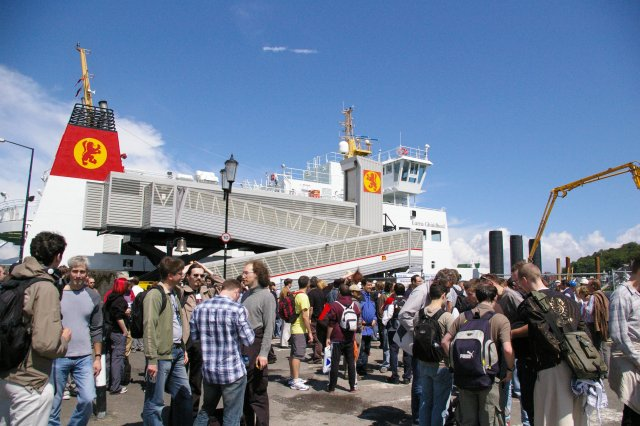
\includegraphics[width=5cm]{image200706/debconf7-daytrip.jpg}
\end{wrapfigure}

Rotheway $B$ND.$OEg$G!"FC$K$J$K$b$J$$$H$3$m$G$9!#$[$H$s$I$N7zJ*$OGd=PCf$G!"(B
$B:[H==j$N7zJ*$bGd$j$K=P$F$$$^$7$?!#:b@/$,$d$P$=$&$J46$8$G$9!#(B
$B7zB$J*$H$7$F$O!"652q$d!"%P%$%-%s%0$N?/N,$N:]$K@o$C$?>k$,$"$j$^$7$?$,!"=$I|Cf$G$7$+$b9);v$O;_$^$C$F$$$^$7$?!#(B
$B;3$N1|$X#1;~4V$[$IJb$/$H!"8P$,$"$j!"BgDq$N;22C<T$O$=$N8P$G%T%/%K%C%/$r$7$?$j!"%\!<%I(B
$B$K>h$C$FM7$s$G$$$?$h$&$G$9!#(B

\subsection{6$B7n(B21$BF|$NH/I=FbMF(B}
\subsubsection{Forking Debian every day}

GNU arch $B$G$$$+$K(B SELINUX$BHG$N(BDebian$B$N%]!<%F%#%s%0$r3Z$K$7$?$+!"$H$$$&%o!<(B
$B%/%U%m!<>R2p$N%;%C%7%g%s$N$O$:$G$7$?$,!"$$$m$$$m$H5;=QE*$J>c32$,$"$C$?$h(B
$B$&$G!"(B git $B$G(BDebian$B$N%Q%C%1!<%8$r%a%s%F%J%s%9$9$k$?$a$NJ}K!$r%G%b%s%9%H(B
$B%l!<%7%g%s$9$k%;%C%7%g%s$K5^n1JQ99$5$l$^$7$?!#%"%W%j%1!<%7%g%s$N3F<o5!G=(B
$B$r(BSCM$B$N%V%i%s%A$N5!G=$rMxMQ$7$F<BAu$7!"?7$7$$%P!<%8%g%s$,%j%j!<%9$5$l$F(B
$B$b(BSCM$B$N5!G=$,3hMQ$G$-$k!"$H$$$&OCBj$G$7$?!#(B

\subsubsection{Quality assurance activities for localization}

$B>.NS$5$s$,Ds0F$rDs=P$7DL$C$F$$$?$N$G$9$,!"$J$<$+(B Debconf7 $B$K;22C$7$J$+$C(B
$B$?$N$H!"Js9p!&<~CN!&BP:v$r2?$b9V$8$J$+$C$?$?$a3+:E$5$l$k$O$a$K$J$j$^$7$?!#(B

$B5^n1(B IRC $B$G8=CO$HF|K\$r7k$s$G>e@n$,%;%C%7%g%s$r9T$$$^$7$?!#%U%i%s%9!"%V(B
$B%i%8%k$J$I$N%A!<%`$G$NK]Lu$N?J$aJ}$d%D!<%k$N;H$$J}$K$D$$$F%G%#%9%+%C%7%g(B
$B%s$r9T$$$^$7$?!#%a!<%j%s%0%j%9%H$r%9%-%c%s$7$F$/$l$k%m%\%C%H%D!<%k$,$"(B
$B$j!"F|K\K]Lu%A!<%`8~$1$K;H$($k$h$&$KD4@0$7$F$/$l$k$H$N$3$H$G$7$?!#(B

\subsubsection{Debian ceilidh/Sun Drinks Reception}
\begin{wrapfigure}{r}{5cm}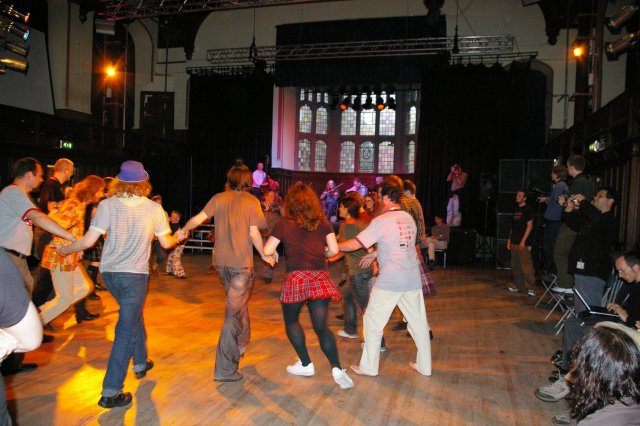
\includegraphics[width=5cm]{image200706/debconf7-dance.jpg}\end{wrapfigure}

Sun Microsystems $B$H(B Google $B$N%9%]%s%5$K$h$k%Q!<%F%#$G$7$?!#(BSun $B$,0{$_J*!"(B
Google $B$,%T%6$rDs6!$7$F$/$l$^$7$?!#$^$?!"%9%3%C%H%i%s%I$NL1MX$N1iAU2H$r8F(B
$B$S!"Bg%[!<%k$K=8$^$C$?%Q!<%F%#;22C<TC#$G%9%3%C%H%i%s%I$N%@%s%9$r3Z$7$_$^(B
$B$7$?!#(B

\subsection{6$B7n(B22$BF|$NH/I=FbMF(B}

\subsubsection{Derivatives Round Tables --- Debian$B$h$jGI@8$7$?%G%#%9%H%j%S%e!<%7%g%s(B}

Benjamin ``Mako'' Hill $B$,;J2q$rL3$a$k!"(BDebian $B$h$jGI@8$7$?%G%#%9%H%j%S%e!<(B
$B%7%g%s$N4X78<T$,=8$^$C$F$N%Q%M%k%;%C%7%g%s$G$7$?!#%Y%M%:%(%i$G3+H/$5$l$F(B
$B$$$k9q$N;Y1g$r<u$1$?%G%#%9%H%j%S%e!<%7%g%s!"%9%Z%$%s$N(B Extremadura$B!"(B
Debian Edu, Ubuntu$B$J$I$,;22C$7$F$-$F$$$^$7$?!#M=A[$I$*$jGrG.$7$^$7$?!#%G%#(B
$B%9%H%j%S%e!<%7%g%s$+$i$N%U%#!<%I%P%C%/$NItJ,$,LdBj$K$J$C$F$$$^$7$?!#(BBTS 
$B$N6&M-$J$I$b%H%T%C%/$K$J$C$F$$$^$7$?!#(B

\subsubsection{Proactive Bug Discovery}

  DPL$B$G$"$k!"(BSam Hocevar $B$N%;%C%7%g%s$G$7$?!#(B
\footnote{$B$3$N%;%C%7%g%s$N1Q8l$OLp?a$K$O$o$+$j$d$9(B
  $B$+$C$?!#(B}$B%=!<%9$rA4It%A%'%C%/$9$k$N$OHs>o$K%3%9%H$,9b$$$N$G!"%/%j%F%#%+(B
  $B%k$JItJ,$@$1$OA4It::FI$9$k$,!"$[$H$s$I$NItJ,$O!"%D!<%k$r;H$C$F5!3#E*$K(B
  $B%A%'%C%/$9$k$@$1$b$+$J$j$N$3$H$,$o$+$k$H$N$3$H$G$7$?!#(B

$B%=!<%9%3!<%I$r@55,I=8=$G%9%-%c%s$7$?$j!"(Bgoogle $B$N%3!<%I%5!<%A%(%s%8%s$G(B
  $B%A%'%C%/$7$?$j!"%3%s%Q%$%i!<$K%A%'%C%/$5$;$?$j$H$$$&ItJ,$K$D$$$F8l$C$F(B
  $B$/$l$^$7$?!#(B

\subsection{6$B7n(B23$BF|$NH/I=FbMF(B}

\subsubsection{debian-community.org}

  Debian$B%3%_%e%K%F%#$KBP$9$kLdBj0U<1$+$i!"(B
  \url{http://debian-community.org} $B$NDs0F%;%C%7%g%s$,9T$o$l$^$7$?!#(B
  Ubuntu$B%3%_%e%K%F%#$N;vNc$+$i$H$C$?$b$N$G$9!#(BDebian$B3+H/<T$K$J$j3hLv$9$k(B
  $B$^$G$N;~4V$,$+$+$k$N$,LdBj0U<1$H$J$C$F$$$^$9!#$=$NLdBj$r2r7h$9$k$Y$/!"(B
  debian-community.org$B$H$$$&%5%$%H$r:n$j!"(BDebian$B%3%_%e%K%F%#3hF0$9$k$H@k(B
  $B8@$7!"3hF0$7$F$$$k4V$O%a!<%k$NE>Aw$J$I$N%5!<%S%9$rDs6!$7$^$9!#3hF0$,0lDj(B
  $B4|4V;_$^$C$?$i!"$3$N3hF0%j%9%H$h$j30$5$l$^$9!#B>$K$b(Bplanet$B$d!"(Bwiki$B$J$I$N(B
  $BDs6!$r9T$&M=Dj$,$"$j$^$9!#(B

  $BLdBjE@$H$7$F$O!"$3$l$^$G$N%m!<%+%k%3%_%e%K%F%#$H$N@09g@-!"(Bdebian.org $BK\(B
  $BBN$b%3%_%e%K%F%#$G$"$k$3$H!"?7$7$$%3%_%e%K%F%#$r:n$C$F%I%i%$%V$7$F$$$/(B
  $B$@$1$NL%NO$,$=$3$K$"$k$+$J$I$,OC$79g$o$l$^$7$?!#(B

\subsubsection{WTFM, again: Write The Fine Manual page}

Debian package $B$GHRI[$5$l$F$$$k%W%m%0%i%`$K$O(B man $B$,IUB0$7$F$$$J$$$H(B
$B$$$1$J$$$H$$$&$3$H$,(B Debian Policy $B$G7h$^$C$F$$$k$,!"(Bnroff $B7A<0$N(B man
$B$O;~BeCY$l$G$9!#(Bman $B$@$1$G$J$/!"$"$i$f$k%U%)!<%^%C%H$KBP1~$7$?%I%-%e%a%s%H$r(B
$BMF0W$K:n@.$9$k$K$O$I$&$7$?$$$$$N$+OC$7!"(BDocBook XML $B$r;H$C$?>l9g$N4JC1$J(B
$B%A%e!<%H%j%"%k$r9T$$$^$7$?!#(B
$B$^$?!"(Bman $B$O$"$k$,!"(BLinux $B$N(B man $B$G$O$/!"(BUnix $B$N(B man $B$@$C$?$j$9$k$3$H$,(B
$B$"$k$N$G!"%f!<%6!<$K(B man $B$rDs6!$9$k:]$KCm0U$9$Y$-;v$J$I$rOC$7$^$7$?!#(B

Debian package $B$GHRI[$5$l$F$$$k%W%m%0%i%`$K$O(B man $B$,IUB0$7$F$$$J$$$H$$$1(B
$B$J$$$H$$$&$3$H$,(B Debian Policy $B$G7h$^$C$F$$$k$,!"(Bnorff $B7A<0$N(B man $B$O;~Be(B
$BCY$l$G$9!#(Bman $B$@$1$G$J$/!"$"$i$f$k%U%)!<%^%C%H$KBP1~$7$?%I%-%e%a%s%H$rMF(B
$B0W$K:n@.$9$k$K$O$I$&$7$?$$$$$N$+OC$7!"(BDocBook XML $B$r;H$C$?>l9g$N4JC1$J(B
$B%A%e!<%H%j%"%k$r9T$$$^$7$?!#$^$?!"(Bman $B$O$"$k$,!"(BLinux $B$N(B man $B$G$O$/!"(B
Unix $B$N(B man $B$@$C$?$j$9$k$3$H$,$"$k$N$G!"%f!<%6!<$K(B man $B$rDs6!$9$k:]$K=q(B
$B$$$F$"$kFbMF$,K\Ev$KBEEv$J$N$+3NG'$9$Y$-;v$J$I$rOC$7$^$7$?!#(B
 
\subsubsection{pbuilder talk}

$B>e@n(B $B=c0l(B $B$,(Bpbuilder, cowbuilder, qemubuilder $B$K$D$$$F$N5DO@$r9T$$$^$7$?!#(B
pbuilder $B$rMxMQ$7$F$$$k%f!<%6$OHs>o$KB?$$$,!"(Bqemubuilder $B$NMxMQ<T$O?t?M(B
$B$b$$$J$+$C$?$H$$$&$3$H$,$o$+$j$^$7$?!#$^$?!"%^%K%e%"%k$NB8:_$r$7$i$J$$!!(B
$B?M$,B??t$$$^$7$?!#(B

\subsubsection{Lightning Talks}

$B%i%$%H%K%s%0%H!<%/$O<c43%*!<%,%J%$%:$K<:GT$7$F$*$j!":G=i7W2h$7$F$$$?%a%s(B
$B%P!<$,$"$^$j$$$J$+$C$?$?$a!"9%$-$J?M$,9%$-$J$3$H$r8l$k$H$$$&2q$K$J$C$F$7(B
$B$^$$$^$7$?!#(B

\subsubsection{Closing ceremony}

$B:G8e$N$7$a$N0';"$,$J$5$l!"%9%]%s%5!<$K46<U$7$?$j$7$^$7$?!#(B

\subsection{$B9V1i0J30$N$G$-$4$H(B}

\subsubsection{apt-listbugs $B4XO"$NF$O@(B}

Don Armstrong $B$,$-$F$*$j!"(Bbugs.debian.org $B$N(B SOAP$B%$%s%?%U%'!<%9$r3HD%$7(B
$B$?!"$H$$$$$^$7$?!#(Bapt-listbugs $B$N<BAu$rJQ99$7!"(BSOAP$B%$%s%?%U%'!<%9$rMxMQ(B
$B$9$k$h$&$K$7!"8=:_%5!<%PB&$G@8@.$7$F$$$k%$%s%G%C%/%9%U%!%$%k$,!"$b$&I,MW(B
$B$J$$$h$&$K$7$^$7$?!#8=CO$G(B SOAP $B%$%s%?%U%'!<%9$N%G%P%C%0$r<B;\$7!"<BMQ$K(B
$B$J$k$h$&$K$7$^$7$?!#(B

$B$^$?!"(B debian-changelog-mode $B$K0JA0%Q%C%A$r$*$/$C$F$/$l$?(B Luca Capello 
$B$H(B BTS $B$N(B HTML $B$r%Q!<%9$7$F$$$k$+$i$@$5$$$s$@$h!"$H$$$&OC$r$7$?$i!"(B SOAP 
$B$r(B emacs $B$+$i$D$+$&$N$O$$$d$J$N$G!"(Bapt-listbugs $B$r;H$*$&$H$$$&OC$K$J$j!"(B 
apt-listbugs list $B%3%^%s%I$r3HD%$7$F<BAu$9$k$3$H$K$J$j$^$7$?!#$7$+$7!"$=(B
$B$l$,<BAu$5$l$k$^$($K!"(Bvim $B$N%a%s%F%J(B Stefano Zacchioli $B$,$=$NOC$r$&$7$m(B
$B$GJ9$$$F$$$F!"$=$N>l$G(Bvim $BMQ$N(B debian/changelog $B$G$N(B closes: $BJd40%3!<%I$,(B
$B<BAu$5$l$F$7$^$$$^$7$?!#(B

\subsubsection{QEMU $B4XO"$NF$O@(B}

$B>e@n$O(B qemu$B!"(Bqemubuilder $B4XO"$GG.$/5DO@$7$F$^$o$j$^$7$?!#(B

Thiemo Seufer (QEMU mips $B%]!<%H$N%a%s%F%J$G(B QEMU $B$N%3%_%C%?!"$*$h$S(B
Debian $B$N(B MIPS $B%]!<%H$N%a%s%F%J!K$H5DO@$7$^$7$?!#(Bchroot $BFbIt$G$N(B qemu
user emulation $B$r$$$+$K(B static link $B$r$7$J$$$G<B;\$9$k$N$+!"$H$$$&E@$K$D(B
$B$$$F5DO@$7!"4D6-JQ?t$rDj5A$9$kI,MW$,$"$k$M!"$H$$$&$3$H$G9g0U$7$^$7$?!#(B

$BM<?)$N;~4V$G(B Ottavio $B$H5DO@$7!"(Bqemubuilder $B$N@_7W$H!"(Bqemu system
emulation $B$G$O$J$/(B qemu user emulation $B$G$N<BAu$K$D$$$F5DO@$7$^$7$?!#(B


\subsubsection{$BLp?a!_(Bgrisu}

apt$B$K(Bi18n$B5!G=$,%^!<%8$5$l$?$N$K$^$@%5!<%PB&$N%$%s%U%i$N@0Hw$,9T$o$l$F$$$^(B
$B$;$s!#Lp?a$O(BDDTP$B$NC4Ev<T$N(B Grisu $B$H(B DDTP $B$NE83+$K$D$$$F5DO@$7$F$$$k$h$&$G(B
$B$7$?!#$J$s$i$+$N@.2L$,$G$k$H$h$$$G$9$M!#(B

\subsection{$BMhG/$N(B Debconf}

$BMhG/$N(B Debconf $B$O%"%k%<%s%A%s$G(B8$B7n$K9T$o$l$^$9!#F|K\$O2F$G$9$,!"%"%k%<%s(B
$B%A%s$OE_$G$9!#E_4|9g=I$K$J$k$H;W$$$^$9$N$G!"5$9g$$$r$$$l$F$$$+$J$$$H!"$R(B
$B$I$$$3$H$K$J$k$+$b$7$l$^$;$s!#5$$rIU$1$^$7$g$&!#(B

\dancersection{Debconf $B;22CJs9p(B}{$B4d>>(B $B?.MN(B}
\label{sec:debconfreportsummary}
\index{Debconf2007}
\index{Debconf}

\subsection{Debconf$B$H$O(B}

  2007$BG/EY$N(B Debconf $B$O(B 6$B7n(B13$BF|$+$i(B6$B7n(B23$BF|$^$G!"1Q9q%9%3%C%H%i%s%I$N%(%8(B
$B%s%P%i$G9T$o$l$^$7$?!#F|K\$+$i$O!">e@n(B $B=c0l!"Lp?a(B $B9,<#!"4d>>(B $B?.MN$,;22C(B
$B$7$^$7$?!#(B

\subsubsection{Debconf$B$NNr;K!&7P0^(B}

Debian Conference \url{http://debconf7.debconf.org/} $B$O(B Debian 
$B$N3+H/<T$?$A$,0lF1$K2p$9$k%$%Y%s%H$G$9!#DL>o4i$r$"$o$;$k$3$H$N$J$$%a%s%P!<(B
$B$?$A$,0lF1$K2p$7M'9%$r?<$a!"5;=QE*$J5DO@$r@o$o$;$^$9!#2a5n$N3+:EMzNr$r8+(B
$B$F$_$k$H(B\tbref{tab:debconflist}$B$N$h$&$K$J$j$^$9!#(B

\begin{table}[H]
\caption{$BNrBe$N(BDebconf$B;22C<T?d0\(B}
\label{tab:debconflist}
 \begin{center}
 {\footnotesize
 \begin{tabular}{|c|c|c|r|}
 \hline
 $BG/(B & $BL>A0(B & $B>l=j(B & $B;22C?M?t(B \\
 \hline
 2000 & debconf 0 &$B%U%i%s%9(B $B%\%k%I!<(B & \\
 2001 & debconf 1 &$B%U%i%s%9(B $B%\%k%I!<(B & \\
 2002 & debconf 2 &$B%+%J%@(B $B%H%m%s%H(B & 90$BL>(B \\
 2003 & debconf 3 &$B%N%k%&%'!<(B $B%*%9%m(B & 140$BL>(B \\
 2004 & debconf 4 &$B%V%i%8%k(B $B%]%k%H%"%l%0%l(B &  150$BL>(B \\
 2005 & debconf 5 &$B%U%#%s%i%s%I(B $B%X%k%7%s%-(B & 200$BL>(B \\
 2006 & debconf 6 &$B%a%-%7%3(B $B%*%"%9%?%Z%C%/(B & 300$BL>(B \\
 2007 & debconf 7 &$B1Q9q%9%3%C%H%i%s%I(B $B%(%8%s%P%i(B & $BLs(B400$BL>(B \\
 \hline
 \end{tabular}
 }
 \end{center}
\end{table}

\subsubsection{Debconf 2007}

2007$BG/EY$N(BDebconf$B$N2q>l$O%(%8%s%P%iBg3X$N3X@82q4[(B Teviot $B$r3hMQ$7$^$7$?!#(B
$B@lMQ$N%M%C%H%o!<%/2s@~$r$O$j$a$0$i$;!"L5@~(BLAN$B%M%C%H%o!<%/$b$O$j$a$0$i$;(B
$B$^$7$?!#(B

$B$^$?!"(BTeviot $B$O(B $BLk(B10$B;~$KJD:?$9$kI,MW$,$"$C$?$N$G!"Lk$N2q>l(B(night venue) 
$B$H$$$&$b$N$b=`Hw$5$l$^$7$?!"8=:_Gd$jJ*7o$H$J$C$F$$$k;H$o$l$F$$$J$$652q$r(B
$B;HMQ$7!"%O%C%/%i%\$K$7$^$7$?!#%Q%$%W%*%k%,%s$J$I$,$"$j!"Iw>p$,$"$j$^$7$?!#(B
$B%Q%$%W%*%k%,%s$O$b$H$b$H2u$l$F$$$?$N$G$9$,!"(BDebconf $B$N2q4|Cf$K=$I|$5$l!"(B
$B1iAU2q$,:E$5$l$^$7$?!#(B

$B=IGq$O2q>l$+$iELJb(B5$BJ,DxEY$K0LCV$9$k(B Budget Backpackers $B$H(B Cowgate hostel 
$B$H$$$&Fs$D$N%[%9%F%k$KJ,;6$7$F9T$$$^$7$?!#(B

\subsection{$B%9%3%C%H%i%s%I(B/$B%(%8%s%P%i(B}

\subsubsection{$B9T$-J}(B}
  $BF|K\$+$i%(%8%s%P%i$^$G$O!"D>9TJX$,$"$j$^$;$s!#%Q%j7PM3$+!"%m%s%I%s7PM3Ey$G0l2s(B
  $B%H%i%s%8%C%H$,I,MW$G$9!#5wN%$OLs(B10000km$B!#Ht9T;~4V$OLs(B14$B;~4V$+$+$j$^$9!#(B
  $B>e@n!"4d>>AH$O%Q%j$N(B $B%7%c%k%k!&%I!&%4!<%k9q:]6u9A7PM3!"Lp?a$O%R!<%9%m!<7PM3$GF~9q$7$^$7$?!#(B

\subsubsection{$B2q>l(B}

\begin{wrapfigure}{r}{11cm}
  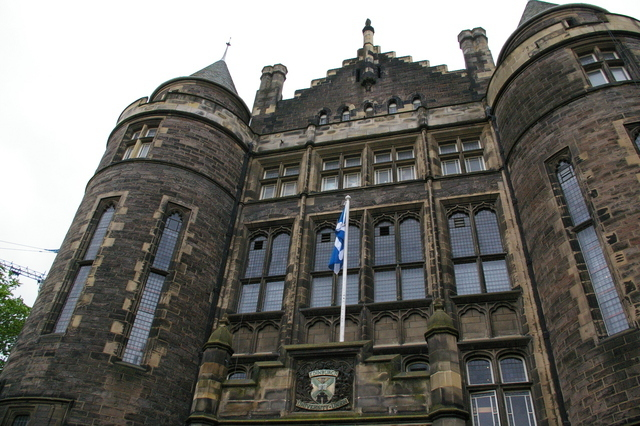
\includegraphics[width=5cm]{image200706/teviot.jpg}
  
\includegraphics[width=5cm]{image200706/debconf7-debian.jpg}
\end{wrapfigure}
  $B2q>l$O!"%(%8%s%P%iBg3X$N7zJ*$N0lIt$G$"$k(B Teviot $B$H$$$&L>A0$N(B
  $B7zJ*$r<Z$j@Z$j!"3+:E$5$l$^$7$?!#(B

 $B;22C<T$O$U$?$D$N%[%F%k$KJ,;6$7$F=IGq$7$F$$$?$N$G$9$,!"$=$l$i$N%[%F%k$+$iJb$$$F(B
  10 $BJ,$[$I$N$H$3$m$K$"$j$^$9!#(B
\\

\begin{itemize}
  \item Upper Talk Room: 	$B%a%$%sMQ!#(B250$B?M$[$IF~$k$3$H$,$G$-$^$9!#(B\\
	\begin{minipage}{0.4\hsize}
	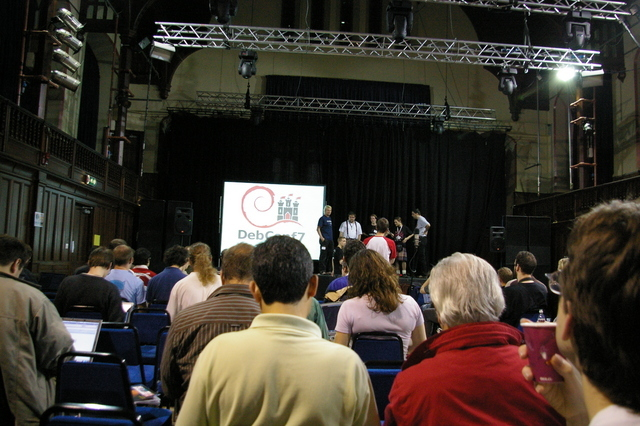
\includegraphics[width=0.8\hsize]{image200706/debconf7-upper-talk.jpg}
	\end{minipage}
  \item Basement Talk Room\\
	$B%5%VMQ!#(B50$B?M$[$IF~$k$3$H$,$G$-$^$9!#(B
  \item Lower BoF Room\\
	BOF $BMQ!#(B20$B?M$[$IF~$k$3$H$,$G$-$^$9!#(B
  \item Upper BoF Room\\
	BOF $BMQ!#(B20$B?M$[$IF~$k$3$H$,$G$-$^$9!#(B
  \item Hacklab 1: 	$B%O%C%/MQ!#(B\\
	\begin{minipage}{0.4\hsize}
	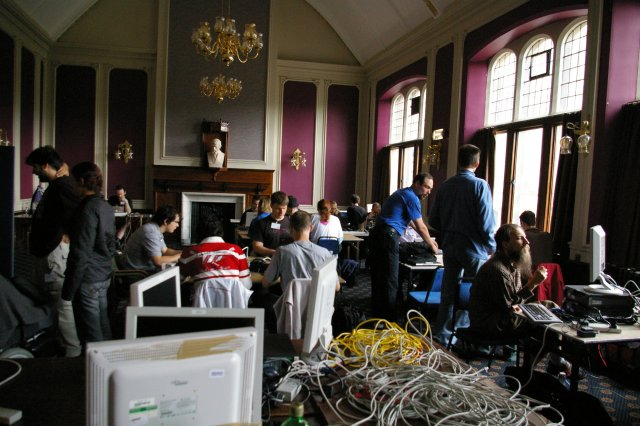
\includegraphics[width=0.8\hsize]{image200706/debconf7-hacklab00.jpg}
	\end{minipage}

  \item Hacklab 2: $B%O%C%/MQ!#DL>o$O%P!<$i$7$$$G$9!#(B\\
	\begin{minipage}{0.4\hsize}
	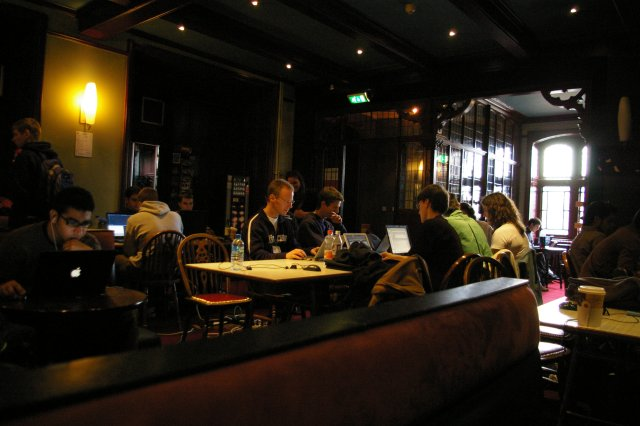
\includegraphics[width=0.8\hsize]{image200706/debconf7-hacklab01.jpg}
	\end{minipage}
  \item Night venue:
	$BGQTR$H2=$7$?652q!#%Q%$%W%*%k%,%s$,$"$C$?$j$7$^$9!#(B
	$BLk$N(B22$B;~0J9_$O(B Teviot $B$r;H$&$3$H$,$G$-$J$$$N$G(B
	$B$3$3$r<Z$j$F$_$s$J$G%O%C%/$7$?$j!"OC$79g$C$?$j$7$^$7$?!#(B
\\
     	\begin{minipage}{0.4\hsize}
     	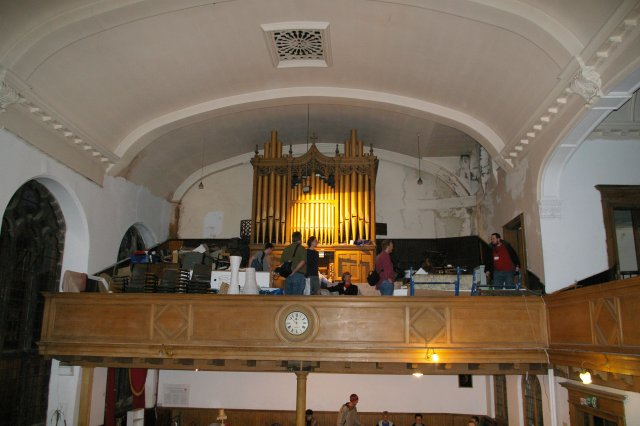
\includegraphics[width=0.8\hsize]{image200706/debconf7-elsewhere.jpg}
     	\end{minipage}
     	\begin{minipage}{0.4\hsize}
     	\end{minipage}
\end{itemize} 

\subsection{$B%9%1%8%e!<%k(B}

\begin{wrapfigure}{r}{8cm}
 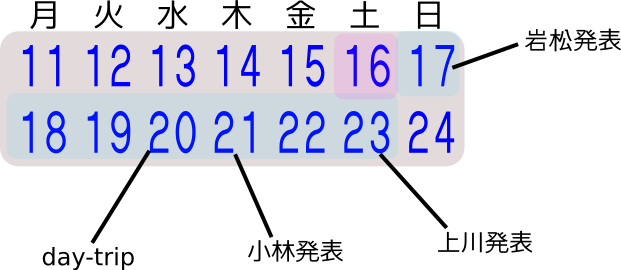
\includegraphics[width=1\hsize]{image200707/schedule.png}
\caption{$BA4BN%9%1%8%e!<%k(B}
\label{fig:schedule}
\end{wrapfigure}
16$BF|$N(BDebian Day $B$G(B Debian Conference $B$O3+;O$7!"(B23$BF|$^$GKhF|$$$m$$$m$JM=(B
$BDj$,$/$^$l$F$$$^$7$?!#(B
$B#2#0F|$@$1$O%+%s%U%!%l%s%9;22C<T$G(B day-trip $B$r<B;\$7$^$7$?!#(B

\begin{wrapfigure}{r}{8cm}
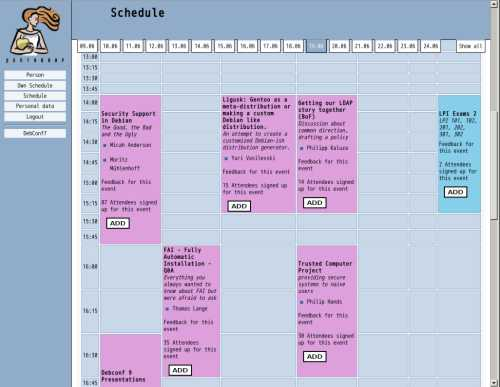
\includegraphics[width=8cm]{image200707/penta.png}
\caption{pentabarf $B2hLL(B}
\label{fig:penta}
\end{wrapfigure}
 $B%9%1%8%e!<%k$O(B ruby-on-rails $B$G<BAu$5$l$?(B 
pentabarf $B%7%9%F%`(B(\fgref{fig:penta})$B$G4IM}$7$F$$$^$7$?!#(B
$B%9%1%8%e!<%k$K$O(B
$B?o;~JQ99$,$+$+$j!"(BIRC bot $B$G$NDLCN$,$J$+$C$?$iC/$b>u67$K$*$$$D$1$J$+$C(B
 $B$?$G$7$g$&!#(B


\subsection{$B<g$H$J$C$?F$O@(B}

\subsubsection{$BAH9~$_7O$K$D$$$F$NGrG.$7$?5DO@(B}

ARM EABI $B$NF3F~$,Bg$-$J%H%T%C%/$G$9!#F|K\$+$i(B SuperH $B$N(B
$BOCBj$b$b$C$F$$$-$^$7$?!#%^%$%s%I%7%'%"$,$*$*$-$/$J$C$F$$$k$h$&$G$9!#(B
$B$^$?!"AH9~4X78$NBP1~$r(B Debian $B$G9T$&$?$a$N5DO@$b9T$o$l$^$7$?!#(B
New DPL $B$N(B Sam Hocevar $B$,AH9~$_4X78$K6=L#$,$"$k$h$&$J$N$G!"(B
$B$$$^$^$GDdBZ$7$F$$$?AH9~$_4X78$K$h$k@.2L$N%^!<%8$,2CB.$9$k$+$b$7$l$^$;$s!#(B

\subsubsection{$B%P!<%8%g%s4IM}%7%9%F%`$H%=!<%9%3!<%I4IM}$NOC(B}

git $B$NMxMQJ}K!$N%A%e!<%H%j%"%k$d!"(Barch $B$rNc$K$H$C$F$N(BDebian$B%G%#%9%H%j%S%e!<(B
$B%7%g%s$N%U%)!<%/$r%a%s%F%J%s%9$9$k$?$a$N%=!<%9%3!<%I4IM}$N$d$j$+$?$K$D$$(B
$B$F$N>R2p$,$"$j$^$7$?!#(Bgit $B$J$I$NIa5Z$K$h$jJ,;6(BSCM$B$,Ia5Z$7!"%=!<%9%3!<%I(B
$B$N4IM}$N%o!<%/%U%m!<$K1F6A$7$F$*$j!":F9M$,I,MW$@$H$$$&IwD,$,8+$i$l$^$7$?!#(B

$BFC$K(B ubuntu $B$G%=!<%9%3!<%I4IM}$r8+D>$7$F$*$j!"(Bbazaar$B$rCf?4$H$7$F%V%i%s%A(B
$B$r(Bdpatch$B$N%Q%C%A%U%!%$%k$KJQ49$7$?$j$9$k%D!<%k$J$I$N%$%s%U%i$,$H$H$N$$;O(B
$B$a$F$$$k$H$$$&$3$H$,Bg$-$$$h$&$G$9!#(B

\subsubsection{$BK]Lu$K$D$$$F$N5DO@(B}

$BK]Lu4X78$NOC$,KhF|9T$o$l$^$7$?!#KhF|5DO@$r=E$M!"5DO@$7$?7k2L$rKhHU%I%-%e%a%s%H(B
$B$r=$@5$7$F$$$^$7$?!#(B
$B$^$?!";~4|%j%j!<%9$N(B lenny $B$^$G$K!"K]Lu$N%$%s%U%i$d%I%-%e%a%s%H@0M}(B
$B$r9T$&M=Dj$@$=$&$G$9!#(B

$B>.NS$5$s$NK]Lu4X78$N%$%s%U%i$K4X$9$k%;%C%7%g%s$,$"$C$?$N$G$9$,!"(B
$B>.NS$5$s$,Mh$i$l$J$+$C$?$N$G!">e@n$5$s$,BeM}$G(B BOF $B$r9T$$$^$7$?!#(B
$B3F9q$G;HMQ$5$l$F$$$k%D!<%k$N>R2p$J$I$,$"$j$^$7$?!#F|K\$G$bF3F~$r8!F$(B
$B$r$9$kI,MW$,$"$j$=$&$G$9!#(B

\subsubsection{Daytrip}


\begin{wrapfigure}{r}{5cm}
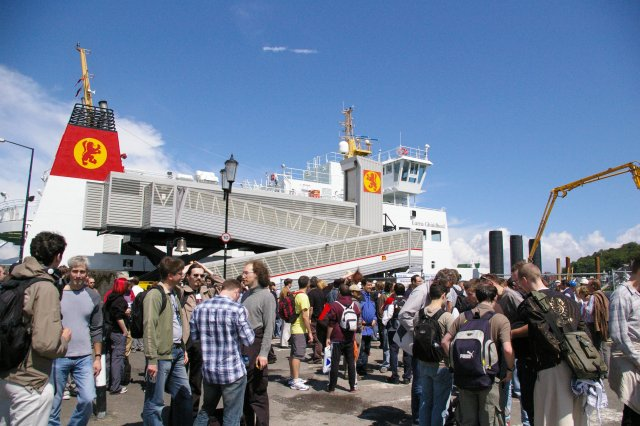
\includegraphics[width=5cm]{image200706/debconf7-daytrip.jpg}
\end{wrapfigure}

Debconf $B$G$O0lF|!";22C<T$GN99T$r$9$k$H$$$&%$%Y%s%H$,$"$j$^$9!#:#2s$N(B
Debconf$B$G$O(B Rotheway (Bute$BEg(B) $B$G$^$C$?$j$H%T%/%K%C%/$r$7$^$7$?!#(BRotheway 
$B$X$N0\F0$O!"(BEdinburgh $B$+$i(B Glasgow $B$XEE<V$G0\F0$7!"(BGlasgow $B$+$i$5$i$KEE(B
$B<V$G(B Wemyss Bay $B$X0\F0$7$^$9!#(BWemyss Bay $B$O(B Rotheway $B9T$-@lMQ$N=.Ce$->l(B
$B$G!"$=$3$+$iA%$K>h$C$F(B Rotheway $B$K0\F0$7$^$7$?!#(B

Rotheway $B$ND.$OEg$G!"FC$K$J$K$b$J$$$H$3$m$G$9!#$[$H$s$I$N7zJ*$OGd=PCf$G!"(B
$B:[H==j$N7zJ*$bGd$j$K=P$F$$$^$7$?!#:b@/$,$d$P$=$&$J46$8$G$9!#(B
$B7zB$J*$H$7$F$O!"652q$d!"%P%$%-%s%0$N?/N,$N:]$K@o$C$?>k$,$"$j$^$7$?$,!"=$I|Cf$G$7$+$b9);v$O;_$^$C$F$$$^$7$?!#(B
$B;3$N1|$X#1;~4V$[$IJb$/$H!"8P$,$"$j!"BgDq$N;22C<T$O$=$N8P$G%T%/%K%C%/$r$7$?$j!"%\!<%I(B
$B$K>h$C$FM7$s$G$$$?$h$&$G$9!#(B

\dancersection{$B>-Mh$N(B Debconf }{$B>e@n(B $B=c0l(B}
\label{sec:debconfplanning}
\index{Debconf}


Debconf $B$OMhG/$O%"%k%<%s%A%s$G$9$,!">-MhE*$K$OF|K\$G$b3+:E$G$-$k$H$h$$$G(B
$B$9$M!#(B
$B$^$?!"(BDebconf$B$N3+:EFbMF$r$$$+$KM-1W$K;H$($k$+!"9M$($F$_$^$7$g$&!#(B


\subsection{$B@.2L$N3hMQ(B}

Debian Conference$B$K$OJ#?t$NB&LL$,$"$j$^$9!#@.2L$O$I$&$d$C$F$G$-$k$N$G$7$g(B
$B$&$+!#(B

\begin{table}[H]
\caption{$B;22C$N@.2L(B}
\label{tab:framework}
\begin{center}
{\LARGE
  \begin{tabularx}{\hsize}{|c|X|X|}
 \hline
 & $B;22C$7$?>l9g(B & $B;22C$7$J$+$C$?>l9g(B \\
 \hline
 $B%3!<%I(B	& $B9g=I$7$F%3!<%I$,$+$1$k(B &  \\
 \hline
 $BJ8=q2=(B	& $B9g=I$7$FJ8=q$,$+$1$k(B&  \\
 \hline
 $B5DO@(B 	& $BD>@\5DO@$G$-$k(B &  \\
 \hline
 $BH/I=(B 	& $B%;%C%7%g%s$K;22C$7$FH/I=$G$-!"H/I=$r$-$/$3$H$,$G$-$k!#(B &  \\
 \hline
&&\\
 \hline
&&\\
 \hline
 \end{tabularx}
}
\end{center} 
\end{table}

$B$3$l$rF'$^$($k$H!"3+:E<+BN$O=EMW$G$9$,!";22C$K$O$*$h$S$^$;$s!#(B
$B$"$J$?$b;22C$7$?$/$J$C$F$-$?$N$G$O$J$$$G$9$+!)(B

\subsection{$BF|K\3+:E(B}

Debian Developer $B$NCf$G$O(B Debian Conference $B$rF|K\$G3+:E$7$?$$$H;W$C$F$$(B
$B$k%a%s%P!<$,$$$^$9!#F|K\$G3+:E$9$k$H$9$l$P!"F|K\$G3+:E$9$k$?$a$N%A!<%`$,(B
$BI,MW$G$9!#F|K\$G?tEY%$%Y%s%H$r1?1D$7$F1_3j$K$9$9$a$i$l$k$h$&$K$7$F$*$/$3(B
$B$H$bI,MW$G$7$g$&!#(B

$BF|K\$G$N(BDebconf$B$N8!F$$N?JD=$K$D$$$F$O(B
\url{http://wiki.debian.org/DebConfInJapan}
$B$G@0M}$5$l$F$$$^$9!#(B

\begin{table}[H]
\caption{2005$BG/$K<B;\$7$?3F<o6u9A$KE~Ce$9$k$^$G$N%3%9%HI>2ANc(B}
\label{tab:framework}
\begin{center}
{\LARGE
  \begin{tabularx}{\hsize}{|c|X|X|X|}
 \hline
 & $B%U%i%s%9(B & $B%"%a%j%+(B & $BFnJF(B \\
 \hline
$B@.ED(B & 828 & 809 & 1600 \\
$B@i:P(B &980 & 1197 &2121 \\
$B4X@>(B &736 & 809 &1718 \\
$B2-Fl(B &1485 & 1197 &4307 \\
 \hline
 \end{tabularx}
}
\end{center} 
\end{table}

\dancersection{OSC-Kansai $B;22CJs9p(B}{$B;32<(B $BB:Li(B}
\label{sec:osckansai2007}
\index{Open Source Conference@Open Source Conference}
\index{$B$+$s$5$$$G$S$"$s(B@$B4X@>(BDebian$BJY6/2q(B}
\index{debianjp@Debian JP}

\subsection{$B3+:E35MW(B}
$B4X@>(B Debian $BJY6/2q$O!"(B7$B7n(B20,21$BF|$K5~ET%3%s%T%e!<%?3X1!$G3+:E$5$l$?%*!<%W(B
$B%s%=!<%9%+%s%U%!%l%s%9(B2007 Kansai$B!J0J2<!"(BOSC Kansai$B!K(B $B$K(B $B5~ET$J$i$S$K4X(B
$B@>COJ}$G$b(B Debian $B$N%W%l%<%s%9$r8~>e$5$;$k$?$a;22C$7$^$7$?!#(B
$B$^$?!"(B7$B7n$N4X@>(BDebian $BJY6/2q$H$7$F$N0LCV(B
$BIU$1$G!"Bh(B4$B2s(B $B4X@>(BDebian $BJY6/2q$H$7$F$$$^$9!#(B

1$BF|L\$O!"GX9-B2$NJ}$,B?$$$H;W$C$F$$$^$7$?$,!"$=$3$^$GB?$/$J$/!"5~ET%3%s%T%e!<(B
$B%?3X1!$N@8EL$5$s$,B?$+$C$?$G$9!#(B

2$BF|L\$O!"4X@>(B Debian $BJY6/2q$+$i%V!<%9$X$N6(NO$7$FD:$$$?J}$,B?$+$C(B
$B$?$N$G!"F~8}$N??$C@5LL$G$"$k5~ET%3%s%T%e!<%?3X1!$N%7%s%\%k$G$b$"$k3,CJ$N(B
$B2<$K%V!<%9$r0\F0$7!"$5$i$KB?$/$NJ}$,%V!<%9$KB-$r1?$s$G$$$?$@$-$^$7$?!#(B

\begin{figure}[H]
 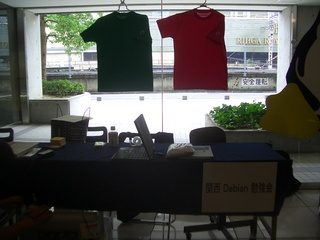
\includegraphics[width=0.5\hsize]{image200708/0720booth.jpg}
 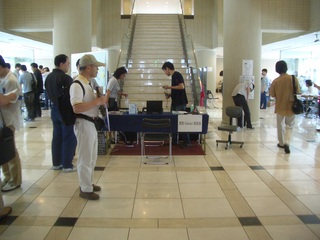
\includegraphics[width=0.5\hsize]{image200708/0721booth.jpg}
\caption{$BE8<(Iw7J(B}
\label{fig:osctenjifukei}
\end{figure}

\subsection{$B%;%C%7%g%s(B}

$B:#2s!"%;%C%7%g%s$O(B13:00-13:45$B$H8@$&(B45$BJ,4V$7$+$"$j$^$;$s$G$7$?$,!"(B25$B?M$N(B
$BJ}$K;22C$7$FD:$-$^$7$?!#0J2<$NFbMF$K$D$$$F9T$$$^$7$?!#(B

\begin{enumerate}
 \item $B4X@>(B Debian $BJY6/2q$H$O!!;32<(B $BB:Li(B
 \item Debian.org / Debian JP / $B4X@>(B Debian $BJY6/2q$N4X78!!Lp?a(B $B9,<#(B
 \item Debconf 7 $B%_%KJs9p(B + Debconf $BF|K\3+:E$K$D$$$F!#!!Lp?a(B $B9,<#(B
\end{enumerate}

$B9V;U$O!"(BDebianJP$B2q0w$G$"$j!"4X@>(B Debian $BJY6/2q$K$D$$$FF0$$$F$$$k;d$HLp?a$5$s(B
$B$,9T$$$^$7$?!#(B

$B;d$N%;%C%7%g%s$O!"4X@>(B Debian $BJY6/2q$H$O$H$$$&Bj$G!"(BOSC Kansai$B$K;22C$7$F(B
$BD:$$$F$kJ}$K$b!"4X@>(B Debian $BJY6/2q$K:#8e;22C$7$FD:$1$k$h$&$K!";22C$70W$$(B
$BJY6/2q$r%"%T!<%k$7$?$+$C$?$N$G!"$$$/$D$+$N>P$$$rF~$l$F@bL@$7$^$7$?!#(B
$BBh(B3$B2s$G$N!V%V%k!<%9%^%s!W$5$s$N%U%!%$%"!<%&%)!<%k%U%j!<%@%`$N2hA|$d!"$J$<!"(B
$B4X@>(B Debian $BJY6/2q$N%7%s%\%k$,!V$[$C$1!W$G$"$k$N$+$r@bL@$9$k$H!"2q>l$+$i(B
$B$O>P$$$,5/$3$j$^$7$?!#(B

$BLp?a$5$s$N%;%C%7%g%s$O!":#$^$G!"(BDebian JP$B$H4X@>(B Debian $BJY6/2q$H$N4X78$K(B
$B$D$$$F=R$Y$k5!2q$,$J$+$C$?$N$G!";22C$7$FD:$$$?J}$K$O!"4X78$J$I$,M}2r$7$F(B
$BD:$1$^$7$?!#6qBNE*$K$O!"(B8$B7n(B12$BF|!JF|!K$K?@8M8&5f3X1`ET;T$G9T$o$l$?Bh(B4$B2s(B
$B4X@>(B Debian $BJY6/2q$G!";22CHq$K$D$$$F5DO@$7$?:]$K!"(BOSC Kansai$B$GD0$$$F$$$?(B
$B$?$a!"J,$+$j0W$+$C$?$H$*$7$c$C$FD:$-$^$7$?!#$?$@!":#$^$G4X@>(B Debian $BJY(B
$B6/2q$G$O!"$3$N$h$&$J4X78$K$D$$$F=R$Y$k5!2q$,>/$J$+$C$?$?$a!":#8e5!2q$rA}(B
$B$d$9I,MW$,$"$k$H;W$$$^$7$?!#(B
$B$^$?!"(BDebconf$B$K$D$$$F$O!"Lp?a$5$s$N(B Debconf $B$G<j$KF~$l$?$*EZ;:$r7JIJ$K$7(B
$B$F!"%/%$%:$r9T$$$^$7$?!#%/%$%:7A<0$G$7$?$,!"<j$r$"$2$FD:$1$kJ}$,>/$J$+$C(B
$B$?$N$,;DG0$G$7$?!#4X@>9q:]6u9A$b$"$j$^$9$N$G!"4X@>$G3+:E=PMh$=$&$J(B
$B>l=j$r65$($F$$$?$@$1$k$h$&$KF/$-$+$1$^$7$?!#(B

\subsection{$B%V!<%94k2h(B}

\subsubsection{$B%j%"%k7G<(HD(B}

$B:#2s!"4X@>(B Debian $BJY6/2q$G$O!"$_$J$5$s$N0U8+$rIUd5;f$K=q$$$F$b$i$$!"(B
Debian $B$K$D$$$F$N0U8+$r=q$$$F$b$i$$$^$7$?!#(B

\begin{figure}[H]
\begin{center}
  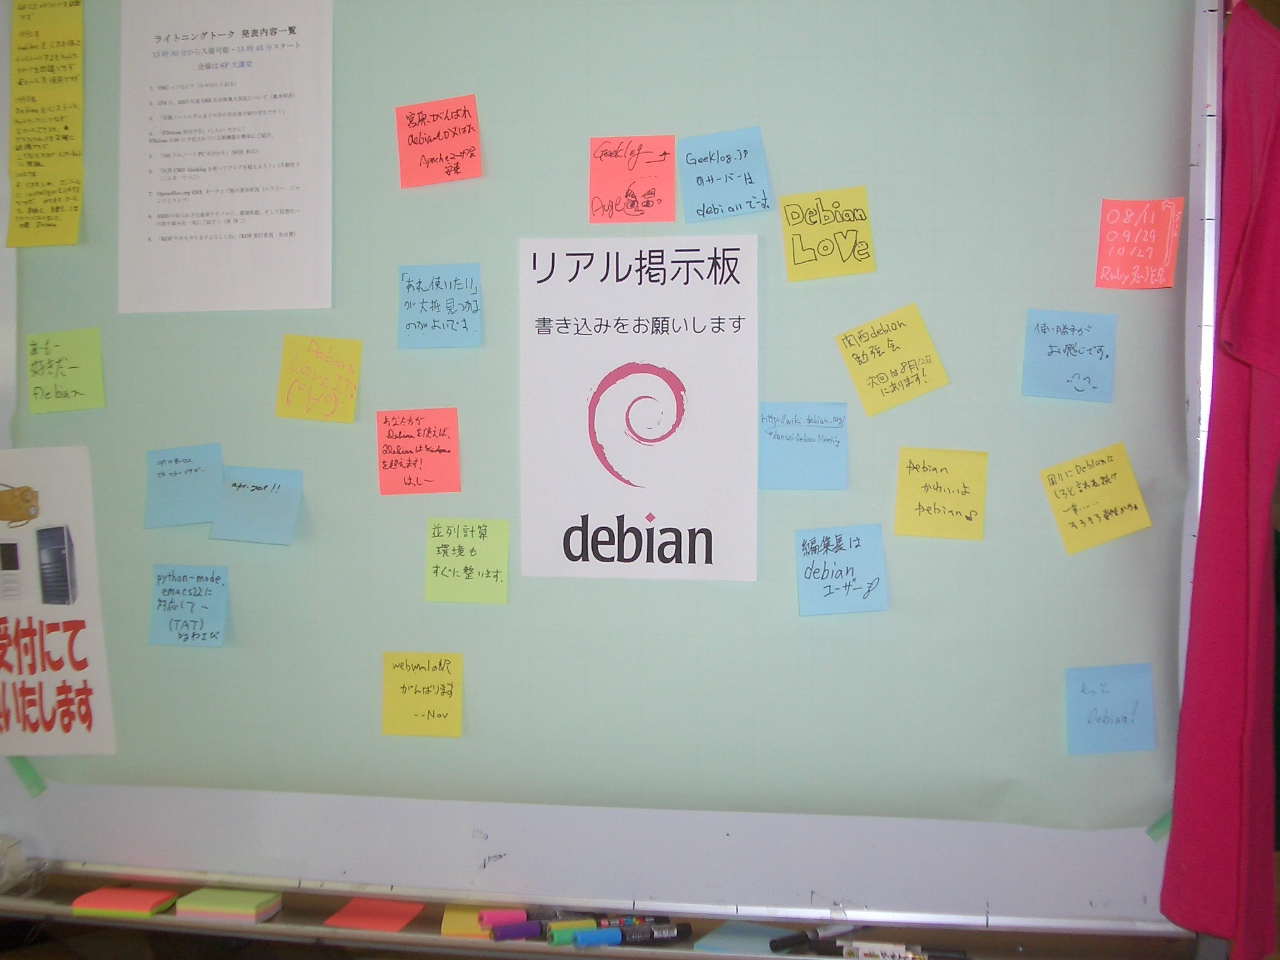
\includegraphics[width=\hsize]{image200708/real-keijiban.jpg}
\end{center}
\caption{$B%j%"%k7G<(HD(B}
\label{fig:realkeiji}
\end{figure}

$B=8$^$C$?0U8+$O2<5-$G$9!#(B

\begin{multicols}{2}
 \begin{itemize}
 \item Debian Love IT! \verb|$B!J!&"O!&!K(B|
 \item $B5\86$,$s$P$l(B debian $B$b$,$s$P$l(B Apache $B%f!<%62q(B $B0BEl(B
 \item $B!V$"$l;H$$$?$$!W$,BgDq8+$D$+$k$N$,$h$$$G$9(B
 \item Geeklog.JP $B$N%5!<%P$O(B debian $B$G!<$9!#(B
 \item Debian Love
 \item lilo.linux.or.jp $B$b(B Debian $B$GF0$$$F$$$^$9(B by ohura
 \item Sumibi.org $B$b(B Debian $B$GF0$$$F$$$^$9!*(B by kiyoka
 \item $BJT=8D9$O(B Debian $B%f!<%6!*(B
 \item $B$b$C$H(B Debian$B!*(B
 \item Debian $B$+$o$$$$$h(B Debian $B"v(B
 \item $B;H$$>!<j$,$h$$46$8$G$9!#(B
 \item $B<~$j$K(B Debian $B$K$7$m$H8@$o$lB3$10lG/!D$=$m$=$m3P8g$+$J$!(B
 \item apt$B$O;H$$$^$9$h!#$G$b%^%+!<$G$9$,!D(B
 \item apt-get !!
 \item python-mode emacs22 $B$KBP1~$7$F!<(B \verb|$B!J#T#A#T!K(B| by $B$o$5$S(B
 \item webwml$B$NLu$,$s$P$j$^$9(B --Nov
 \item $BJBNs7W;;4D6-$b$9$0$K@0$$$^$9!#(B
 \item $B$"$J$?J}$,(B Debian $B$r;H$($P!"(BDebian$B$O(BWindows$B$r1[$($^$9!*!!$O$C$7!<(B
 \item $B$"!<$b!<9%$-$@!<(B Debian
 \item 1998$BG/(B Debian $B$r%$%s%9%H!<%k!"%M%C%H%o!<%/$K7R$.!"(BE$B%a!<%k$G$-$k$b!"(B
       $B%0%i%U%#%C%/%+!<%I$r@53N$KG'<1$G$-$:!"(BLYNX$B$N$_$G%$%s%?!<%M%C%H$K(B
       $B@\B3!#(B
 \item 2007$BG/(B $B:#!"(BCD$B$rF~$l!"%3%s%=!<%k$K(B installguit $B$HF~NO$9$k$@$1$G!"(BWEB$B$b%a!<(B
       $B%k$b!"F02h$b!"2;3Z$b!"$7$[$&$@$$$K$J$j$^$7$?!#K|:P(B Debian
 \end{itemize}
\end{multicols}

$B%5!<%P$G$b%G%9%/%H%C%W$G$b!"K\Ev$K$_$J$5$s!"(BDebian $B$r0&$7$F$^$9$M(B
\verb|:)|

$B8D?ME*$K5$$K$J$C$?$N$O!"(Bpython-mode$B$K$D$$$F$G$9$,!"(BEmacs22$B$+$i(B
python-mode$B$OIUB0$9$k7A$KJQ99$5$l$?$_$?$$$G!";d$N(Bsid $B>e$N(BEmacs22$B$G$O(B
python-mode$B$,F0$$$F$$$^$9!#(B

\subsubsection{$BG[I[!&HNGdJ*(B}

$B0J2<$N$b$N$rG[I[$7$^$7$?!#(B

\begin{itemize}
 \item $B%U%i%$%d!<(B
 \item DVD
\end{itemize}

\begin{center}
 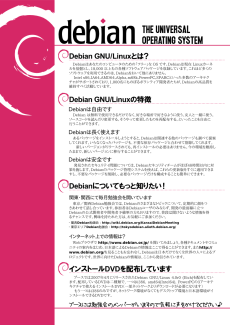
\includegraphics{image200708/flyer.png}
 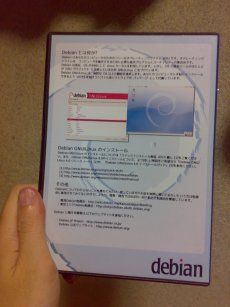
\includegraphics{image200708/dvd.jpg} 
\end{center}

$B4X@>(B Debian $BJY6/2q$G$O!"(BOSC Kansai $B$GG[I[$r9T$&$?$a$K!"Lp?a$5$s$,Ds0F$7(B
$B$FD:$$$?%U%i%$%d!<$r;29M$K!"F|K\?M8~$1$K:n$jBX$($k$?$a$K!"$N$,$?$5$s$,%G%6%$%s(B
$B$rC4Ev$7!"$+$,$5$s!"ARI_$5$s$J$I$,J8>O$r9M$($^$7$?!#(B

$B$^$?!"(BDVD$B%8%c%1%C%H$K$D$$$F$b!"$+$,$5$s$,%G%6%$%s$rC4Ev$7!"IpF#$5$s$N%$(B
$B%s%9%H!<%k%,%$%I$N(BURL$B$,=q$$$F$"$C$?$j!"%8%c%1%C%H$,3J9%$h$+$C$?$N$G!"2H(B
$B$K>~$j$^$9$H$*$C$7$c$i$l$?J}$b$$$i$7$c$$$^$7$?!#$?$@!"$h$jB?$/$NJ}$K(B
Debian $B$K$D$$$FCN$C$F$b$i$&$?$a$K!"(BDebian $B$r;H$C$F$$$i$C$7$c$kJ}(B
$B$K$O<~$j$N?M$KG[I[$7$F2<$5$$$H$*4j$$$7$^$7$?!#(B

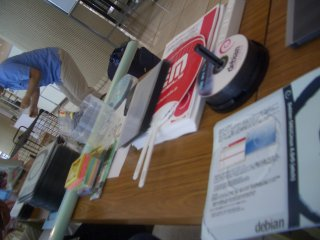
\includegraphics{image200708/booth2.jpg}
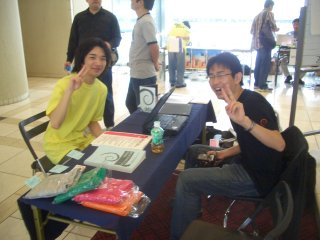
\includegraphics{image200708/booth.jpg}

$B0J2<$N$b$N$rHNGd$7$^$7$?!#(B

\begin{itemize}
 \item T$B%7%c%D(B
 \item $B%9%F%C%+!<(B
 \item $B!V$"$s$I$-$e$a$s$F$C$I(B $B$G$S$"$s!W(B2006$BG/E_9f$N:};R(B
\end{itemize}

$BNA6b$K$D$$$F$O!":#G/$N(B3$B7n$K9T$o$l$?(B OSC Spring $B$H0l=o$K$7!"(BT$B%7%c%D$H%7!<(B
$B%k$O>.<<$5$s!"!V$"$s$I$-$e$a$s$F$C$I(B $B$G$S$"$s!W$N:};R$O4d>>$5$s$K;d$N2H(B
$B$KAw$C$FD:$-!"0QBwHNGd$H8@$&7A$G9T$$$^$7$?!#(B
$BGX7J$H$7$F!";d$,4X@>(B Debian $BJY6/2q$K(B Debian T$B%7%c%D$rCe$F$$$/$H!"$d$O$j%0%C%:$,(B
$BM_$7$$$J$!$H8@$C$F$$$?$@$$$?$j!";fG^BN$G>pJs$,M_$7$$$C$FJ}$,$$$i$C$7$c$C(B
$B$?$N$G!"<B8=$7$^$7$?!#(B

$BEv=i!"KM$,M=A[$7$F$$$?$b$N$h$j$bB?$/$NGd$j>e$2$,$"$j!"$d$O$j:};R$G$_$?$$(B
$B$H8@$&0U8+$d!"(BT$B%7%c%D$N9u?'$,M_$7$$!"(BM$B%5%$%:$,M_$7$$$J$I$N0U8+$b$"$j$^$7(B
$B$?$N$G!"(B11$B7n(B9,10$BF|$KBg:eFn9A(BATC$B$G9T$o$l$k4X@>%*!<%W%s%=!<%9%U%)!<%i%`$G(B
$B$b%0%C%:$NHNGd$r9T$$$?$$$H;W$$$^$9!#(B

$BGd$j>e$2$G$9$,!"(BT$B%7%c%D!J(B1$BKg(B2000$B1_!K$,(B11$BKg!#:};R!J(B1$BIt(B1000$B1_!K$,(B7$BIt!#%9%F%C(B
$B%+!<!J(B1$BKg(B300$B1_!K$,(B12$BKg$G!"9g7W(B32,600
$B1_!J(B2000$B1_(B*11$BKg(B+1000$B1_(B*7$BIt(B+300$B1_(B*12$BKg!K$G$7$?!#$46(NOD:$$$?J}!"K\Ev$K$"$j$,$H$&$4$6$$$^$7$?!#(B

\dancersection{cdn.debian.or.jp$B$N>R2p(B}{$B9SLZ(B $BLw9((B (yasu@debian.or.jp, ar@debian.org)}
\label{sec:cdndebianorjp}
\index{debianjp@Debian JP}
\index{cdn.debian.or.jp}
\index{Content Delivery Network}

\subsection{CDN$B$H$O(B}

Content Delivery Network$B!J(BCDN$B!K$O%&%'%V%3%s%F%s%DG[CV$*$h$SG[AwJ}K!$H$7$F(B
Akamai\index{Akamai} $B<R$K$h$j%5!<%S%9$5$l9-$/CN$i$l$k$3$H$K$J$C$?!#Ev=i$+(B
$B$i0lIt$N?M5$$N9b$$%5!<%P$X$N%H%i%U%#%C%/=8Cf$K$h$k%5!<%PDd;_$N2sHr!"3$30(B
$B$N%j%C%A%3%s%F%s%D<hF@$N9bB.2=!"%H%i%U%#%C%/J,;6$K$h$k%M%C%H%o!<%/$*$h$S(B
$B%5!<%P$NMxMQJ?=`2=$J$I$NM}M3$G9-$/<u$1F~$l$i$l$?!#(B

CDN$B$H$$$&MQ8l<+BN$O(BWWW$B$K8B$k$3$H$J$/!"0lHL$K%3%s%F%s%D$r<hF@$9$k$?$a$NG[(B
$BAw<jCJ$dJ}K!A4BN$r;X$9>l9g$,$"$k!#$?$H$($P!"(BWinny\index{Winny} $B$d(B
Bittorrent\index{Bittorrent}$B$J$I$N%3%s%F%s%D$r<hF@$9$k$?$a$KFCJL$K@_7W$5(B
$B$l$?%W%m%H%3%k$rMQ$$$F!"(BP2P$B%M%C%H%o!<%/$r9=@.$9$k$h$&$J<jK!$b4^$^$l$k!#(B

\subsection{Debian$B$K$*$1$k(BCDN$B$N8=>u(B}
\subsubsection{$BMxMQK!$H%f!<%6$+$i8+$?F0:n(B}

\url{cdn.debian.or.jp}$B$G$O(BDebian$B$G%$%s%9%H!<%k;~$+$i9-$/(Bdeb$B%U%!%$%k$NF~<j$K;H(B
$B$o$l$k(Bapt$B$G;H$($k(BCDN$B$H$7$F@_7W$7!"1?MQ$7$F$$$k!#$=$N$?$a!"(BDebian$B$K$*$1$k(B
CDN$B$NMxMQK!$O;j6K4JC1$G$"$k!#(B\url{/etc/apt/source.list} $B$K5-=R$9$k(BAPT $B%j%]%8%H(B
$B%j$H$7$F!"(B

\begin{commandline}
 deb http://cdn.debian.or.jp/debian/ stable main contrib non-free
 deb-src http://cdn.debian.or.jp/debian/ stable main contrib non-free
\end{commandline}

$B0J>e$N$h$&$K;XDj$9$k$@$1$G%f!<%6$O:#$^$G$H$J$s$iJQ$o$k$3$H$J$/(Bapt$B%3%^%s%I(B
$B$r;HMQ$G$-$k!#%5!<%S%9;~$N<j=g$H9=@.$O0J2<$N$h$&$K$J$k!#(B
$B!J(B\fgref{fig:usercdndebianorjp}$B!K(B

\begin{enumerate}
 \item  $B%f!<%6$,(Bapt-get $B%3%^%s%I$r9T$&$H(Bcdn.debian.or.jp$B$r(BDNS$B$GLd$$9g$o$;$k(B
 \item  \url{cdn.debian.or.jp}$B$r4IM}$9$k(BDNS$B$O%5!<%P8uJd(B(surrogate)$BA*Br$9$k(B
 \item  $BA*Br7k2L$r(BDNS$B$N%j%W%i%$$H$7$FJV$9(B
 \item  apt$B$O(B\url{cdn.debian.or.jp}$B$H$7$F(BSurrogate C$B$r;HMQ$9$k(B
\end{enumerate}

\begin{figure}[H]
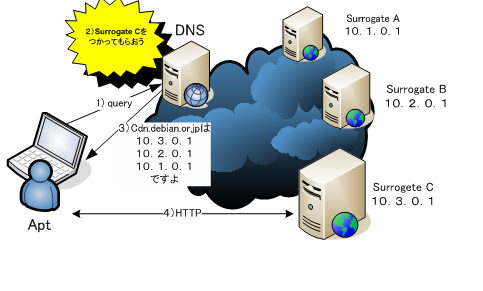
\includegraphics[width=\hsize]{image200708/surrogate.png}

 \caption{$B%f!<%6$+$i8+$?(Bcdn.debian.or.jp$B$NF0:n(B}
 \label{fig:usercdndebianorjp}
\end{figure}

\subsubsection{cdn.debian.or.jp$B$N%7%9%F%`$HF0:n(B}
CDN$B%7%9%F%`$,40A4$KF0:n$7%f!<%6$+$i;HMQ$5$l$k$?$a$K$O!"%7%9%F%`$,40A4$J(B
$B%U%!%$%k$rDs6!$9$k$3$H!"%7%9%F%`$,0BDj$7$FF0:n$9$k$3$H!"$=$7$F(BCDN$B$r;H$C(B
$B$?>l9g$K9bB.$KF0:n$7$F$$$k$3$H$,5a$a$i$l$k!#(B

\subsubsubsection{$BDs6!%U%!%$%k$N40A4@-(B}

$B$3$N$?$a$K0J2<FsE@$rK~$?$5$M$P$J$i$J$$!#(B
\begin{itemize}
 \item  $B8D!9$N%U%!%$%k$,%3%s%F%s%DDs6!<T$?$k(Bdeb$B%U%!%$%kG[I[85$HF10l$G$"$k$3$H(B
 \item  apt-get update$B$N7k2L<hF@$9$k%U%!%$%k72$,$I$N(BSurrogate$B$G$bF~<j$G$-$k$3$H(B
\end{itemize}
$BA0<T$K$D$$$F$O!"(Bdeb$B$O$=$N%U%!%$%k$N(Bmd5$BCM!"(Bsha1$BCM$H$H$b$KG[I[$5$l!"%f!<%6(B
$B$,;HMQ$9$k(Bapt$B$G3NG'8e$KMxMQ$5$l$k$?$a(BCDN$B$r;HMQ$7$?>l9g$G$bLdBj$K$J$i$J$$!#(B

$B8e<T$K$D$$$F$O%f!<%6$,(Bapt-get update$B$r9T$C$?$H$-$K@\B3$9$k(BSurrogate$B$H(B
apt-get dist-upgrade$B$r9T$C$?$H$-$K@\B3$9$k(BSurrogate$B$OF10l$G$"$k$H$O8B$i$J(B
$B$$$?$a!"(BDNS$B$,(BSurrogate$B$H$7$FJV$9%5!<%P$,J];}$9$k%U%!%$%k$OF10l$G$"$kI,MW(B
$B$,$"$k!#(B\url{cdn.debian.or.jp}$B$G$O(BDebian$B%W%m%8%'%/%H$G0lHL$K9T$o$l$F$$$k(B
$BJ}K!$HF1MM$K!"(Brsync$B%W%m%H%3%k$rMQ$$!"(Bpush$B%_%i!<$r9T$C$F$$$k!J?^#2!K!#$=$N(B
$B$?$a!"(B\url{cdn.debian.or.jp}$B$N%5%m%2!<%HFb$G:G>eN.$K$"$k%5!<%P$H%_%i!<$,(B
$BF10l$G$"$k$3$H$r(B2$BJ,Kh$K(Brsync$B%_%i!<=*N;;~$K:n@.$5$l$k%9%?%s%W%U%!%$%k$r3N(B
$BG'$7$F!"F10l$G$J$$%5!<%P$O%5%m%2!<%H8uJd$+$i0l;~E*$K=|30$7$F$$$k!#(B

\begin{figure}[H]
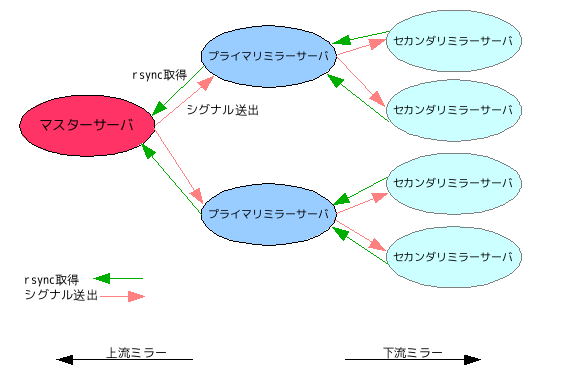
\includegraphics[width=\hsize]{image200708/pushmirror.png}
 \caption{Debian$B%5%m%2!<%H$N(Brsync$B$K$h$k%_%i!<(B}
 \label{fig:rsyncsurrogatemirror}
\end{figure}

\subsubsubsection{$B%7%9%F%`$N0BDjF0:n(B}
$B@h$K=R$Y$?$h$&$K!"%f!<%6$O(BCDN$B$r;HMQ$9$k:]$K$O(BDNS$B$r:G=i$K;HMQ$9$k$?$a!"(B
DNS$B$N0BDj1?MQ$,%+%.$H$J$k!#$=$N$?$a!"(B\url{cdn.debian.or.jp}$B$r4IM}$9$k(BDNS$B%5!<%P(B
$B$O$^$C$?$/FHN)$KF0:n$9$k%5!<%P$G9T$C$F$$$k!#(B

$B$^$?!"%5!<%P$NF0:n$r3NG'$O!"(B5$BIC0JFb$K(BHTTP$B$N%l%9%]%s%9$rJV$5$J$$%5!<%P$O(B
$B%5%m%2!<%H8uJd$+$i0l;~E*$K=|30$7$F$$$k!#(B

\subsubsubsection{$B9bB.F0:n(B}
\url{cdn.debian.or.jp}$B$G$O(BDNS$B$GLd$$9g$o$;$5$l$k$H%5%m%2!<%H%j%9%H$H$7$FJ#?t$N(B
IP$B%"%I%l%9$rJV$9!#$3$N(BIP$B%"%I%l%9$O%i%&%s%I%m%S%s$GA*Br$7$F$$$k$o$1$G$O$J(B
$B$/!"%5!<%P%-%c%Q%7%F%#$d%M%C%H%o!<%/B.EY$r9MN8$7!"@_Dj$7$F$$$k!#(B

\subsection{$B>-Mh$NE8K>(B}

$B$3$3$^$G@bL@$7$F$-$?!"(B\url{cdn.debian.or.jp}$B$NF0:n$K$O2~A1$9$Y$-E@$,B??tB8:_$9(B
$B$k!#2~A1$NE8K>$H$7$F$$$/$D$+5s$2$k!#(B

\subsection{apt-get$B%3%^%s%I$N(BHTTP REDIRECT}
apt-get$B%3%^%s%I$O(BHTTP REDIRECT$B$KBP1~$7$F$$$J$$!#(B

HTTP REDIRECT$B$O!"$$$C$?$s(BHTTP GET$B$J$I$G@\B3$7$F$-$?%/%i%$%"%s%H$KBP$7$F!"(B
$B?7$?$K$=$N%j%=!<%9$,B8:_$9$k(BURL$B$rDLCN$9$k$b$N$G$"$k!#$3$N;EAH$_$r$&$^$/(B
$B$D$+$C$?(BCDN$B$H$7$F!"(BCoral Content Distribution Network (Coral CDN)$B$,$"$k!#(B
Coral CDN$B$O%5%m%2!<%H4V$G(BP2P$B$K$h$k%U%!%$%kG[CV$7!"$=$N%$%s%?!<%U%'!<%9$H(B
$B$7$F!"(BHTTP$B$r;HMQ$7!"$7$+$b;HMQ$K$O%$%s%?!<%M%C%H$+$i<hF@2DG=$J%U%!%$%k$G(B
$B$"$l$P@)8B$r$+$1$F$$$J$$!#$5$i$K!"(BApache$B$r;H$C$?0l;~G[I[%5!<%P$G$O(BHTTP
REDIRECT$B$r$D$+$C$F(BCoral$B!!(BCDN$B$KM6F3$9$k$3$H$b?d>)$5$l$F$$$k!#$?$@$7!"8=>u(B
$B$G!"(BCoral CDN$B$r;H$&$?$a$K!"(B

\begin{commandline}
 deb http://cdn.debian.or.jp.nyud.net:8090/debian/ stable main contrib non-free
\end{commandline}
$B$r;XDj$9$k$3$H$b2DG=$@$,!">/$J$/$H$bF|K\$K$*$$$F$O(BCoral CDN$B$rC4$&%5%m%2!<(B
$B%H$,B8:_$7$J$$$3$H$b$"$C$FHs>o$KDcB.$G$"$k!#$?$@$74Z9q$dCf9q$G$O9-$/$D$+(B
$B$o$l$F$*$j!">-Mh$N3HD%$K;HMQ$7$?$$!#(B

\subsubsection{IP$B%"%I%l%9$N0LCV>pJs$r;HMQ$7$?%5!<%PA*Br(B}

global$B$K(BCDN$B$rE83+$9$k>l9g$K$OCOM}E*$K6a$$%5!<%P72$+$i$"$kDxEY9J9~$`$N$,(B
$BM-8z$G$"$k!#8=:_!"(BGeoIP$B$J$IL5NA$G(BIP$B$HCOM}>pJs$N%^%C%T%s%0Ds6!<T$,8=$l$F(B
$B$*$j!"$3$N3hMQ$O(B\url{cdn.debian.or.jp}$B$N<!$N3HD%$H$7$F:GM-NO$@$H9M$($F$$$k!#(B

\subsubsection{apt$B$N(BP2P$BBP1~(B}

$B8=:_!"(B\url{http://wiki.debian.org/DebTorrent} $B$d(B
\url{http://www.cs.sfu.ca/~camerond/personal/GoogleSoCDebian.html}$B$G(Bapt$B$N(B
Bittorrent$BBP1~$,?J$a$i$l$F$*$j!"M-NO$J8uJd$G$"$k!#$?$@$7!"(BBittorrent$B%W%m(B
$B%H%3%k$r%/%i%$%"%s%H$GD>@\;H$&$b$N$G$"$j!"%M%C%H%o!<%/MxMQ%]%j%7!<$H$N6%(B
$B9g$d(Binstall$B;~$KMxMQ2DG=$J$N$+$J$I:#8e8!>Z$9$Y$-LdBj$bB?$$!#(B


\subsection{$B$*$o$j$K(B}

$B$$$D$G$bI,MW$J%=%U%H%&%'%"$d%3%s%F%s%D$r0B2A$KF~<j$9$k<jCJ$H$7$F(BCDN$B$O$3(B
$B$l$+$i$bMM!9$JH/E8$rB3$1$k$H9M$($k!#(BDebian$B$O(Bdeb$B$N0BDjF~<j<jCJ$NM-L5$,%7(B
$B%9%F%`$N?.Mj@-$r:81&$9$k%7%9%F%`$G$"$j!"(BCDN$B$N9-HO$J3hMQ$,:#8e$^$9$^$95a(B
$B$a$i$l$k$h$&$K$J$k$H9M$($k!#(B


\dancersection{Debian GNU/kFreeBSD $B$N%$%s%9%H!<%k(B}{$B>e@n(B $B=c0l(B}
\label{sec:debiankfreebsd}
\index{FreeBSD}
\index{Debian GNU/kFreeBSD}

\subsection{$B$O$8$a$K(B}

$B:G6a$a$C$-$jOCBj$N(B Debian GNU/kFreeBSD $B$r(B qemu $B$G%$%s%9%H!<%k$7$F$_$^$7$?!#(B

\subsection{CD$B%$%a!<%8$N<hF@(B}

Debian GNU/kFreeBSD$B$N%Z!<%8(B
\url{http://www.debian.org/ports/kfreebsd-gnu/}$B$+$i%j%s%/$r$?$I$j!":#2s$O(B
\url{http://glibc-bsd.alioth.debian.org/install-cd/kfreebsd-i386/20070313/}
$B$+$i(B debian-20070313-kfreebsd-i386-install.iso $B$r<hF@$7$^$7$?!#(B

\url{http://glibc-bsd.alioth.debian.org/doc/} $B$KJ8=q$,$"$j$^$9!#(B

\subsection{qemu $B$N=`Hw(B}

$B$^$:!"%G%#%9%/%$%a!<%8$r:n@.$7$^$9!#(B

\begin{commandline}
qemu-img create -f qcow f.cow 4G
\end{commandline}

\subsection{$B%$%s%9%H!<%i$N5/F0(B}

qemu $B$G(B ISO $B%$%a!<%8$+$i5/F0$7$^$9!#6qBNE*$J%3%^%s%I%i%$%s$O$3$N$h$&$K$J(B
$B$j$^$9!#!JI.<T$N%7%9%F%`$O(B amd64 $B%"!<%-%F%/%A%c$N$?$a!"(B kqemu $B$r3hMQ$9$k(B
$B$?$a$K!"(Bqemu-system-x86\_64 $B$rMxMQ$7$F$$$^$9!#(Bi386$B$G$"$l$P!"(B qemu $B%3%^%s%I(B
$B$r$+$o$j$KMxMQ$7$^$9!#(B)

\begin{commandline}
qemu-system-x86_64 -hda f.cow \
 -cdrom debian-20070313-kfreebsd-i386-install.iso \
 -m 256 -boot d 
\end{commandline}



Express$B$rA*Br!"E,Ev$K%Q!<%F%#%7%g%s$r@Z$C$F$_$F!"(BFreeBSD$B$N%V!<%H%m!<%@$r(B
$BMxMQ$7$F$_$^$7$?!#%^%K%e%"%k$K$7$?$,$C$FE,Ev$KEz$($F$$$-$^$9!#(B
$B%$%s%9%H!<%kBP>]$O(B Minimal $B$rA*Br$7$F!"%$%s%9%H!<%k$rB39T$7$^$9!#(B

\begin{figure}[H]
 \begin{multicols}{2}
 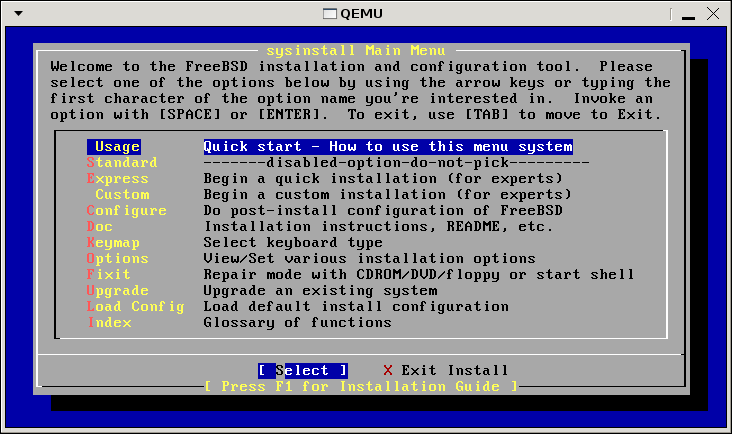
\includegraphics[width=\hsize]{image200708/kfreebsd-install-0.png}
 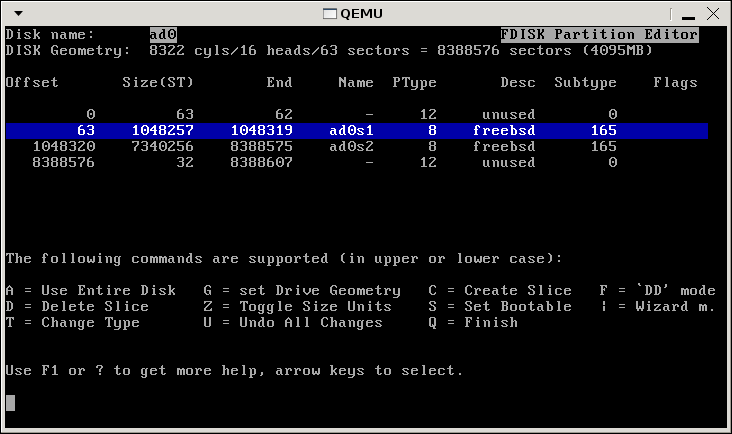
\includegraphics[width=\hsize]{image200708/kfreebsd-install-1.png}
 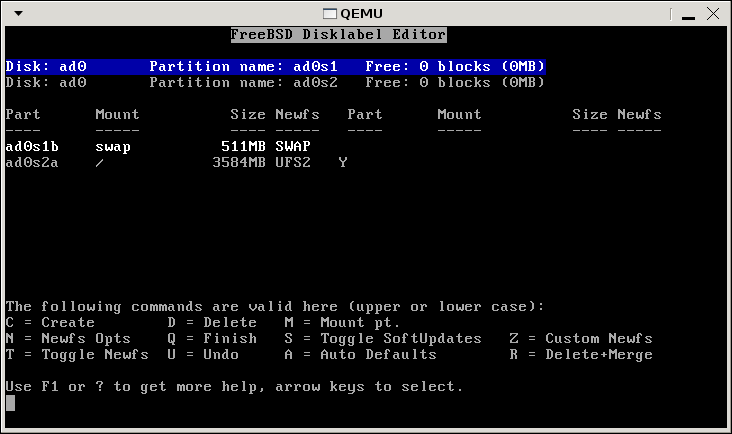
\includegraphics[width=\hsize]{image200708/kfreebsd-install-2.png}
 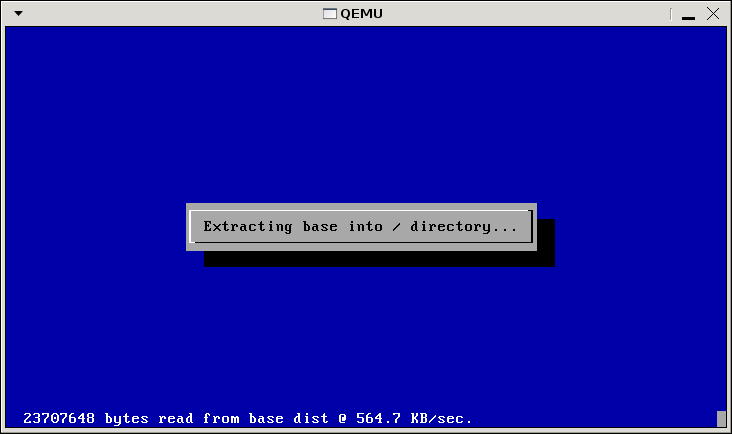
\includegraphics[width=\hsize]{image200708/kfreebsd-install-3.png}
 \end{multicols}
\caption{Debian GNU/kFreeBSD $B%$%s%9%H!<%k2hLL(B}
\label{fig:kfreebsdinst}
\end{figure}

$B$7$P$i$/BT$D$H(B alt-f3 $B$G2hLL$r@Z$jBX$($m$HI=<($5$l$^$9!#(B
debconf $B$N<ALd$KEz$D$D%$%s%9%H!<%k$,$D$E$-$^$9!#(B

\begin{figure}[H]
 \begin{center}
  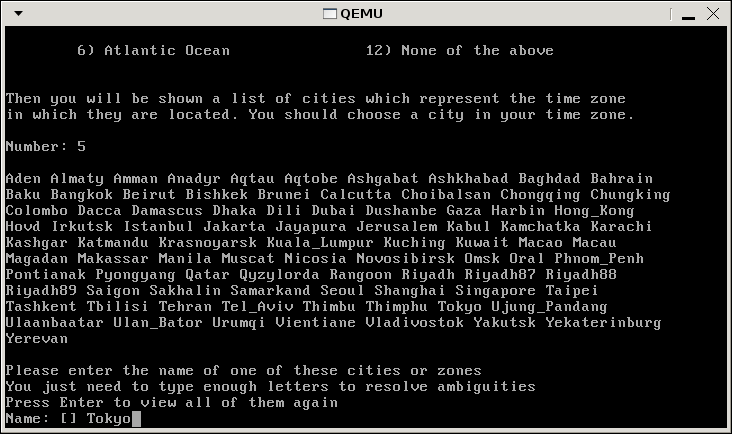
\includegraphics[width=0.5\hsize]{image200708/kfreebsd-install-4.png}
 \end{center}
 \caption{$B=i4|%Q%C%1!<%8%$%s%9%H!<%k!&@_DjCf(B}
 \label{fig:kfreebsdinst2}
\end{figure}

$B:G8e$K%j%V!<%H$r$9$k$h$&$K;X<($5$l$k$N$G!"$=$3$G(B
qemu $B$r0lC6=*N;$7$^$9!#(B

$B$3$3$G!"(B qemu $B$r(B HDD $B%$%a!<%8$+$i5/F0$9$k$h$&$K$7$F<B9T$7$^$9!#(B

\begin{commandline}
 qemu-system-x86_64 -hda f.cow -m 256 
\end{commandline}

$B5/F0$9$k$H!"$J$<$@$+(B root filesystem $B$,(B read-only $B$@$+$i$H$$$m$$$m$H<:GT(B
$B$7$^$9!#(B
fsck $B$,I,MW$J>l9g$N5/F0$KITET9g$,$"$k$h$&$G$9!#(B
$B0lC6(B root $B$G%m%0%$%s$7!"(Breboot $B%3%^%s%I$G%j%V!<%H$7$F$_$k$H(B root
filesystem $B$r@5>o$K%^%&%s%H$9$k$3$H$,=PMh$k$h$&$G$9!#(B

$B$^$?!"(B /etc/network/interfaces $B$,$^$C$?$/@_Dj$5$l$F$$$J$$>uBV$J$N$G!"%M%C%H%o!<(B
$B%/$,;H$($J$$>uBV$G5/F0$7$F$-$^$9$,(B dhclient $B$r<B9T$9$l$P(BIP$B$r<hF@$7$F2TF/(B
$B$9$k$3$H$b2DG=$G$9!#(B

\begin{commandline}
 dhclient ed0
\end{commandline}

\subsection{$BF0$$$?!*(B}

$B$3$l$GL5;v$K(B Debian GNU/kFreeBSD $B$N2TF/$,3NG'$G$-$^$7$?!#(B
$B$^$@$^$@40@.EY$,;j$i$J$$E@$,B?$$$N$G!"%G%P%C%0$7$[$&$@$$$G$9!#(B

 \begin{figure}[H]
  \begin{center}
   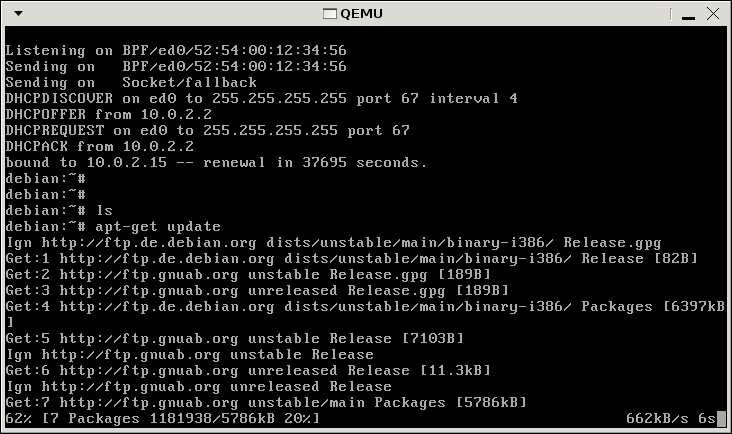
\includegraphics[width=0.5\hsize]{image200708/kfreebsd-install-5.png}
  \end{center}
  \caption{Debian GNU/kFreeBSD $B$G(B apt-get $B$7$F$_$^$7$?(B}
  \label{fig:kfreebsdaptget}
 \end{figure}
 
\dancersection{Exim $B:FH/8+(B}{$B>.<<(B $BJ8(B}
\label{debianexim}
\index{exim}
\subsection{intro}
$B;dC#$NF|>o$G$O%a!<%k$O7g$+$;$J$$%3%_%e%K%1!<%7%g%s%D!<%k$G$9!#(B
$B$=$l$r<B8=$9$k0Y$K!"F3F~$5$l$k(B MTA( Mail Transfer Agent )$B$O!"$I$N%=%U%H$r;H$C$?$i(B
$B0lHV%3%9%H%Q%U%)!<%^%s%9$,NI$$$+!"$^$?$I$&$d$C$?$i2q<R!"%0%k!<%W!"8D?M$N%K!<%:$KEz$($k;v$,(B
$B=PMh$k$+!"%7%9%F%`4IM}<T$OF|LkF,$rG:$^$7$F$$$k$O$:$G$9!#$=$7$F0lEYF3F~$7$?%a!<%k%5!<%P!<$N(B
$B;EAH$_$O!"$J$+$J$+JL$N;EAH$_$K>h$j49$($k$N$O!";~4V$HHqMQ$,$+$+$j!"LdBj$,$"$C$?$H$7$F$b$J$+(B
$B$J$+0\9T$7$E$i$$$H$$$&8=>u$b$"$j!"(BMTA$B$r7h$a$k$N$O?M@8$G$J$+$J$+K,$l$J$$Bg7h?4$N0l$D$G$"$k(B
$B;v$OL@Gr$G$9!#(B
MTA $B$N0l$D!"(BExim $B$O(B Debian $B$N(B Default MTA $B$H8F$P$l$J$,$i$b!":#$d(B Postfix $B$N?M5$$K(B
$B$9$C$+$j1F$r@x$a$F2a5n$N1I8w$K4E$s$8$F$$$k$N$,8=<B$G$9!#(B
$B:#F|$O(B Exim $B$NNr;K!"MxE@!&ITMxE@!"F3F~J}K!$r8f>R2p$7$^$9!#(B $B3'$5$s$N(B MTA $B$KA*$P$l$J$+$C$?(B
$B$H$7$F$b!"(BExim $B$O$3$&$$$&%Q%C%1!<%8$J$N$+!*$HCN$C$FD:$1$l$P9,$$$G$9!#(B

\subsection{Exim$B$H$O(B}
Exim\footnote{Exim $B$NL>A0$NM3Mh$O(B EXperimental Internet Mailer (Exim)}
 $B$H$O!"(BUnix$B$b$7$/$O(B Unix like $B$J(BOS$B$N>e$GF0$/(B Mail Transfer Agent $B$G$9!#(BCygwin 
$B$r;H$($P(B Windows $B$N>e$G$bF0$+$9;v$,=PMh$^$9!#(BExim $B$O%1%s%V%j%C%8Bg3X$G(B 1995 $BG/$K(B Philip Hazel 
$B$5$s$K$h$C$F3+H/$5$l$^$7$?!#(B\\

\subsection{Exim $B$NNr;K(B}
$B%1%s%V%j%C%8Bg3X$G$O!"J#?t$N(B MTA $B$,F0$$$F$$$F(B(Sendmail, Smail, PP$B!)$J$I$J$I(B)$B!"$=$s$J4D6-(B
$B$K$&$s$6$j$7$F$?$,$I$&$+$OITL@$G$9$,!"(BPhilip Hazel $B$5$s$O(B Smail $B$r3HD%$7$F(B MTA $B$rBg3X$N%K!<%:(B
$B$K9g$o$;$F:n$m$&$H;n$_$^$7$?!#$7$+$7;DG0$J$,$i!"(BSmail $B3HD%$O$"$C$5$jD|$a!"(BHazel $B$5$s$O%9%/%i%C%A(B
$B$+$i(B MTA $B$r:n$m$&$H;n$_$k;v$K$7$^$7$?!#(B
$B$=$N:n6H$,!"H`$,=jB0$7$?(B Computer Sceince $B$NCg4V$KCN$l$o$?$j!"(BFTP $B%5!<%P!<$rN)$F$i$l!"G[I[$5$l(B
$B$k$h$&$K$J$j$^$7$?!#(B
$B=q$$$F$$$kESCf$GG[I[$,$5$l$k$h$&$K$J$C$?0Y!"@5<0$J(B Exim 0 $B$b$7$/$O(B 1 $B$O%j%j!<%9$7$F$$$^$;$s(B
($B>/$J$/$H$b(B Hazel $B$5$s$O%j%j!<%9=PMh$J$+$C$?$H;W$C$F$$$k$h$&$G$9(B)$B!#(B\\
$B85!9(B Sendmail, Smail $B$r?($C$F$$$?(B Hazel $B$5$s$O(B Sendmail $B$KBe$o$k(B MTA $B$r:n$m$&$H(B Exim 
$B$r@_7W$5$l$F$$$^$9!#(B \\
\begin{tabular}[htb]{|l|l|} \hline
1995$BG/!)7n(B & Exim $B3+H/3+;O(B\\ \hline
1995$BG/(B11$B7n(B & $BF1N=$,(B FTP $B%5!<%P$r$D$/$j%Q%C%1!<%8$rG[I[;O$a$k!#%/%A%3%_$G9-$,$k(B\\ \hline
1998$BG/2F(B & Perl $B$N@55,I=8=%i%$%V%i%j!<$,$J$+$C$?$N$G:n$k(B(PCRE)\\ \hline
1999$BG/(B3$B7n(B & $B%3!<%I%M!<%`(B Slink $B$N(B Debian 2.1 $B%j%j!<%9!#(B Exim $B$r%G%#%U%)%k%H(B MTA $B$H$7$F5/MQ$9$k(B \\ \hline
1999$BG/(B9$B7n(B & $B%1%s%V%j%C%8Bg3X$G(B Exim $B$N9V:B$r3+;O$9$k!#(B \\ \hline
2000$BG/(B8$B7n(B & $B%3!<%I%M!<%`(B potato $B$N(B Debian 2.2 $B%j%j!<%9(B\\ \hline
2002$BG/(B7$B7n(B & $B%3!<%I%M!<%`(B woody $B$N(B Debian 3.0 $B%j%j!<%9(B\\ \hline
2004$BG/(B5$B7n(B & $B%1%s%V%j%C%8Bg3X$,(B Exim $B$r@5<0$K%5%]!<%H$9$k$H@k8@(B\\ \hline
2005$BG/(B6$B7n(B & $B%3!<%I%M!<%`(B sarge $B$N(B Debian 3.1 $B%j%j!<%9(B\\ \hline
2007$BG/(B4$B7n(B & $B%3!<%I%M!<%`(B etch $B$N(BDebian 4.0 $B%j%j!<%9(B\\ \hline
\end{tabular}

\subsection{Exim $B$H(B Debian $B$N4X78(B}
\subsubsection{$B8=:_$N(B Exim $B$N%a%s%F%J!<(B}
$B8=:_$N(B Exim $B$N%a%s%F%J!<$O(B
\begin{itemize}
\item Andreas Metzler  \url{ametzler@debian.org}
\item Marc Haber \url{mh@debian.org}
\end{itemize}
$B$G$9!#(B
Slink $B$G(B Exim $B$,Ek:\$5$l$k$h$&$K$J$kA0$+$i!"(BSendmail $B$d(B Smail $B$+$i(B Exim $B$X0\9T$r;n$_$k?M$,Bt;3$$$?(B
$B$h$&$G$9!#(B
$BF|K\$G$O%^%K%e%"%k$NF|K\8l2D$,$"$^$j?J$^$:(B($B8=:_$b>.?t$N?MC#$,:n6H$7$F$$$k$N$_(B)$B!"(BSlink $B$G(B Exim $B$,Ek:\$5$l(B
$B$?$N$G!"0\9T$7$?!"$H$$$&?M$,B?$+$C$?$h$&$G$9!#(B

\subsubsection{$B$J$<(B Exim $B$O(B Debian $B$N(B Default MTA $B$K$J$C$?$N$+!*!)(B}

\begin{tabular}[htb]{|l|l|} \hline
1996$BG/(B09$B7n(B & Tim Cutt $B$,(B Debian $B$G(B Exim $B$r%Q%C%1!<%8$H$7$FDs6!$9$k0Y$K:n6H$r;O$a$k(B \\ \hline
1997$BG/(B05$B7n(B & Exim $B$,(Bunstable $B$KF~$k(B by David Sewell \\ \hline
1999$BG/(B03$B7n(B & Slink $B$G(B Exim $B$r%G%#%U%)%k%H(B MTA $B$H$7$F5/MQ$9$k!#(B\\ \hline
\end{tabular}

$BEv;~$O(B Postfix$B!"(BSendmail, Smail $B$J$I$,$"$C$?$j$^$7$?$,!"%i%$%;%s%9LdBj(B
\footnote{$B%i%$%;%s%97ABV!'(BGNU General Public License (GPL)  ver2}
$B!"5!G=$N=<<BEY9g$J$I$,$"$j!"(B
Debian $B$N(B Defualt MTA $B$K$J$C$?$h$&$G$9!#(B

\subsection{Exim $B$HB>$N(B MTA $B$NAj0cE@(B}

\begin{tabular}[htb]{|l|ccc|} \hline
MTA&$B%i%$%;%s%97ABV(B & $B%a%$%s@=:n<T(B & $B%j%j!<%9>uBV(B \\ \hline
qmail&DJB$B%i%$%;%s%9(B&D. J. Bernstein& 1997$BG/$K=P$7$?$C$-$j(B\\ \hline
Postfix&IBM Public License&Wietse Zweitze Venema&1997$BG/$K%j%j!<%98e!"ETEYETEY$K%j%j!<%9(B \\ \hline
Exim&GPL&Philip Hazel&1995$BG/$K%j%j!<%98e!"ETEYETEY%j%j!<%9(B \\ \hline
\end{tabular}

{\Large qmail}
\begin{itemize}
\item 1997$BG/$+$i%j%j!<%9$5$l$F$$$J$$!#(BIPv6 $B$KBP1~$7$F$J$$!#%i%$%;%s%97ABV!"F3F~$,Fq$7$$(B
\item $BBgNL%a!<%k$rG[?.$9$k>l9g!"%;%-%e%j%F%#!<LL(B
\end{itemize}

{\Large Postfix}
\begin{itemize}
\item Exim $B$[$I5!G=$N<BAu$,$J$$(B
\item $B0\9T$,4JC1!"%3%_%e%K%F%#!<$,%"%/%F%#%V!"F|K\$G$b;H$C$F$$$k%f!<%6!<$,B?$$(B($BK\$bB?$$(B)
\end{itemize}

{\Large Exim}
\begin{itemize}
\item $BF|K\8l$N%^%K%e%"%k$,$J$$(B
\item $B%3%_%e%K%F%#!<$,%"%/%F%#%V!"(BDebian $B$N(B Default MTA$B!"%i%$%;%s%9!"%I%-%e%a%s%H$,K-IY(B($B1Q8l(B)
\end{itemize}

\subsection{Exim $B$N@_DjJ}K!(B}
\subsubsection{$B4{B8%Q%C%1!<%80lMw(B}
$B8=:_$N(B Debian $B$N(B stable $B$G$"$k(B etch $B$K$O0J2<$N(B Exim $B8~$1%Q%C%1!<%8$,MQ0U$5$l$F$$$^$9!#(B

\begin{tabular}[htb]{|l|l|} \hline
exim4&Exim 4 $B$r4JC1$K%$%s%9%H!<%k$9$k0Y$K%a%?%Q%C%1!<%8(B\\ \hline
exim4-base&$BA4(B Exim 4 $B%Q%C%1!<%8;Y1g%Q%C%1!<%8(B\\ \hline
exim4-config&Exim 4 $B@_DjMQ%Q%C%1!<%8(B \\ \hline
exim4-daemon-heavy&$BDI2C5!G=(B(exiscan-acl$B4^$`(B)$B$rEk:\$7$F$$$k%G!<%b%s%Q%C%1!<%8(B\\ \hline
exim4-daemon-light&$B4J0W5!G=$rEk:\$7$F$$$k%G!<%b%s%Q%C%1!<%8(B\\ \hline
exim4-daemon-light-dbg&debug$BMQ(B\\ \hline
exim4-dbg&debug$BMQ(B\\ \hline
exim4-dev&$B%X%C%@!<%U%!%$%kMQ$N(B Exim 4 $B%Q%C%1!<%8(B \\ \hline
exim4-doc-html&Exim 4 $B$N(B html $B7A<0$N%I%-%e%a%s%H%Q%C%1!<%8(B\\ \hline
exim4-doc-info& Exim 4 $B$N(B info $B7A<0$N%I%-%e%a%s%H%Q%C%1!<%8(B\\ \hline
\end{tabular}

\subsubsection{$B%$%s%9%H!<%kJ}K!(B}

\begin{commandline}
aptitude install exim4 exim4-base exim4-config exim4-daemon-heavy
\end{commandline}
$B$+(B
\begin{commandline}
aptitude install exim4 exim4-base exim4-config exim4-daemon-light
\end{commandline}
$B$r<B9T$7$^$9!#(B

exim-config $B$K$h$C$FI,MW$J>pJsF~NO$O%W%m%s%W%H$,=P$k$N$G;X<($K=>$$$^$9!#(B \\
\begin{enumerate}
\item $B@_Dj%U%!%$%k$rJ,3d$9$k$+!"H]$+(B
\item $B%a!<%k$N07$$$K$D$$$F(B($BAw?.%5!<%P$N7hDj(B)
\item $B%a!<%k%I%a%$%sL>$K$D$$$F(B
\item $B<u$1$D$1$k%a!<%kAw?.85$N(B IP $B@)8B$N7hDj(B( IPv6 $BBP1~(B)
\item Virtual Domain $B$N2<=`Hw(B
\item $B%*!<%W%s%a!<%k$N@_Dj(B
\item $B%m!<%+%k%M%C%H%o!<%/$+$i$NAw?.$N7hDj(B
\item $B%@%$%d%k%"%C%W;~$N(BDNS look up$B$N7hDj(B
\item $B%a!<%k7A<0$N7hDj(B(mbox/Maildir)
\end{enumerate}

\subsection{Exim $B$N$3$l$+$i(B}
 Philip Hazel $B$5$s$O(B2007$BG/(B2$B7n(B8$BF|IU$G!"(B9$B7nKv$K(B Exim $B$+$i0zB`$7$?$$$H?=$7=P$^$7$?$,!"(B
$B$^$@7hCe$O$D$$$F$$$^$;$s!#(B
$B$9$G$K(B Exim $B$r(B Hazel $B$5$s$HF1Ey$KCN$C$F$$$k%a%s%F%J!<$,@$3&Cf$K$$$k$N$G!"4N$O$=$l$rE}(B
$B3g$9$k%^%M!<%8%c!<$N$h$&$J?M$rN)$F$k!"$H$$$&;v$,Bg;v$K$J$C$F$/$k$H;W$o$l$^$9!#(B\\
$B%a%$%s$GF0$$$F$$$k?MC#$O(B Exim $B$N?75!G=$d!"(BExim $B$r$I$N$h$&$K1?1D!"99?7$r$7$F$$$/$+(B 
\url{Exim-future@exim.org} $B$H$$$&>l=j$G2q5D$r$7$h$&$H;n$_$F$$$^$9!#(B\\
Debian $B$G$O!"(B Exim 5 $B$,%j%j!<%9$5$l$k%?%$%_%s%0$,8=:_$b$J$*ITF)L@$J0Y!"Nc$((B Lenny 
$B$,6a$$L$Mh%j%j!<%9$5$l$k;v$,$"$C$F$b!"$=$N;~$K(B Exim 5 $B$,4V$K9g$&$H$OJ]>c=PMh$^$;$s!#(B
$BF|K\$G$O;d$,$H$j$"$($:%^%K%e%"%k$NK]Lu$r$7$h$&$H(BExim $B%f!<%6!<2q$r:n$C$F$_$^$7$?!#(B\\
\url{https://sourceforge.jp/projects/exim-jp}

\dancersection{$B$"$J$?$NCN$i$J$$$+$b$7$l$J$$(B apt-xxx}{$B4d>>(B $B?.MN(B}
\label{aptxxx}
\index{apt-xxx}
\subsection{$B$O$8$a$K(B}
Debian $B%f!<%6!<$O(B apt $B$,$J$$$H@8$-$F$$$1$^$;$s!#(B
apt-get $B$O$_$s$J$,CN$C$F$$$k%3%^%s%I$G$9$,!"(Bapt$B$K$O$$$m$$$m$J%3%^%s%I$,B8:_$7$^$9!#(B
$B:#2s$O$"$^$jCN$i$l$F$$$J$$(B apt-xxx $B$K$D$$$FD4$Y$F$_$^$7$?!#(B

\subsection{$B%l%Y%k(B $B>.(B}
$B>!<j$K%l%Y%k$r$D$1$F$$$^$9$,!"%l%Y%k>.(B $B$O0lHL%f!<%6$NJ}$J$iCN$C$F$*$$$FB;$O$J$$(B
$B$H$$$&$b$N$G$9!#(BDebian $B>e$G$N@83h$r3Z$K$7$F$/$l$k$+$b$7$l$^$;$s!#(B

%\subsubsection{apt-howto}
% apt $B$N;H$$J}$r$^$H$a$?(B Debian package $B$G$9!#(B
% $BF|K\8l8~$1$N%Q%C%1!<%8(B apt-howto-ja $B$b$"$j$^$9!#(B

\subsubsection{apt-key}
 apt $B$N(B GPG$B80%j%s%0$r@)8f$9$k%U%m%s%H%(%s%I$G$9!#(B
 2006$BG/$+$i(B secure apt $B$,F3F~$5$l$?!#(Bsecure apt $B$O(B Debian $B%"!<%+%$%V$N?.Mj@-$r(B
 $B>e$2$k$?$aF3F~$5$l$?$N$G$9$,!"$3$l$K$O(B GPG $B$,;H$o$l$F$*$j!"0lHL%f!<%6!<$K$O$A$g$C$H(B
 $BFq$7$$$+$b$7$l$^$;$s!#$7$+$7!"(Bsecure apt $B$N(B GPG $B$N%-!<$OKhG/JQ99$5$l$k$N$G!":#8e;H$&(B
 $B$3$H$,$"$k$+$b$7$l$^$;$s!#(B
 $B$^$?!"(BGUI $B$GA`:n$7$?$$?M$N$?$a$K(B 
 gui-apt-key\footnote{http://packages.debian.org/unstable/admin/gui-apt-key} 
 $B%Q%C%1!<%8$,$"$j$^$9!#(B
 
\subsubsection{apt-spy}
 $B%M%C%H%o!<%/$N>pJs$+$i:GE,$J(B apt-line $B$r@8@.$9$k$3$H$,$G$-$k%D!<%k$G$9!#(B
 $B$$$^$O(B cdn.debian.or.jp $B$,$"$k$N$G$I$&$G$b$$$$$+$s$8$G$9!#(B

\subsubsection{auto-apt}
 auto-apt $B$O@$4V$G$O8!:wMQ$N%D!<%k$K$J$C$F$$$^$9!#(B
 \footnote{$B%U%!%$%k8!:wMQ$H$7$F(B apt-file $B$H$$$&%3%^%s%I$,$"$j$^$9!#(B}
 \begin{commandline}
 % auto-apt upate
 % auto-apt search stdio.h
 usr/include/stlport/stdio.h     libdevel/libstlport5.1-dev
 usr/include/fcgi_stdio.h        libdevel/libfcgi-dev
 usr/include/H5FDstdio.h libdevel/libhdf5-lam-dev,libdevel/libhdf5-mpich-dev,libdevel/libhdf5-serial-dev
 usr/include/stdio.h     libdevel/libc6-dev
 \end{commandline}
 $B$7$+$7!"(Bauto-apt $B$O(B $B%3%^%s%I<B9T;~$KB-$j$J$$%U%!%$%k$r%Q%C%1!<%8$r$+$iC5$7$@$7!"%$%s%9%H!<%k$7$F$/$l$k%D!<%k$@$C$?$j$7$^$9!#(B
 \begin{commandline}
 # auto-apt run ./configure
 \end{commandline}
 

\subsubsection{cron-apt}
 apt-get updte / apt-get uprade $B$r(B cron $B$G=q$$$F$$$k$R$H$r$?$^$K8+$+$1$^$9$,!"(B
 cron-apt $B$r;H$($P!"%m%0$K(B apt $B$N7k2L$r$J$,$7$?(B|$B$8$g$&$+$$@_Dj$,2DG=$K$J$j$^$9!#(B
 $B;w$?$h$&$JL>A0$G(B apticron\footnote{http://packages.debian.org/unstable/admin/apticron}
 $B$H$$$&%Q%C%1!<%8$,$"$j$^$9$,!"$3$l$O(Baptitude $B$N(B cron-apt $BHG$G$O$J$/(B 
 $B%;%-%e%j%F%#%"%C%W%G!<%H>pJs$r%a!<%k$GAw?.$7$F$/$l$k%D!<%k$G$9!#(B

\subsubsection{apt-proxy / apt-cacher}
 Debian $B%Q%C%1!<%8$N%-%c%C%7%s%0%W%m%-%7$r9=C[$9$k%Q%C%1!<%8$G$9!#(B
 $BNc$($P!"2H$NCf$G%^%7%s$,?tBf$"$j!"$9$Y$F(B sid $B$@$C$?$H$7$^$7$g$&!#FC$K@_Dj$r9T$C$F$J$$>l9g!"(B
 $B3F%^%7%s$O(B apt-get $BKh$K(B $B%_%i!<%5!<%P!<$+$i(B Debian $B%Q%C%1!<%8$r<hF@$7$^$9!#(B
 $B$3$l$OL5BL$J$N$G!"(B1$BBf$@$1(B Debian $B%Q%C%1!<%8$r%_%i!<%5!<%P!<$+$i<hF@$7!"%-%c%C%7%e$7!"B>$N(B
 $B%^%7%s$OBP>]$N%-%c%C%7%e$7$F$$$k%Q%C%1!<%8$r;H$C$F%"%C%W%G!<%H$r9T$&$h$&$K$7$^$9!#(B
 $B$3$l$r<B8=$9$k$?$a$N%Q%C%1!<%8$,(B apt-proxy / apt-cacher $B$G$9!#(B
 \begin{figure}[h]
 \begin{center}
$B;HMQ$7$J$$>l9g(B

 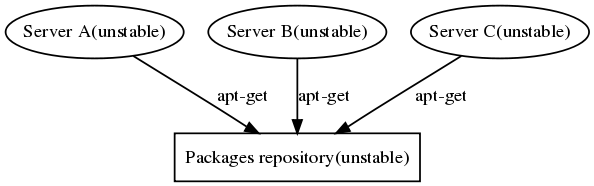
\includegraphics[width=10cm]{image200709/apt-proxy.png}
 \end{center}
 \end{figure}

 \begin{figure}[h]
 \begin{center}
$B;HMQ$7$?>l9g(B

 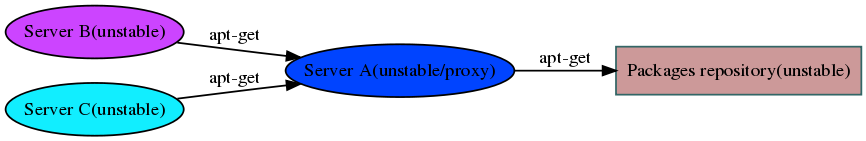
\includegraphics[width=15cm]{image200709/apt-proxy-e.png}
 \end{center}
 \end{figure}

%-------------------------
\subsection{$B%l%Y%k(B $BCf(B}
 $B0lHL%f!<%6!<$OCN$C$F$$$F$b$"$^$jLr$KN)$?$J$$$H;W$o$l$k(B apt-xxx$B!#(B
\subsubsection{apt-ftparchive}
 Sources.gz / Packages.gz $B$J$I$N%Q%C%1!<%8>pJsMQ%U%!%$%k$r:n@.$9$k$?$a$N%D!<%k!#(B
 $B<+J,$G:n$C$?%Q%C%1!<%8$r(B apt-line $B$H$7$F8x3+$7$?$$$H$-$K;H$$$^$9!#(B
\begin{commandline}
  % apt-ftparchive packages . | gzip -9 > Packages.gz 
  % apt-ftparchive sources . | gzip -9 > Sources.gz
  % apt-ftparchive release . > Release 
\end{commandline}

\subsubsection{apt-sortpkgs}
 Packages $B%U%!%$%k(B $B$*$h$S(B Sources $B%U%!%$%k$r%=!<%H$7$^$9!#(Bapt-ftparchive $B$G:n@.$7$?$b$N$O%=!<%H(B
 $B$5$l$F$$$J$+$C$?$j$9$k$N$G!"%"%k%U%!%Y%C%H=g$K%=!<%H$9$k$H$-$K;H$$$^$9!#(B
\begin{commandline}
 % apt-sortpkgs Packages > Packages.sort
\end{commandline} 

\subsubsection{apt-extracttemplates}
 Debian $B%Q%C%1!<%8$+$i@_Dj$H%F%s%W%l!<%H>pJs$rCj=P$9$k$?$a$N%D!<%k$G$9!#(B

\begin{commandline}
 % wget http://http.us.debian.org/debian/pool/main/x/xorg/xserver-xorg_7.3~rc1_all.deb
 % apt-extracttemplates xserver-xorg_7.3~rc1_all.deb
 % ls
 xserver-xorg.config.34261
 xserver-xorg.template.34260
\end{commandline}

\subsubsection{apt-build}
 Debian $B$GDs6!$5$l$F$$$k%P%$%J%j%Q%C%1!<%8$O$"$^$j:GE,2=$5$l$F$$$^$;$s!#(B
 $B?M$K$h$C$F$O<+J,$N4D6-$K9g$o$;$F%A%e!<%K%s%0$7$?$j!"@=IJ$KAH$_9~$s$@$j$9$k>l9g$b$"$j$^$9!#(B
 apt-build $B$O(B apt-get $B$9$k463P$G4D6-$K9g$o$;$F%P%$%J%j$r:n@.$r%5%]!<%H$9$k%D!<%k$G$9!#(B
 Debian $B%Q%C%1!<%8$r%j%S%k%I$9$k>l9g$O(B
 \begin{commandline}
 % apt-get update
 % apt-get source hello
 % cd hello-x.x
 % debuild -us -uc
 % sudo dpkg-i ../hello_xxxx.deb
 \end{commandline}
 $B$H$$$&<j=g$rF'$_$^$9$,!"(Bapt-build $B$N>l9g$O(B
 \begin{commandline}
 % apt-get update
 % apt-build install hello
 \end{commandline}
 $B$@$1$G$9!#(Bapt-build $B$N@_Dj%U%!%$%k$O(B
 \begin{commandline}
 /etc/apt/apt-build.conf
 \end{commandline}
 $B$K$"$j!"(B
 \begin{commandline}
build-dir = /var/cache/apt-build/build
repository-dir = /var/cache/apt-build/repository
Olevel = -O3
march = -march=pentium2
mcpu = -mcpu=pentium2
options =
 \end{commandline}
 $B$H$$$&@_Dj$K$J$C$F$$$^$9!#Nc$($P!"<+J,$N;H$C$F$$$k%^%7%s$,(B i686 $B$G$O$J$/!"(BCrusoe
 $B$N>l9g$K$O(B
\begin{commandline}
Olevel = 
-O2 -fomit-frame-pointer -fno-strict-aliasing -fno-common \ 
-pipe +-mpreferred-stack-boundary=2 -march=i686 -malign-functions=0 \
-malign-jumps=0 -malign-loops=0
\end{commandline}
$B$H$9$l$P$h$$$G$7$g$&!#(B

\subsubsection{apt-cross}
 Debian package $B$r(B cross$B4D6-$G;HMQ$G$-$k$h$&$KJQ49$7$F%$%s%9%H!<%k$7$F$^$9!#(B
 $B$$$^$^$G$O(B $B%@%&%s%m!<%I$7$?(B Debian package $B$r(B dpkg-cross $B$GJQ49$7$F(B
 $B%$%s%9%H!<%k$7$F$$$^$7$?$,!"(Bapt-cross $B$r;H$&$3$H$N$h$C$F!"<j:n6H$,8:$i$9$3$H$,(B
 $B$G$-$^$9!#(B

 \begin{figure}[h]
 \begin{center}
apt-cross $B$r;HMQ$7$J$$>l9g(B
 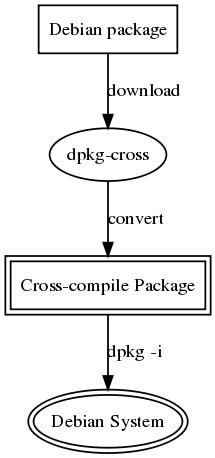
\includegraphics[width=16cm]{image200709/apt-cross.png}
 \end{center}
 \end{figure}

 \begin{figure}[h]
 \begin{center}
apt-cross $B$r;HMQ$7$?>l9g(B

 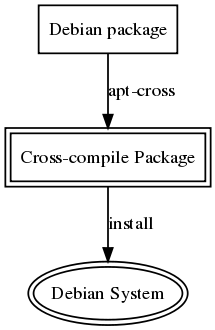
\includegraphics[width=12cm]{image200709/apt-cross-e.png}
 \end{center}
 \end{figure}

\subsubsection{apt-transport-https}
 apt $B$O(Bftp/http $B$G<hF@$G$-$k$N$G$9$,!"$3$N%Q%C%1!<%8$r;H$&$3$H$K$h$C$F(B
 https $B7PM3$G(B apt $B$r9T$&$3$H$,$G$-$k$h$&$K$J$j$^$9!#(B
%------------------------- 
\subsection{$B%l%Y%k(B $B9b(B}
 $BCN$C$F$$$F$b;H$o$J$$$@$m$&$H;W$o$l$k(B apt-xxx.
 $BOC$N%M%?$K$O$J$k$+$b$7$l$J$$!#(B
\subsubsection{apt-zip}
 $B%j%`!<%P%V%k%a%G%#%"$N(B ZIP $B$+$i$N(B apt $B$r%5%]!<%H$9$k$?$a$N%D!<%k$G$9!#(B
 $BF1$8$h$&$J%D!<%k$G(B apt-cdrom $B$,$"$j$^$9$,!"0c$$$,$$$^$$$A$o$+$j$^$;$s!#(B

\subsubsection{aptsh}
 apt $B$NA`:n$r$,$G$-$k(B Shell.
\begin{commandline}
 % sudo aptsh
\end{commandline} 
 $B$G(B shell$B$,(B aptsh $B$K$J$j$^$9!#;n$7$K!"(B
\begin{commandline}
 % ls
\end{commandline}
 $B$r<B9T$9$k$H!"%$%s%9%H!<%k2DG=$J%Q%C%1!<%80lMw$,I=<($5$l$^$9!#(B
 
\subsection{$B$^$H$a(B}
$B:#2s$O$5$o$j$@$1$r@bL@$7$^$7$?!#:#2s$N>R2p$G5$$K$J$k(Bapt-xxx $B$,$"$j$^$7$?$i(B
$B>\:Y$r@bL@$7$F$$$-$?$$$H;W$C$F$$$^$9!#(B

\dancersection{HP ML350G5 Debian etch $BF0:n3NG'(B}{$B>e@n(B $B=c0l(B}
\label{ml350g5}
\index{ML350G5}

\subsection{$B%5!<%P(B}

HP ML350G5 $B$O(B Intel Xeon CPU$B$rEk:\$7$F$$$k(B
Debian 4.0 (etch) $B$,2TF/$9$k$3$H$,%O!<%I%&%'%"%Y%s%@!"$*$h$S(BDebian$B%W%m%8%'(B
$B%/%H$NM-;V$K$h$C$F3NG'$5$l$F$$$k%5!<%P(B
\footnote{HP $B$N(B ProLiant $B$N(BDebian GNU/Linux $BBP1~%Z!<%8(B:
\url{http://www.hp.com/go/debian}}
\footnote{Debian $B$N(B ProLiant on Debian $B%Z!<%8(B:
\url{http://wiki.debian.org/HP/ProLiant}}
$B$G$9!#(B
$B:#2sMxMQ$7$?%5!<%P$K$O(B300GB$B$N(BSAS$B%G%#%9%/$,(B6$BK\Ek:\$5$l$F$$$^$7$?!#(B

\subsection{$B%$%s%9%H!<%kA0$N=`Hw(B}

$B%5!<%P$N5/F0;~$K!V(BF8$B!W$r2!$7!"(B
$B%O!<%I%&%'%"(BRAID$B5!G=$N@_Dj$r9T$$$^$9!#(B
$B:#2s$O0l$D$N(BRAID5$B$N%\%j%e!<%`(B($BLs(B1.5TB)$B$H$7$F(BOS$B$K8+$;$k@_Dj$K$7$^$7$?!#(B

\subsection{$B%$%s%9%H!<%k(B}

Debian installer $B$G%$%s%9%H!<%k$7$^$9!#:#2s$O(BDebian GNU/Linux 4.0r1 DVD 
$B$N(B1$BKgL\$rMxMQ$7$^$7$?!#(BML350G5 $B$O(B em64t $BBP1~$N(B Xeon $B$N$?$a!"(Bi386 $B$G$b(B 
amd64 $B$G$bF0:n$7$^$9!#:#2s$O(B amd64 $B$r%$%s%9%H!<%k$7$^$7$?!#(B

\subsection{$B%G%P%$%9$NG'<1(B}

$B3F<o%G%P%$%9$O4JC1$K2TF/$7$^$9!#(B
$B%0%i%U%#%C%/%+!<%I$O(B ati $B%I%i%$%P$GF0:n$7$^$9!#(B
debconf $B$G<+F0@_Dj$7$?CM$GE,@Z$J@_Dj%U%!%$%k$,=PNO$5$l$^$9!#(B

\begin{commandline}
# dpkg-reconfigure xserver-xorg
\end{commandline}

\subsection{USB $B%9%H%l!<%8%G%P%$%9$NG'<1(B}

$B<j85$K$"$C$?!V(BGreen house GH-UFD2GR$B!W$N(BUSB$B%a%b%j$GF0:n3NG'$7$?$H$3$m!"G'(B
$B<1$7$^$7$?!#(B

dmesg $B$O<!$N$h$&$K$J$j$^$7$?!'(B

\begin{commandline}
 usb 6-6: new high speed USB device using ehci_hcd and address 4
 usb 6-6: configuration #1 chosen from 1 choice
 Initializing USB Mass Storage driver...
 scsi0 : SCSI emulation for USB Mass Storage devices
 usbcore: registered new driver usb-storage
 USB Mass Storage support registered.
 usb-storage: device found at 4
 usb-storage: waiting for device to settle before scanning
  Vendor: USBDisk   Model: FlashDisk         Rev: 1.00
  Type:   Direct-Access                      ANSI SCSI revision: 02
 usb-storage: device scan complete
 SCSI device sda: 4005000 512-byte hdwr sectors (2051 MB)
 sda: Write Protect is off
 sda: Mode Sense: 0b 00 00 08
 sda: assuming drive cache: write through
 SCSI device sda: 4005000 512-byte hdwr sectors (2051 MB)
 sda: Write Protect is off
 sda: Mode Sense: 0b 00 00 08
 sda: assuming drive cache: write through
 sda: sda1
 sd 0:0:0:0: Attached scsi removable disk sda
 FAT: utf8 is not a recommended IO charset for FAT filesystems, filesystem will be case sensitive!
\end{commandline}


df $B$G3NG'$7$F$bG'<1$5$l$F$$$k$N$,$o$+$j$^$9!'(B

\begin{commandline}
# df -h /media/usbdisk/
Filesystem            Size  Used Avail Use% Mounted on
/dev/sda1             2.0G   76M  1.9G   4% /media/usbdisk
# df -T /media/usbdisk/
Filesystem    Type   1K-blocks      Used Available Use% Mounted on
/dev/sda1     vfat     2001888     76864   1925024   4% /media/usbdisk
\end{commandline}

\subsection{USB webcam $B$NG'<1(B}

PlayStation2 $BMQ(BUSB$B%+%a%i(B EyeToy $B$rF0:n$5$;$F$_$^$7$?!#(Bov51x-jpeg $B$N%G%P%$(B
$B%9%I%i%$%P$rG'<1$5$;$k$?$a$N%I%i%$%P$O;DG0$J$,$i(BDebian 4.0 $B$K$O4^$^$l$F$$(B
$B$J$$$N$G!":G?7$N%I%i%$%P$r%P%C%/%]!<%H$7$F$_$^$7$?!#(B

\begin{figure}[H]
\begin{center}
  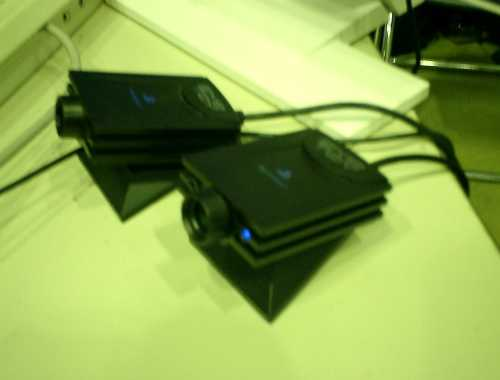
\includegraphics[width=0.5\hsize]{image200710/eyetoy.jpg}
\end{center}
\caption{EyeToy $B%+%a%i(B}
\label{eyetoy}
\end{figure}

%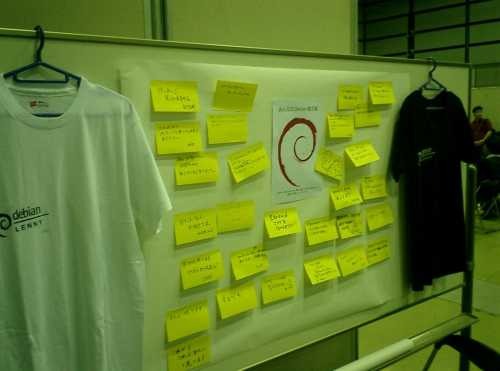
\includegraphics[width=0.5\hsize]{image200710/whiteboard.jpg}

$B$^$:!"%$%s%9%H!<%k$5$l$?%+!<%M%k$G%3%s%Q%$%k$9$k$?$a$KI,MW$J%Q%C%1!<%8$r(B
$B%$%s%9%H!<%k$7$^$9!#(B

\begin{commandline}
apt-get install linux-headers-2.6.18-5-amd64 linux-kbuild-2.6.18 \
 linux-source-2.6.18
\end{commandline}

ov51x-jpeg $B$N%=!<%9$r<hF@$7$F(B make $B%3%^%s%I$G%S%k%I$G$-$^$9!#(B

\begin{commandline}
debian:/home/hoge/ov51x-jpeg# make 
make -C /lib/modules/2.6.18-5-amd64/build M=/home/hoge/ov51x-jpeg modules
make[1]: Entering directory `/usr/src/linux-headers-2.6.18-5-amd64'
  CC [M]  /home/hoge/ov51x-jpeg/ov51x-jpeg-core.o
  CC [M]  /home/hoge/ov51x-jpeg/ov511-decomp.o
  CC [M]  /home/hoge/ov51x-jpeg/ov518-decomp.o
  CC [M]  /home/hoge/ov51x-jpeg/ov519-decomp.o
  LD [M]  /home/hoge/ov51x-jpeg/ov51x-jpeg.o
  Building modules, stage 2.
  MODPOST
  CC      /home/hoge/ov51x-jpeg/ov51x-jpeg.mod.o
  LD [M]  /home/hoge/ov51x-jpeg/ov51x-jpeg.ko
make[1]: Leaving directory `/usr/src/linux-headers-2.6.18-5-amd64'
 
\end{commandline}

$B@8@.$5$l$?%b%8%e!<%k$r$"$o$;$F(B insmod $B$9$l$P(B ekiga $B$G2hLL$,8+$l$k$h$&$K$J$j$^$9!#(B

\begin{commandline}
insmod v4l1-compat.ko
insmod v4l2-common.ko
insmod videodev.ko
insmod ov51x-jpeg.ko
\end{commandline}

\subsection{$B<U<-(B}

OSC Tokyo/Fall 2007 Debian $B%V!<%9$K$FK\:n6H$r9T$$$^$7$?!#(B
$B%5!<%P$OF|K\(BHP$B$+$i$*<Z$j$7$^$7$?!#(B

\begin{figure}[H]
\begin{center}
  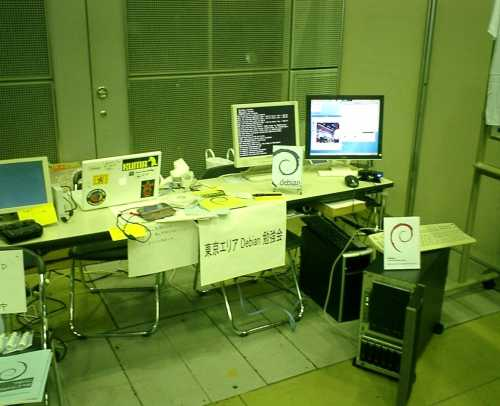
\includegraphics[width=0.5\hsize]{image200710/booth.jpg}
\end{center}
\caption{$B8!>Z;~$N%V!<%9$NMM;R(B}
\label{fig:oscfalldebbooth}
\end{figure}
\subsection{$BIUO?(B}

\subsubsection{dmesg}

$B5/F0;~$N(B dmesg $B$G$9!#(B

\begin{commandline}
Bootdata ok (command line is root=/dev/cciss/c0d0p1 ro )
Linux version 2.6.18-5-amd64 (Debian 2.6.18.dfsg.1-13) (dannf@debian.org) (gcc version 4.1.2 20061115 (prerelease) (Debian 4.1.1-21)) #1 SMP Thu May 31 23:51:05 UTC 2007
BIOS-provided physical RAM map:
 BIOS-e820: 0000000000000000 - 000000000009f400 (usable)
 BIOS-e820: 000000000009f400 - 00000000000a0000 (reserved)
 BIOS-e820: 00000000000f0000 - 0000000000100000 (reserved)
 BIOS-e820: 0000000000100000 - 000000003fe58000 (usable)
 BIOS-e820: 000000003fe58000 - 000000003fe60000 (ACPI data)
 BIOS-e820: 000000003fe60000 - 0000000040000000 (reserved)
 BIOS-e820: 00000000fec00000 - 00000000fed00000 (reserved)
 BIOS-e820: 00000000fee00000 - 00000000fee10000 (reserved)
 BIOS-e820: 00000000ffc00000 - 0000000100000000 (reserved)
DMI 2.3 present.
ACPI: RSDP (v002 HP                                    ) @ 0x00000000000f4f00
ACPI: XSDT (v001 HP     D21      0x00000002  0x0000162e) @ 0x000000003fe58300
ACPI: FADT (v003 HP     D21      0x00000002  0x0000162e) @ 0x000000003fe58380
ACPI: SPCR (v001 HP     SPCRRBSU 0x00000001  0x0000162e) @ 0x000000003fe58100
ACPI: MCFG (v001 HP     ProLiant 0x00000001  0x00000000) @ 0x000000003fe58180
ACPI: HPET (v001 HP     D21      0x00000002  0x0000162e) @ 0x000000003fe581c0
ACPI: SPMI (v005 HP     ProLiant 0x00000001  0x0000162e) @ 0x000000003fe58200
ACPI: MADT (v001 HP     00000083 0x00000002  0x00000000) @ 0x000000003fe58240
ACPI: DSDT (v001 HP         DSDT 0x00000001 INTL 0x20030228) @ 0x0000000000000000
No NUMA configuration found
Faking a node at 0000000000000000-000000003fe58000
Bootmem setup node 0 0000000000000000-000000003fe58000
On node 0 totalpages: 257159
  DMA zone: 3057 pages, LIFO batch:0
  DMA32 zone: 254102 pages, LIFO batch:31
ACPI: PM-Timer IO Port: 0x908
ACPI: Local APIC address 0xfee00000
ACPI: LAPIC (acpi_id[0x00] lapic_id[0x00] enabled)
Processor #0 6:15 APIC version 20
ACPI: LAPIC (acpi_id[0x04] lapic_id[0x04] disabled)
ACPI: LAPIC (acpi_id[0x02] lapic_id[0x02] disabled)
ACPI: LAPIC (acpi_id[0x06] lapic_id[0x06] disabled)
ACPI: LAPIC (acpi_id[0x01] lapic_id[0x01] enabled)
Processor #1 6:15 APIC version 20
ACPI: LAPIC (acpi_id[0x05] lapic_id[0x05] disabled)
ACPI: LAPIC (acpi_id[0x03] lapic_id[0x03] disabled)
ACPI: LAPIC (acpi_id[0x07] lapic_id[0x07] disabled)
ACPI: LAPIC_NMI (acpi_id[0xff] dfl dfl lint[0x1])
ACPI: IOAPIC (id[0x08] address[0xfec00000] gsi_base[0])
IOAPIC[0]: apic_id 8, version 32, address 0xfec00000, GSI 0-23
ACPI: IOAPIC (id[0x09] address[0xfec80000] gsi_base[24])
IOAPIC[1]: apic_id 9, version 32, address 0xfec80000, GSI 24-47
ACPI: INT_SRC_OVR (bus 0 bus_irq 0 global_irq 2 high edge)
ACPI: INT_SRC_OVR (bus 0 bus_irq 9 global_irq 9 high level)
ACPI: IRQ0 used by override.
ACPI: IRQ2 used by override.
ACPI: IRQ9 used by override.
Setting APIC routing to physical flat
ACPI: HPET id: 0x8086a201 base: 0xfed00000
Using ACPI (MADT) for SMP configuration information
Allocating PCI resources starting at 50000000 (gap: 40000000:bec00000)
SMP: Allowing 8 CPUs, 6 hotplug CPUs
Built 1 zonelists.  Total pages: 257159
Kernel command line: root=/dev/cciss/c0d0p1 ro 
Initializing CPU#0
PID hash table entries: 4096 (order: 12, 32768 bytes)
time.c: Using 14.318180 MHz WALL HPET GTOD HPET/TSC timer.
time.c: Detected 2666.763 MHz processor.
Console: colour VGA+ 80x25
Dentry cache hash table entries: 131072 (order: 8, 1048576 bytes)
Inode-cache hash table entries: 65536 (order: 7, 524288 bytes)
Checking aperture...
Memory: 1021852k/1046880k available (1927k kernel code, 24640k reserved, 868k data, 176k init)
Calibrating delay using timer specific routine.. 5338.29 BogoMIPS (lpj=10676592)
Security Framework v1.0.0 initialized
SELinux:  Disabled at boot.
Capability LSM initialized
Mount-cache hash table entries: 256
CPU: L1 I cache: 32K, L1 D cache: 32K
CPU: L2 cache: 4096K
using mwait in idle threads.
CPU: Physical Processor ID: 0
CPU: Processor Core ID: 0
CPU0: Thermal monitoring enabled (TM2)
SMP alternatives: switching to UP code
ACPI: Core revision 20060707
Using local APIC timer interrupts.
\end{commandline}
\begin{commandline}
result 20834085
Detected 20.834 MHz APIC timer.
SMP alternatives: switching to SMP code
Booting processor 1/2 APIC 0x1
Initializing CPU#1
Calibrating delay using timer specific routine.. 5333.44 BogoMIPS (lpj=10666883)
CPU: L1 I cache: 32K, L1 D cache: 32K
CPU: L2 cache: 4096K
CPU: Physical Processor ID: 0
CPU: Processor Core ID: 1
CPU1: Thermal monitoring enabled (TM2)
Intel(R) Xeon(R) CPU            5150  @ 2.66GHz stepping 06
Brought up 2 CPUs
testing NMI watchdog ... OK.
migration_cost=24
checking if image is initramfs... it is
Freeing initrd memory: 4896k freed
NET: Registered protocol family 16
ACPI: bus type pci registered
PCI: BIOS Bug: MCFG area at e0000000 is not E820-reserved
PCI: Not using MMCONFIG.
PCI: Using configuration type 1
ACPI: Interpreter enabled
ACPI: Using IOAPIC for interrupt routing
ACPI: PCI Root Bridge [PCI0] (0000:00)
PCI: Probing PCI hardware (bus 00)
ACPI: Assume root bridge [\_SB_.PCI0] bus is 0
PCI: Ignoring BAR0-3 of IDE controller 0000:00:1f.1
Boot video device is 0000:01:03.0
PCI: Transparent bridge - 0000:00:1e.0
ACPI: PCI Interrupt Routing Table [\_SB_.PCI0._PRT]
ACPI: PCI Interrupt Routing Table [\_SB_.PCI0.IP2P._PRT]
ACPI: PCI Interrupt Routing Table [\_SB_.PCI0.IPTA._PRT]
ACPI: PCI Interrupt Routing Table [\_SB_.PCI0.PT02._PRT]
ACPI: PCI Interrupt Routing Table [\_SB_.PCI0.PT02.PEX2._PRT]
ACPI: PCI Interrupt Routing Table [\_SB_.PCI0.PT02.IPE4._PRT]
ACPI: PCI Interrupt Routing Table [\_SB_.PCI0.PT02.IPE4.IPE1._PRT]
ACPI: PCI Interrupt Routing Table [\_SB_.PCI0.PT02.IPE4.IPE2._PRT]
ACPI: PCI Interrupt Routing Table [\_SB_.PCI0.PT04._PRT]
ACPI: PCI Interrupt Routing Table [\_SB_.PCI0.PT05.EEPB._PRT]
ACPI: PCI Interrupt Routing Table [\_SB_.PCI0.PT05.EEPB.EPPB._PRT]
ACPI: PCI Interrupt Link [LNKA] (IRQs *5 7 10 11)
ACPI: PCI Interrupt Link [LNKB] (IRQs 5 *7 10 11)
ACPI: PCI Interrupt Link [LNKC] (IRQs 5 7 *10 11)
ACPI: PCI Interrupt Link [LNKD] (IRQs 5 7 *10 11)
ACPI: PCI Interrupt Link [LNKE] (IRQs 5 7 10 11) *0, disabled.
ACPI: PCI Interrupt Link [LNKF] (IRQs *5 7 10 11)
ACPI: PCI Interrupt Link [LNKG] (IRQs 5 7 *10 11)
ACPI: PCI Interrupt Link [LNKH] (IRQs 5 *7 10 11)
Linux Plug and Play Support v0.97 (c) Adam Belay
pnp: PnP ACPI init
pnp: ACPI device : hid PNP0A03
pnp: ACPI device : hid PNP0C02
pnp: ACPI device : hid IPI0001
pnp: ACPI device : hid PNP0103
pnp: ACPI device : hid PNP0200
pnp: ACPI device : hid PNP0800
pnp: ACPI device : hid PNP0303
pnp: ACPI device : hid PNP0F13
pnp: ACPI device : hid PNP0A06
pnp: ACPI device : hid PNP0501
pnp: ACPI device : hid PNP0700
pnp: PnP ACPI: found 11 devices
usbcore: registered new driver usbfs
usbcore: registered new driver hub
PCI: Using ACPI for IRQ routing
PCI: If a device doesn't work, try "pci=routeirq".  If it helps, post a report
hpet0: at MMIO 0xfed00000 (virtual 0xffffffffff5fe000), IRQs 2, 8, 0
hpet0: 3 64-bit timers, 14318180 Hz
PCI-GART: No AMD northbridge found.
pnp: the driver 'system' has been registered
pnp: match found with the PnP device '00:01' and the driver 'system'
pnp: 00:01: ioport range 0x408-0x40f has been reserved
pnp: 00:01: ioport range 0x4d0-0x4d1 has been reserved
pnp: 00:01: ioport range 0x700-0x71f has been reserved
PCI: Bridge: 0000:05:00.0
  IO window: disabled.
  MEM window: disabled.
  PREFETCH window: disabled.
PCI: Bridge: 0000:05:01.0
  IO window: disabled.
  MEM window: disabled.
  PREFETCH window: disabled.
PCI: Bridge: 0000:04:00.0
  IO window: disabled.
  MEM window: disabled.
  PREFETCH window: disabled.
PCI: Bridge: 0000:04:00.3
  IO window: disabled.
  MEM window: disabled.
  PREFETCH window: disabled.
PCI: Bridge: 0000:00:02.0
  IO window: disabled.
  MEM window: fde00000-fdefffff
  PREFETCH window: disabled.
\end{commandline}
\begin{commandline}
PCI: Bridge: 0000:00:03.0
  IO window: disabled.
  MEM window: disabled.
  PREFETCH window: disabled.
PCI: Bridge: 0000:00:04.0
  IO window: disabled.
  MEM window: disabled.
  PREFETCH window: disabled.
PCI: Bridge: 0000:13:04.0
  IO window: disabled.
  MEM window: disabled.
  PREFETCH window: disabled.
PCI: Bridge: 0000:12:00.0
  IO window: 4000-4fff
  MEM window: fdf00000-fdffffff
  PREFETCH window: 50000000-500fffff
PCI: Bridge: 0000:00:05.0
  IO window: 4000-4fff
  MEM window: fdf00000-fdffffff
  PREFETCH window: 50000000-500fffff
PCI: Bridge: 0000:02:00.0
  IO window: disabled.
  MEM window: fa000000-fbffffff
  PREFETCH window: 50100000-501fffff
PCI: Bridge: 0000:00:1c.0
  IO window: disabled.
  MEM window: fa000000-fbffffff
  PREFETCH window: 50100000-501fffff
PCI: Bridge: 0000:00:1e.0
  IO window: 2000-3fff
  MEM window: f9e00000-f9ffffff
  PREFETCH window: f0000000-f7ffffff
PCI: Setting latency timer of device 0000:00:02.0 to 64
PCI: Setting latency timer of device 0000:04:00.0 to 64
GSI 16 sharing vector 0xA9 and IRQ 16
ACPI: PCI Interrupt 0000:05:00.0[A] -> GSI 16 (level, low) -> IRQ 169
PCI: Setting latency timer of device 0000:05:00.0 to 64
GSI 17 sharing vector 0xB1 and IRQ 17
ACPI: PCI Interrupt 0000:05:01.0[A] -> GSI 17 (level, low) -> IRQ 177
PCI: Setting latency timer of device 0000:05:01.0 to 64
PCI: Setting latency timer of device 0000:04:00.3 to 64
PCI: Setting latency timer of device 0000:00:03.0 to 64
PCI: Setting latency timer of device 0000:00:04.0 to 64
PCI: Setting latency timer of device 0000:00:05.0 to 64
PCI: Setting latency timer of device 0000:12:00.0 to 64
ACPI: PCI Interrupt 0000:00:1c.0[A] -> GSI 16 (level, low) -> IRQ 169
PCI: Setting latency timer of device 0000:00:1c.0 to 64
PCI: Setting latency timer of device 0000:02:00.0 to 64
PCI: Setting latency timer of device 0000:00:1e.0 to 64
NET: Registered protocol family 2
IP route cache hash table entries: 32768 (order: 6, 262144 bytes)
TCP established hash table entries: 131072 (order: 9, 2097152 bytes)
TCP bind hash table entries: 65536 (order: 8, 1048576 bytes)
TCP: Hash tables configured (established 131072 bind 65536)
TCP reno registered
audit: initializing netlink socket (disabled)
audit(1186902200.772:1): initialized
VFS: Disk quotas dquot_6.5.1
Dquot-cache hash table entries: 512 (order 0, 4096 bytes)
Initializing Cryptographic API
io scheduler noop registered
io scheduler anticipatory registered
io scheduler deadline registered
io scheduler cfq registered (default)
PCI: Setting latency timer of device 0000:00:02.0 to 64
pcie_portdrv_probe->Dev[25f7:8086] has invalid IRQ. Check vendor BIOS
assign_interrupt_mode Found MSI capability
Allocate Port Service[0000:00:02.0:pcie00]
PCI: Setting latency timer of device 0000:00:03.0 to 64
pcie_portdrv_probe->Dev[25e3:8086] has invalid IRQ. Check vendor BIOS
assign_interrupt_mode Found MSI capability
Allocate Port Service[0000:00:03.0:pcie00]
PCI: Setting latency timer of device 0000:00:04.0 to 64
pcie_portdrv_probe->Dev[25e4:8086] has invalid IRQ. Check vendor BIOS
assign_interrupt_mode Found MSI capability
Allocate Port Service[0000:00:04.0:pcie00]
PCI: Setting latency timer of device 0000:00:05.0 to 64
pcie_portdrv_probe->Dev[25e5:8086] has invalid IRQ. Check vendor BIOS
assign_interrupt_mode Found MSI capability
Allocate Port Service[0000:00:05.0:pcie00]
PCI: Setting latency timer of device 0000:00:1c.0 to 64
assign_interrupt_mode Found MSI capability
Allocate Port Service[0000:00:1c.0:pcie00]
PCI: Setting latency timer of device 0000:04:00.0 to 64
pcie_portdrv_probe->Dev[3500:8086] has invalid IRQ. Check vendor BIOS
Allocate Port Service[0000:04:00.0:pcie10]
PCI: Setting latency timer of device 0000:05:00.0 to 64
assign_interrupt_mode Found MSI capability
Allocate Port Service[0000:05:00.0:pcie20]
PCI: Setting latency timer of device 0000:05:01.0 to 64
assign_interrupt_mode Found MSI capability
Allocate Port Service[0000:05:01.0:pcie20]
Real Time Clock Driver v1.12ac
hpet_resources: 0xfed00000 is busy
\end{commandline}
\begin{commandline}
Linux agpgart interface v0.101 (c) Dave Jones
Serial: 8250/16550 driver $Revision: 1.90 $ 4 ports, IRQ sharing enabled
serial8250: ttyS0 at I/O 0x3f8 (irq = 4) is a 16550A
serial8250: ttyS1 at I/O 0x2f8 (irq = 3) is a 16550A
pnp: the driver 'serial' has been registered
pnp: match found with the PnP device '00:09' and the driver 'serial'
00:09: ttyS0 at I/O 0x3f8 (irq = 4) is a 16550A
RAMDISK driver initialized: 16 RAM disks of 65536K size 1024 blocksize
pnp: the driver 'i8042 kbd' has been registered
pnp: match found with the PnP device '00:06' and the driver 'i8042 kbd'
pnp: the driver 'i8042 aux' has been registered
pnp: match found with the PnP device '00:07' and the driver 'i8042 aux'
PNP: PS/2 Controller [PNP0303:KBD,PNP0f0e:PS2M] at 0x60,0x64 irq 1,12
serio: i8042 AUX port at 0x60,0x64 irq 12
serio: i8042 KBD port at 0x60,0x64 irq 1
mice: PS/2 mouse device common for all mice
TCP bic registered
NET: Registered protocol family 1
NET: Registered protocol family 17
NET: Registered protocol family 8
NET: Registered protocol family 20
ACPI: (supports S0 S4 S5)
Freeing unused kernel memory: 176k freed
ACPI Exception (acpi_processor-0681): AE_NOT_FOUND, Processor Device is not present [20060707]
ACPI: Getting cpuindex for acpiid 0x2
ACPI Exception (acpi_processor-0681): AE_NOT_FOUND, Processor Device is not present [20060707]
ACPI: Getting cpuindex for acpiid 0x3
ACPI Exception (acpi_processor-0681): AE_NOT_FOUND, Processor Device is not present [20060707]
ACPI: Getting cpuindex for acpiid 0x4
ACPI Exception (acpi_processor-0681): AE_NOT_FOUND, Processor Device is not present [20060707]
ACPI: Getting cpuindex for acpiid 0x5
ACPI Exception (acpi_processor-0681): AE_NOT_FOUND, Processor Device is not present [20060707]
ACPI: Getting cpuindex for acpiid 0x6
ACPI Exception (acpi_processor-0681): AE_NOT_FOUND, Processor Device is not present [20060707]
ACPI: Getting cpuindex for acpiid 0x7
ACPI: Thermal Zone [THM0] (8 C)
input: AT Translated Set 2 keyboard as /class/input/input0
USB Universal Host Controller Interface driver v3.0
ACPI: PCI Interrupt 0000:00:1d.0[A] -> GSI 16 (level, low) -> IRQ 169
PCI: Setting latency timer of device 0000:00:1d.0 to 64
uhci_hcd 0000:00:1d.0: UHCI Host Controller
uhci_hcd 0000:00:1d.0: new USB bus registered, assigned bus number 1
uhci_hcd 0000:00:1d.0: irq 169, io base 0x00001000
usb usb1: configuration #1 chosen from 1 choice
hub 1-0:1.0: USB hub found
hub 1-0:1.0: 2 ports detected
SCSI subsystem initialized
HP CISS Driver (v 3.6.10)
Uniform Multi-Platform E-IDE driver Revision: 7.00alpha2
ide: Assuming 33MHz system bus speed for PIO modes; override with idebus=xx
ACPI: PCI Interrupt 0000:00:1d.1[B] -> GSI 17 (level, low) -> IRQ 177
PCI: Setting latency timer of device 0000:00:1d.1 to 64
uhci_hcd 0000:00:1d.1: UHCI Host Controller
uhci_hcd 0000:00:1d.1: new USB bus registered, assigned bus number 2
uhci_hcd 0000:00:1d.1: irq 177, io base 0x00001020
usb usb2: configuration #1 chosen from 1 choice
hub 2-0:1.0: USB hub found
hub 2-0:1.0: 2 ports detected
GSI 18 sharing vector 0x3A and IRQ 18
ACPI: PCI Interrupt 0000:00:1d.2[C] -> GSI 18 (level, low) -> IRQ 58
PCI: Setting latency timer of device 0000:00:1d.2 to 64
uhci_hcd 0000:00:1d.2: UHCI Host Controller
uhci_hcd 0000:00:1d.2: new USB bus registered, assigned bus number 3
uhci_hcd 0000:00:1d.2: irq 58, io base 0x00001040
usb usb3: configuration #1 chosen from 1 choice
hub 3-0:1.0: USB hub found
hub 3-0:1.0: 2 ports detected
GSI 19 sharing vector 0x42 and IRQ 19
ACPI: PCI Interrupt 0000:00:1d.3[D] -> GSI 19 (level, low) -> IRQ 66
PCI: Setting latency timer of device 0000:00:1d.3 to 64
uhci_hcd 0000:00:1d.3: UHCI Host Controller
uhci_hcd 0000:00:1d.3: new USB bus registered, assigned bus number 4
uhci_hcd 0000:00:1d.3: irq 66, io base 0x00001060
usb usb4: configuration #1 chosen from 1 choice
hub 4-0:1.0: USB hub found
hub 4-0:1.0: 2 ports detected
Broadcom NetXtreme II Gigabit Ethernet Driver bnx2 v1.4.44 (August 10, 2006)
ACPI: PCI Interrupt 0000:03:00.0[A] -> GSI 16 (level, low) -> IRQ 169
eth0: Broadcom NetXtreme II BCM5708 1000Base-T (B2) PCI-X 64-bit 133MHz found at mem fa000000, IRQ 169, node addr 001b7873259a
GSI 20 sharing vector 0x4A and IRQ 20
ACPI: PCI Interrupt 0000:01:04.4[B] -> GSI 22 (level, low) -> IRQ 74
uhci_hcd 0000:01:04.4: UHCI Host Controller
uhci_hcd 0000:01:04.4: new USB bus registered, assigned bus number 5
uhci_hcd 0000:01:04.4: port count misdetected? forcing to 2 ports
uhci_hcd 0000:01:04.4: irq 74, io base 0x00003800
usb usb5: configuration #1 chosen from 1 choice
hub 5-0:1.0: USB hub found
hub 5-0:1.0: 2 ports detected
\end{commandline}
\begin{commandline}
ESB2: IDE controller at PCI slot 0000:00:1f.1
ACPI: Unable to derive IRQ for device 0000:00:1f.1
ACPI: PCI Interrupt 0000:00:1f.1[A]: no GSI - using IRQ 7
ESB2: chipset revision 9
ESB2: not 100% native mode: will probe irqs later
    ide0: BM-DMA at 0x0500-0x0507, BIOS settings: hda:DMA, hdb:pio
    ide1: BM-DMA at 0x0508-0x050f, BIOS settings: hdc:pio, hdd:pio
Probing IDE interface ide0...
usb 5-1: new full speed USB device using uhci_hcd and address 2
usb 5-1: configuration #1 chosen from 1 choice
usb 5-2: new full speed USB device using uhci_hcd and address 3
hda: HL-DT-STDVD+-RW GSA-H21L, ATAPI CD/DVD-ROM drive
usb 5-2: configuration #1 chosen from 1 choice
hub 5-2:1.0: USB hub found
hub 5-2:1.0: 7 ports detected
usbcore: registered new driver hiddev
input: HP Virtual Keyboard as /class/input/input1
input: USB HID v1.01 Keyboard [HP Virtual Keyboard] on usb-0000:01:04.4-1
input: HP Virtual Keyboard as /class/input/input2
input: USB HID v1.01 Mouse [HP Virtual Keyboard] on usb-0000:01:04.4-1
usbcore: registered new driver usbhid
drivers/usb/input/hid-core.c: v2.6:USB HID core driver
ide0 at 0x1f0-0x1f7,0x3f6 on irq 14
Probing IDE interface ide1...
ACPI: PCI Interrupt 0000:00:1d.7[A] -> GSI 16 (level, low) -> IRQ 169
PCI: Setting latency timer of device 0000:00:1d.7 to 64
ehci_hcd 0000:00:1d.7: EHCI Host Controller
ehci_hcd 0000:00:1d.7: new USB bus registered, assigned bus number 6
ehci_hcd 0000:00:1d.7: debug port 1
PCI: cache line size of 32 is not supported by device 0000:00:1d.7
ehci_hcd 0000:00:1d.7: irq 169, io mem 0xf9df0000
ehci_hcd 0000:00:1d.7: USB 2.0 started, EHCI 1.00, driver 10 Dec 2004
usb usb6: configuration #1 chosen from 1 choice
hub 6-0:1.0: USB hub found
hub 6-0:1.0: 8 ports detected
ACPI: PCI Interrupt 0000:13:08.0[A] -> GSI 19 (level, low) -> IRQ 66
cciss0: <0x3238> at PCI 0000:13:08.0 IRQ 82 using DAC
      blocks= 2929359452 block_size= 512
      heads= 255, sectors= 32, cylinders= 358991

      blocks= 2929359452 block_size= 512
      heads= 255, sectors= 32, cylinders= 358991

 cciss/c0d0: p1 p2 < p5 >
hda: ATAPI 48X DVD-ROM DVD-R CD-R/RW drive, 2048kB Cache, UDMA(33)
Uniform CD-ROM driver Revision: 3.20
Attempting manual resume
kjournald starting.  Commit interval 5 seconds
EXT3-fs: mounted filesystem with ordered data mode.
pci_hotplug: PCI Hot Plug PCI Core version: 0.5
shpchp: Standard Hot Plug PCI Controller Driver version: 0.4
intel_rng: FWH not detected
input: PC Speaker as /class/input/input3
Floppy drive(s): fd0 is 1.44M
floppy0: no floppy controllers found
Adding 3004112k swap on /dev/cciss/c0d0p5.  Priority:-1 extents:1 across:3004112k
EXT3 FS on cciss/c0d0p1, internal journal
loop: loaded (max 8 devices)
device-mapper: ioctl: 4.7.0-ioctl (2006-06-24) initialised: dm-devel@redhat.com
ACPI: Power Button (FF) [PWRF]
\end{commandline}

\subsubsection{$B%G%P%$%9@\B3(B}

\begin{commandline}
# lspci 
00:00.0 Host bridge: Intel Corporation 5000Z Chipset Memory Controller Hub (rev b1)
00:02.0 PCI bridge: Intel Corporation 5000 Series Chipset PCI Express x8 Port 2-3 (rev b1)
00:03.0 PCI bridge: Intel Corporation 5000 Series Chipset PCI Express x4 Port 3 (rev b1)
00:04.0 PCI bridge: Intel Corporation 5000 Series Chipset PCI Express x4 Port 4 (rev b1)
00:05.0 PCI bridge: Intel Corporation 5000 Series Chipset PCI Express x4 Port 5 (rev b1)
00:10.0 Host bridge: Intel Corporation 5000 Series Chipset Error Reporting Registers (rev b1)
00:10.1 Host bridge: Intel Corporation 5000 Series Chipset Error Reporting Registers (rev b1)
00:10.2 Host bridge: Intel Corporation 5000 Series Chipset Error Reporting Registers (rev b1)
00:11.0 Host bridge: Intel Corporation 5000 Series Chipset Reserved Registers (rev b1)
00:13.0 Host bridge: Intel Corporation 5000 Series Chipset Reserved Registers (rev b1)
00:15.0 Host bridge: Intel Corporation 5000 Series Chipset FBD Registers (rev b1)
00:16.0 Host bridge: Intel Corporation 5000 Series Chipset FBD Registers (rev b1)
00:1c.0 PCI bridge: Intel Corporation 631xESB/632xESB/3100 Chipset PCI Express Root Port 1 (rev 09)
00:1d.0 USB Controller: Intel Corporation 631xESB/632xESB/3100 Chipset UHCI USB Controller #1 (rev 09)
00:1d.1 USB Controller: Intel Corporation 631xESB/632xESB/3100 Chipset UHCI USB Controller #2 (rev 09)
00:1d.2 USB Controller: Intel Corporation 631xESB/632xESB/3100 Chipset UHCI USB Controller #3 (rev 09)
00:1d.3 USB Controller: Intel Corporation 631xESB/632xESB/3100 Chipset UHCI USB Controller #4 (rev 09)
00:1d.7 USB Controller: Intel Corporation 631xESB/632xESB/3100 Chipset EHCI USB2 Controller (rev 09)
00:1e.0 PCI bridge: Intel Corporation 82801 PCI Bridge (rev d9)
00:1f.0 ISA bridge: Intel Corporation 631xESB/632xESB/3100 Chipset LPC Interface Controller (rev 09)
00:1f.1 IDE interface: Intel Corporation 631xESB/632xESB IDE Controller (rev 09)
01:03.0 VGA compatible controller: ATI Technologies Inc ES1000 (rev 02)
01:04.0 System peripheral: Compaq Computer Corporation Integrated Lights Out Controller (rev 03)
01:04.2 System peripheral: Compaq Computer Corporation Integrated Lights Out  Processor (rev 03)
01:04.4 USB Controller: Hewlett-Packard Company Unknown device 3300
01:04.6 Serial bus controller [0c07]: Hewlett-Packard Company Unknown device 3302
02:00.0 PCI bridge: Broadcom EPB PCI-Express to PCI-X Bridge (rev c3)
03:00.0 Ethernet controller: Broadcom Corporation NetXtreme II BCM5708 Gigabit Ethernet (rev 12)
04:00.0 PCI bridge: Intel Corporation 6311ESB/6321ESB PCI Express Upstream Port (rev 01)
04:00.3 PCI bridge: Intel Corporation 6311ESB/6321ESB PCI Express to PCI-X Bridge (rev 01)
05:00.0 PCI bridge: Intel Corporation 6311ESB/6321ESB PCI Express Downstream Port E1 (rev 01)
05:01.0 PCI bridge: Intel Corporation 6311ESB/6321ESB PCI Express Downstream Port E2 (rev 01)
12:00.0 PCI bridge: Broadcom EPB PCI-Express to PCI-X Bridge (rev b4)
13:04.0 PCI bridge: Broadcom HT1000 PCI/PCI-X bridge (rev b2)
13:08.0 RAID bus controller: Hewlett-Packard Company Unknown device 3238

# lspci -n 
00:00.0 0600: 8086:25d0 (rev b1)
00:02.0 0604: 8086:25f7 (rev b1)
00:03.0 0604: 8086:25e3 (rev b1)
00:04.0 0604: 8086:25e4 (rev b1)
00:05.0 0604: 8086:25e5 (rev b1)
00:10.0 0600: 8086:25f0 (rev b1)
00:10.1 0600: 8086:25f0 (rev b1)
00:10.2 0600: 8086:25f0 (rev b1)
00:11.0 0600: 8086:25f1 (rev b1)
00:13.0 0600: 8086:25f3 (rev b1)
00:15.0 0600: 8086:25f5 (rev b1)
00:16.0 0600: 8086:25f6 (rev b1)
00:1c.0 0604: 8086:2690 (rev 09)
00:1d.0 0c03: 8086:2688 (rev 09)
00:1d.1 0c03: 8086:2689 (rev 09)
00:1d.2 0c03: 8086:268a (rev 09)
00:1d.3 0c03: 8086:268b (rev 09)
00:1d.7 0c03: 8086:268c (rev 09)
00:1e.0 0604: 8086:244e (rev d9)
00:1f.0 0601: 8086:2670 (rev 09)
00:1f.1 0101: 8086:269e (rev 09)
01:03.0 0300: 1002:515e (rev 02)
01:04.0 0880: 0e11:b203 (rev 03)
01:04.2 0880: 0e11:b204 (rev 03)
01:04.4 0c03: 103c:3300
01:04.6 0c07: 103c:3302
02:00.0 0604: 1166:0103 (rev c3)
03:00.0 0200: 14e4:164c (rev 12)
04:00.0 0604: 8086:3500 (rev 01)
04:00.3 0604: 8086:350c (rev 01)
05:00.0 0604: 8086:3510 (rev 01)
05:01.0 0604: 8086:3514 (rev 01)
12:00.0 0604: 1166:0103 (rev b4)
13:04.0 0604: 1166:0104 (rev b2)
13:08.0 0104: 103c:3238
\end{commandline}

\subsubsection{lshw $B$N=PNO(B}

\begin{commandline}
# lshw 
debian
    description: Computer
    product: ProLiant ML350 G5
    vendor: HP
    serial: CN7719011K
    width: 32 bits
    capabilities: smbios-2.3 dmi-2.3
    configuration: boot=hardware-failure-fw uuid=41473538-3641-434E-3737-31393031314B
  *-core
       description: Motherboard
       physical id: 0
     *-firmware
          description: BIOS
          vendor: HP
          physical id: 0
          version: D21 (04/06/2007)
          size: 64KB
          capacity: 4032KB
          capabilities: pci pnp upgrade shadowing escd cdboot bootselect int13floppy360 int13floppy1200 int13floppy720 int5printscreen int9keyboard int14serial int17printer int10video acpi usb biosbootspecification
     *-cpu:0
          description: CPU
          product: Intel(R) Xeon(R) CPU            5150  @ 2.66GHz
          vendor: Intel Corp.
          physical id: 400
          bus info: cpu@0
          slot: Proc 1
          size: 2666MHz
          width: 64 bits
          clock: 1333MHz
          capabilities: fpu fpu_exception wp vme de pse tsc msr pae mce cx8 apic sep mtrr pge mca cmov pat pse36 clflush dts acpi mmx fxsr sse sse2 ss ht tm syscall x86-64 constant_tsc pni monitor ds_cpl vmx est tm2 cx16 xtpr lahf_lm
        *-cache:0
             description: L1 cache
             physical id: 710
             slot: Processor 1 Internal L1 Cache
             size: 64KB
             capacity: 128KB
             capabilities: burst internal write-back data
        *-cache:1
             description: L2 cache
             physical id: 720
             slot: Processor 1 Internal L2 Cache
             size: 4MB
             capacity: 16MB
             capabilities: burst internal write-back
        *-cache:2 DISABLED
             description: L3 cache
             physical id: 730
             slot: Processor 1 Internal L3 Cache
             capacity: 8MB
             capabilities: burst internal
     *-cpu:1
          description: CPU
          vendor: Intel
          physical id: 406
          bus info: cpu@1
          slot: Proc 2
          capacity: 505MHz
          clock: 200MHz
        *-cache:0 DISABLED
             description: L1 cache
             physical id: 716
             slot: Processor 2 Internal L1 Cache
             capacity: 128KB
             capabilities: burst internal data
        *-cache:1 DISABLED
             description: L2 cache
             physical id: 726
             slot: Processor 2 Internal L2 Cache
             capacity: 16MB
             capabilities: burst internal
        *-cache:2 DISABLED
             description: L3 cache
             physical id: 736
             slot: Processor 2 Internal L3 Cache
             capacity: 8MB
             capabilities: burst internal
\end{commandline}
\begin{commandline}
     *-memory
          description: System Memory
          physical id: 1000
          slot: System board or motherboard
          size: 1GB
        *-bank:0
             description: Synchronous 667 MHz (1.5 ns)
             physical id: 0
             slot: DIMM 1A
             size: 512MB
             width: 64 bits
             clock: 667MHz (1.5ns)
        *-bank:1
             description: Synchronous [empty]
             physical id: 1
             slot: DIMM 2B
             width: 64 bits
        *-bank:2
             description: Synchronous [empty]
             physical id: 2
             slot: DIMM 3C
             width: 64 bits
        *-bank:3
             description: Synchronous [empty]
             physical id: 3
             slot: DIMM 4D
             width: 64 bits
        *-bank:4
             description: Synchronous 667 MHz (1.5 ns)
             physical id: 4
             slot: DIMM 5A
             size: 512MB
             width: 64 bits
             clock: 667MHz (1.5ns)
        *-bank:5
             description: Synchronous [empty]
             physical id: 5
             slot: DIMM 6B
             width: 64 bits
        *-bank:6
             description: Synchronous [empty]
             physical id: 6
             slot: DIMM 7C
             width: 64 bits
        *-bank:7
             description: Synchronous [empty]
             physical id: 7
             slot: DIMM 8D
             width: 64 bits
     *-pci:0
          description: Host bridge
          product: 5000Z Chipset Memory Controller Hub
          vendor: Intel Corporation
          physical id: 100
          bus info: pci@00:00.0
          version: b1
          width: 32 bits
          clock: 33MHz
        *-pci:0
             description: PCI bridge
             product: 5000 Series Chipset PCI Express x8 Port 2-3
             vendor: Intel Corporation
             physical id: 2
             bus info: pci@00:02.0
             version: b1
             width: 32 bits
             clock: 33MHz
             capabilities: pci normal_decode bus_master cap_list
             configuration: driver=pcieport-driver
           *-pci:0
                description: PCI bridge
                product: 6311ESB/6321ESB PCI Express Upstream Port
                vendor: Intel Corporation
                physical id: 0
                bus info: pci@04:00.0
                version: 01
                width: 64 bits
                clock: 33MHz
                capabilities: pci normal_decode bus_master cap_list
                configuration: driver=pcieport-driver
                resources: iomemory:200000f00-200000eff
              *-pci:0
                   description: PCI bridge
                   product: 6311ESB/6321ESB PCI Express Downstream Port E1
                   vendor: Intel Corporation
                   physical id: 0
                   bus info: pci@05:00.0
                   version: 01
                   width: 32 bits
                   clock: 33MHz
                   capabilities: pci normal_decode bus_master cap_list
                   configuration: driver=pcieport-driver
              *-pci:1
                   description: PCI bridge
                   product: 6311ESB/6321ESB PCI Express Downstream Port E2
                   vendor: Intel Corporation
                   physical id: 1
                   bus info: pci@05:01.0
                   version: 01
                   width: 32 bits
                   clock: 33MHz
                   capabilities: pci normal_decode bus_master cap_list
                   configuration: driver=pcieport-driver
\end{commandline}
\begin{commandline}
           *-pci:1
                description: PCI bridge
                product: 6311ESB/6321ESB PCI Express to PCI-X Bridge
                vendor: Intel Corporation
                physical id: 0.3
                bus info: pci@04:00.3
                version: 01
                width: 64 bits
                clock: 33MHz
                capabilities: pci normal_decode bus_master cap_list
                resources: iomemory:22a000f00-22a000eff
        *-pci:1
             description: PCI bridge
             product: 5000 Series Chipset PCI Express x4 Port 3
             vendor: Intel Corporation
             physical id: 3
             bus info: pci@00:03.0
             version: b1
             width: 32 bits
             clock: 33MHz
             capabilities: pci normal_decode bus_master cap_list
             configuration: driver=pcieport-driver
        *-pci:2
             description: PCI bridge
             product: 5000 Series Chipset PCI Express x4 Port 4
             vendor: Intel Corporation
             physical id: 4
             bus info: pci@00:04.0
             version: b1
             width: 32 bits
             clock: 33MHz
             capabilities: pci normal_decode bus_master cap_list
             configuration: driver=pcieport-driver
        *-pci:3
             description: PCI bridge
             product: 5000 Series Chipset PCI Express x4 Port 5
             vendor: Intel Corporation
             physical id: 5
             bus info: pci@00:05.0
             version: b1
             width: 32 bits
             clock: 33MHz
             capabilities: pci normal_decode bus_master cap_list
             configuration: driver=pcieport-driver
           *-pci
                description: PCI bridge
                product: EPB PCI-Express to PCI-X Bridge
                vendor: Broadcom
                physical id: 0
                bus info: pci@12:00.0
                version: b4
                width: 32 bits
                clock: 33MHz
                capabilities: pci normal_decode bus_master cap_list
              *-pci
                   description: PCI bridge
                   product: HT1000 PCI/PCI-X bridge
                   vendor: Broadcom
                   physical id: 4
                   bus info: pci@13:04.0
                   version: b2
                   width: 32 bits
                   clock: 66MHz
                   capabilities: pci normal_decode bus_master cap_list
              *-storage
                   description: RAID bus controller
                   product: Hewlett-Packard Company
                   vendor: Hewlett-Packard Company
                   physical id: 8
                   bus info: pci@13:08.0
                   version: 00
                   width: 64 bits
                   clock: 33MHz
                   capabilities: storage bus_master cap_list
                   configuration: driver=cciss latency=64
                   resources: iomemory:fdf80000-fdffffff ioport:4000-40ff iomemory:fdf70000-fdf77fff irq:82
\end{commandline}
\begin{commandline}
        *-pci:4
             description: PCI bridge
             product: 631xESB/632xESB/3100 Chipset PCI Express Root Port 1
             vendor: Intel Corporation
             physical id: 1c
             bus info: pci@00:1c.0
             version: 09
             width: 32 bits
             clock: 33MHz
             capabilities: pci normal_decode bus_master cap_list
             configuration: driver=pcieport-driver
           *-pci
                description: PCI bridge
                product: EPB PCI-Express to PCI-X Bridge
                vendor: Broadcom
                physical id: 0
                bus info: pci@02:00.0
                version: c3
                width: 32 bits
                clock: 33MHz
                capabilities: pci normal_decode bus_master cap_list
              *-network
                   description: Ethernet interface
                   product: NetXtreme II BCM5708 Gigabit Ethernet
                   vendor: Broadcom Corporation
                   physical id: 0
                   bus info: pci@03:00.0
                   logical name: eth0
                   version: 12
                   serial: 00:1b:78:73:25:9a
                   size: 1GB/s
                   capacity: 1GB/s
                   width: 64 bits
                   clock: 66MHz
                   capabilities: bus_master cap_list ethernet physical tp 10bt 10bt-fd 100bt 100bt-fd 1000bt-fd autonegotiation
                   configuration: autonegotiation=on broadcast=yes driver=bnx2 driverversion=1.4.44 duplex=full firmware=1.9.6 ip=192.168.1.89 latency=64 link=yes mingnt=64 multicast=yes port=twisted pair speed=1GB/s
                   resources: iomemory:fa000000-fbffffff irq:90
        *-usb:0
             description: USB Controller
             product: 631xESB/632xESB/3100 Chipset UHCI USB Controller #1
             vendor: Intel Corporation
             physical id: 1d
             bus info: pci@00:1d.0
             version: 09
             width: 32 bits
             clock: 33MHz
             capabilities: uhci bus_master
             configuration: driver=uhci_hcd latency=0
             resources: ioport:1000-101f irq:169
           *-usbhost
                product: UHCI Host Controller
                vendor: Linux 2.6.18-5-amd64 uhci_hcd
                physical id: 1
                bus info: usb@1
                logical name: usb1
                version: 2.06
                capabilities: usb-1.10
                configuration: driver=hub maxpower=0mA slots=2 speed=12.0MB/s
        *-usb:1
             description: USB Controller
             product: 631xESB/632xESB/3100 Chipset UHCI USB Controller #2
             vendor: Intel Corporation
             physical id: 1d.1
             bus info: pci@00:1d.1
             version: 09
             width: 32 bits
             clock: 33MHz
             capabilities: uhci bus_master
             configuration: driver=uhci_hcd latency=0
             resources: ioport:1020-103f irq:177
           *-usbhost
                product: UHCI Host Controller
                vendor: Linux 2.6.18-5-amd64 uhci_hcd
                physical id: 1
                bus info: usb@2
                logical name: usb2
                version: 2.06
                capabilities: usb-1.10
                configuration: driver=hub maxpower=0mA slots=2 speed=12.0MB/s
\end{commandline}
\begin{commandline}
        *-usb:2
             description: USB Controller
             product: 631xESB/632xESB/3100 Chipset UHCI USB Controller #3
             vendor: Intel Corporation
             physical id: 1d.2
             bus info: pci@00:1d.2
             version: 09
             width: 32 bits
             clock: 33MHz
             capabilities: uhci bus_master
             configuration: driver=uhci_hcd latency=0
             resources: ioport:1040-105f irq:58
           *-usbhost
                product: UHCI Host Controller
                vendor: Linux 2.6.18-5-amd64 uhci_hcd
                physical id: 1
                bus info: usb@3
                logical name: usb3
                version: 2.06
                capabilities: usb-1.10
                configuration: driver=hub maxpower=0mA slots=2 speed=12.0MB/s
              *-usb
                   description: Audio device
                   product: Logitech EyeToy USB Camera
                   vendor: Sony Corporation
                   physical id: 1
                   bus info: usb@3:1
                   version: 1.00
                   capabilities: usb-1.10 audio-control
                   configuration: driver=snd-usb-audio maxpower=100mA speed=12.0MB/s
        *-usb:3
             description: USB Controller
             product: 631xESB/632xESB/3100 Chipset UHCI USB Controller #4
             vendor: Intel Corporation
             physical id: 1d.3
             bus info: pci@00:1d.3
             version: 09
             width: 32 bits
             clock: 33MHz
             capabilities: uhci bus_master
             configuration: driver=uhci_hcd latency=0
             resources: ioport:1060-107f irq:66
           *-usbhost
                product: UHCI Host Controller
                vendor: Linux 2.6.18-5-amd64 uhci_hcd
                physical id: 1
                bus info: usb@4
                logical name: usb4
                version: 2.06
                capabilities: usb-1.10
                configuration: driver=hub maxpower=0mA slots=2 speed=12.0MB/s
        *-usb:4
             description: USB Controller
             product: 631xESB/632xESB/3100 Chipset EHCI USB2 Controller
             vendor: Intel Corporation
             physical id: 1d.7
             bus info: pci@00:1d.7
             version: 09
             width: 32 bits
             clock: 33MHz
             capabilities: ehci bus_master cap_list
             configuration: driver=ehci_hcd latency=0
             resources: iomemory:f9df0000-f9df03ff irq:169
           *-usbhost
                product: EHCI Host Controller
                vendor: Linux 2.6.18-5-amd64 ehci_hcd
                physical id: 1
                bus info: usb@6
                logical name: usb6
                version: 2.06
                capabilities: usb-2.00
                configuration: driver=hub maxpower=0mA slots=8 speed=480.0MB/s
\end{commandline}
\begin{commandline}
        *-pci:5
             description: PCI bridge
             product: 82801 PCI Bridge
             vendor: Intel Corporation
             physical id: 1e
             bus info: pci@00:1e.0
             version: d9
             width: 32 bits
             clock: 33MHz
             capabilities: pci subtractive_decode bus_master cap_list
           *-display
                description: VGA compatible controller
                product: ES1000
                vendor: ATI Technologies Inc
                physical id: 3
                bus info: pci@01:03.0
                version: 02
                size: 128MB
                width: 32 bits
                clock: 33MHz
                capabilities: vga bus_master cap_list
                configuration: latency=64 mingnt=8
                resources: iomemory:f0000000-f7ffffff ioport:3000-30ff iomemory:f9ff0000-f9ffffff irq:7
           *-system:0 UNCLAIMED
                description: System peripheral
                product: Integrated Lights Out Controller
                vendor: Compaq Computer Corporation
                physical id: 4
                bus info: pci@01:04.0
                version: 03
                width: 32 bits
                clock: 33MHz
                capabilities: cap_list
                configuration: latency=0
                resources: ioport:2800-28ff iomemory:f9fe0000-f9fe01ff irq:5
           *-system:1 UNCLAIMED
                description: System peripheral
                product: Integrated Lights Out  Processor
                vendor: Compaq Computer Corporation
                physical id: 4.2
                bus info: pci@01:04.2
                version: 03
                width: 32 bits
                clock: 33MHz
                capabilities: bus_master cap_list
                configuration: latency=64
                resources: ioport:3400-34ff iomemory:f9fd0000-f9fd07ff iomemory:f9fc0000-f9fc1fff iomemory:f9f00000-f9f7ffff irq:10
           *-usb
                description: USB Controller
                product: Hewlett-Packard Company
                vendor: Hewlett-Packard Company
                physical id: 4.4
                bus info: pci@01:04.4
                version: 00
                width: 32 bits
                clock: 33MHz
                capabilities: uhci bus_master cap_list
                configuration: driver=uhci_hcd latency=64
                resources: ioport:3800-381f irq:74
              *-usbhost
                   product: UHCI Host Controller
                   vendor: Linux 2.6.18-5-amd64 uhci_hcd
                   physical id: 1
                   bus info: usb@5
                   logical name: usb5
                   version: 2.06
                   capabilities: usb-1.10
                   configuration: driver=hub maxpower=0mA slots=2 speed=12.0MB/s
                 *-usb:0
                      description: Keyboard
                      product: Virtual Keyboard
                      vendor: HP
                      physical id: 1
                      bus info: usb@5:1
                      version: 0.02
                      capabilities: usb-1.10
                      configuration: driver=usbhid maxpower=0mA speed=12.0MB/s
                 *-usb:1
                      description: USB hub
                      product: Virtual Hub
                      vendor: HP
                      physical id: 2
                      bus info: usb@5:2
                      version: 0.01
                      capabilities: usb-1.10
                      configuration: driver=hub maxpower=0mA slots=7 speed=12.0MB/s
\end{commandline}
\begin{commandline}
           *-serial UNCLAIMED
                description: Serial bus controller
                product: Hewlett-Packard Company
                vendor: Hewlett-Packard Company
                physical id: 4.6
                bus info: pci@01:04.6
                version: 00
                width: 32 bits
                clock: 33MHz
                capabilities: cap_list
                configuration: latency=0
                resources: iomemory:f9ef0000-f9ef00ff irq:5
        *-isa
             description: ISA bridge
             product: 631xESB/632xESB/3100 Chipset LPC Interface Controller
             vendor: Intel Corporation
             physical id: 1f
             bus info: pci@00:1f.0
             version: 09
             width: 32 bits
             clock: 33MHz
             capabilities: isa bus_master
             configuration: latency=0
        *-ide
             description: IDE interface
             product: 631xESB/632xESB IDE Controller
             vendor: Intel Corporation
             physical id: 1f.1
             bus info: pci@00:1f.1
             version: 09
             width: 32 bits
             clock: 33MHz
             capabilities: ide bus_master
             configuration: driver=PIIX_IDE latency=0
             resources: ioport:500-50f irq:7
           *-ide
                description: IDE Channel 0
                physical id: 0
                bus info: ide@0
                logical name: ide0
                clock: 33MHz
              *-cdrom
                   description: DVD writer
                   product: HL-DT-STDVD+-RW GSA-H21L
                   physical id: 0
                   bus info: ide@0.0
                   logical name: /dev/hda
                   version: 2.02
                   capabilities: packet atapi cdrom removable nonmagnetic dma lba iordy audio cd-r cd-rw dvd dvd-r
                   configuration: mode=udma2
                 *-disc
                      physical id: 0
                      logical name: /dev/hda
     *-pci:1
          description: Host bridge
          product: 5000 Series Chipset Error Reporting Registers
          vendor: Intel Corporation
          physical id: 101
          bus info: pci@00:10.0
          version: b1
          width: 32 bits
          clock: 33MHz
     *-pci:2
          description: Host bridge
          product: 5000 Series Chipset Error Reporting Registers
          vendor: Intel Corporation
          physical id: 102
          bus info: pci@00:10.1
          version: b1
          width: 32 bits
          clock: 33MHz
     *-pci:3
          description: Host bridge
          product: 5000 Series Chipset Error Reporting Registers
          vendor: Intel Corporation
          physical id: 103
          bus info: pci@00:10.2
          version: b1
          width: 32 bits
          clock: 33MHz
     *-pci:4
          description: Host bridge
          product: 5000 Series Chipset Reserved Registers
          vendor: Intel Corporation
          physical id: 104
          bus info: pci@00:11.0
          version: b1
          width: 32 bits
          clock: 33MHz
     *-pci:5
          description: Host bridge
          product: 5000 Series Chipset Reserved Registers
          vendor: Intel Corporation
          physical id: 105
          bus info: pci@00:13.0
          version: b1
          width: 32 bits
          clock: 33MHz
\end{commandline}
\begin{commandline}
     *-pci:6
          description: Host bridge
          product: 5000 Series Chipset FBD Registers
          vendor: Intel Corporation
          physical id: 106
          bus info: pci@00:15.0
          version: b1
          width: 32 bits
          clock: 33MHz
     *-pci:7
          description: Host bridge
          product: 5000 Series Chipset FBD Registers
          vendor: Intel Corporation
          physical id: 107
          bus info: pci@00:16.0
          version: b1
          width: 32 bits
          clock: 33MHz
\end{commandline}

\subsubsection{xorg.conf}

debconf $B$G<+F0@8@.$5$l$?@_Dj$G$9!#(B

\begin{commandline}
# /etc/X11/xorg.conf (xorg X Window System server configuration file)
#
# This file was generated by dexconf, the Debian X Configuration tool, using
# values from the debconf database.
#
# Edit this file with caution, and see the /etc/X11/xorg.conf manual page.
# (Type "man /etc/X11/xorg.conf" at the shell prompt.)
#
# This file is automatically updated on xserver-xorg package upgrades *only*
# if it has not been modified since the last upgrade of the xserver-xorg
# package.
#
# If you have edited this file but would like it to be automatically updated
# again, run the following command:
#   sudo dpkg-reconfigure -phigh xserver-xorg

Section "Files"
	FontPath	"/usr/share/fonts/X11/misc"
	FontPath	"/usr/X11R6/lib/X11/fonts/misc"
	FontPath	"/usr/share/fonts/X11/cyrillic"
	FontPath	"/usr/X11R6/lib/X11/fonts/cyrillic"
	FontPath	"/usr/share/fonts/X11/100dpi/:unscaled"
	FontPath	"/usr/X11R6/lib/X11/fonts/100dpi/:unscaled"
	FontPath	"/usr/share/fonts/X11/75dpi/:unscaled"
	FontPath	"/usr/X11R6/lib/X11/fonts/75dpi/:unscaled"
	FontPath	"/usr/share/fonts/X11/Type1"
	FontPath	"/usr/X11R6/lib/X11/fonts/Type1"
	FontPath	"/usr/share/fonts/X11/100dpi"
	FontPath	"/usr/X11R6/lib/X11/fonts/100dpi"
	FontPath	"/usr/share/fonts/X11/75dpi"
	FontPath	"/usr/X11R6/lib/X11/fonts/75dpi"
	# path to defoma fonts
	FontPath	"/var/lib/defoma/x-ttcidfont-conf.d/dirs/TrueType"
EndSection

Section "Module"
	Load	"bitmap"
	Load	"ddc"
	Load	"dri"
	Load	"extmod"
	Load	"freetype"
	Load	"glx"
	Load	"int10"
	Load	"vbe"
EndSection

Section "InputDevice"
	Identifier	"Generic Keyboard"
	Driver		"kbd"
	Option		"CoreKeyboard"
	Option		"XkbRules"	"xorg"
	Option		"XkbModel"	"pc104"
	Option		"XkbLayout"	"us"
	Option		"XkbOptions"	"ctrl:nocaps"
EndSection

Section "InputDevice"
	Identifier	"Configured Mouse"
	Driver		"mouse"
	Option		"CorePointer"
	Option		"Device"		"/dev/input/mice"
	Option		"Protocol"		"ImPS/2"
	Option		"Emulate3Buttons"	"true"
EndSection

Section "Device"
	Identifier	"ATI Technologies Inc ES1000"
	Driver		"ati"
	BusID		"PCI:1:3:0"
EndSection

Section "Monitor"
	Identifier	"17 ANALOG MO"
	Option		"DPMS"
	HorizSync	28-50
	VertRefresh	43-75
EndSection

\end{commandline}
\begin{commandline}
Section "Screen"
	Identifier	"Default Screen"
	Device		"ATI Technologies Inc ES1000"
	Monitor		"17 ANALOG MO"
	DefaultDepth	24
	SubSection "Display"
		Depth		1
		Modes		"1280x1024" "1024x768" "800x600" "640x480"
	EndSubSection
	SubSection "Display"
		Depth		4
		Modes		"1280x1024" "1024x768" "800x600" "640x480"
	EndSubSection
	SubSection "Display"
		Depth		8
		Modes		"1280x1024" "1024x768" "800x600" "640x480"
	EndSubSection
	SubSection "Display"
		Depth		15
		Modes		"1280x1024" "1024x768" "800x600" "640x480"
	EndSubSection
	SubSection "Display"
		Depth		16
		Modes		"1280x1024" "1024x768" "800x600" "640x480"
	EndSubSection
	SubSection "Display"
		Depth		24
		Modes		"1280x1024" "1024x768" "800x600" "640x480"
	EndSubSection
EndSection

Section "ServerLayout"
	Identifier	"Default Layout"
	Screen		"Default Screen"
	InputDevice	"Generic Keyboard"
	InputDevice	"Configured Mouse"
EndSection

Section "DRI"
	Mode	0666
EndSection

\end{commandline}


\dancersection{HP ML110G4 Debian etch $BF0:n3NG'(B}{$B>e@n(B $B=c0l(B}
\label{ML110G4}
\index{ML110G4}

\subsection{$B%5!<%P(B}

HP $B$N(B ML110G4 $B$O(B Celeron CPU $B$rEk:\$7$?%5!<%P%b%G%k$G$9!#:#2sMxMQ$7$?%5!<(B
$B%P$O(B SATA $B@\B3$N%G%#%9%/$rEk:\$7$F$$$^$7$?!#$3$N%O!<%I%&%'%">e$G(BDebian
etch 4.0r1 $B$,F0:n$9$k$3$H$OM-;V$K$h$j3NG'$5$l$F$$$^$9(B\footnote{Debian $B$N(B
ProLiant on Debian $B%Z!<%8(B: \url{http://wiki.debian.org/HP/ProLiant}}$B!#%Y(B
$B%s%@!<$H$7$F$OFC$K(B Debian $B$NF0:n3NG'$O$7$F$$$J$$$h$&$G$9!#(B

\subsection{$B%$%s%9%H!<%kA0$N=`Hw(B}

$BFC$KI,MW$J$$$h$&$G$9!#(B

\subsection{$B%$%s%9%H!<%k(B}

Debian installer $B$G%$%s%9%H!<%k$7$^$9!#:#2s$O(BDebian GNU/Linux 4.0r1 DVD 
$B$N(B1$BKgL\$rMxMQ$7$^$7$?!#(Bi386 $B$N%$%s%9%H!<%k(BCD$B$rMxMQ$7$^$7$?!#(B

\subsection{$B%G%P%$%9$NG'<1(B}

$B%0%i%U%#%C%/%G%P%$%9$r<+F0G'<1$G$-$:!"(BVESA$B%b!<%I$GF0:n$7$^$9!#(BMGA$B$N%+!<(B
$B%I$J$N$G!"(B mga $B%I%i%$%P$GF0:n$7$^$9!#%a%b%j$,>/$J$$$?$a!"%G%U%)%k%H$G$O(B 
640x480x24 $B$GF0:n$9$k$?$a<c432hLL$,69$$$G$9!#(B $B?'$r(B 16bit $B$K8:$i$9$H(B 
1024x768x16 $B$GF0:n$7$^$7$?!#(B

\begin{commandline}
 SZ:    Pixels          Physical       Refresh
*0   1024 x 768    ( 271mm x 203mm )  *60  
 1    800 x 600    ( 271mm x 203mm )   75   72   60   56  
 2    640 x 480    ( 271mm x 203mm )   75   73   60  
 3    832 x 624    ( 271mm x 203mm )   75  
 4    640 x 400    ( 271mm x 203mm )   60  
 5    640 x 384    ( 271mm x 203mm )   60  
 6    576 x 384    ( 271mm x 203mm )   55  
 7    512 x 384    ( 271mm x 203mm )   60  
 8    416 x 312    ( 271mm x 203mm )   75  
 9    400 x 300    ( 271mm x 203mm )   75   72   60   56  
 10   320 x 240    ( 271mm x 203mm )   75   73   60  
Current rotation - normal
Current reflection - none
Rotations possible - normal 
Reflections possible - none
\end{commandline}

\subsection{$B<U<-(B}

OSC Tokyo/Fall 2007 Debian $B%V!<%9$K$FK\:n6H$r9T$$$^$7$?!#(B
$B%5!<%P$O$S$.$M$C$H$+$i$*<Z$j$7$^$7$?!#(B

\subsection{$BIUO?(B}

\subsubsection{dmesg}
\begin{commandline}
 
Linux version 2.6.18-5-686 (Debian 2.6.18.dfsg.1-13) (dannf@debian.org) (gcc version 4.1.2 20061115 (prerelease) (Debian 4.1.1-21)) #1 SMP Fri Jun 1 00:47:00 UTC 2007
BIOS-provided physical RAM map:
 BIOS-e820: 0000000000000000 - 0000000000094c00 (usable)
 BIOS-e820: 0000000000094c00 - 00000000000a0000 (reserved)
 BIOS-e820: 00000000000dc000 - 0000000000100000 (reserved)
 BIOS-e820: 0000000000100000 - 00000000e7ea0000 (usable)
 BIOS-e820: 00000000e7ea0000 - 00000000e7ea7000 (ACPI data)
 BIOS-e820: 00000000e7ea7000 - 00000000e7f00000 (ACPI NVS)
 BIOS-e820: 00000000e7f00000 - 00000000e8000000 (reserved)
 BIOS-e820: 00000000fec00000 - 00000000fec10000 (reserved)
 BIOS-e820: 00000000fee00000 - 00000000fee01000 (reserved)
 BIOS-e820: 00000000ff000000 - 0000000100000000 (reserved)
 BIOS-e820: 0000000100000000 - 0000000118000000 (usable)
Warning only 4GB will be used.
Use a PAE enabled kernel.
3200MB HIGHMEM available.
896MB LOWMEM available.
found SMP MP-table at 000f69a0
On node 0 totalpages: 1048576
  DMA zone: 4096 pages, LIFO batch:0
  Normal zone: 225280 pages, LIFO batch:31
  HighMem zone: 819200 pages, LIFO batch:31
DMI present.
ACPI: RSDP (v000     HP                                ) @ 0x000f6970
ACPI: RSDT (v001     HP ML110 G4 0x06040000 FOXC 0x00000000) @ 0xe7ea2625
ACPI: FADT (v002     HP ML110 G4 0x06040000 FOXC 0x00000003) @ 0xe7ea6e2e
ACPI: SPMI (v005     HP ML110 G4 0x06040000 FOXC 0x00000001) @ 0xe7ea6eb2
ACPI: SPCR (v001     HP ML110 G4 0x06040000 FOXC 0x00000001) @ 0xe7ea6ef2
ACPI: MCFG (v001     HP ML110 G4 0x06040000 FOXC 0x00000000) @ 0xe7ea6f42
ACPI: MADT (v001     HP ML110 G4 0x06040000 FOXC 0x00000000) @ 0xe7ea6f7e
ACPI: BOOT (v001     HP ML110 G4 0x06040000 FOXC 0x00000001) @ 0xe7ea6fd8
ACPI: DSDT (v001  HP    ML110 G4 0x06040000 MSFT 0x03000000) @ 0x00000000
ACPI: PM-Timer IO Port: 0x1008
ACPI: Local APIC address 0xfee00000
ACPI: LAPIC (acpi_id[0x00] lapic_id[0x00] enabled)
Processor #0 15:6 APIC version 20
ACPI: LAPIC_NMI (acpi_id[0x00] high edge lint[0x1])
ACPI: IOAPIC (id[0x01] address[0xfec00000] gsi_base[0])
IOAPIC[0]: apic_id 1, version 32, address 0xfec00000, GSI 0-23
ACPI: INT_SRC_OVR (bus 0 bus_irq 0 global_irq 2 high edge)
ACPI: INT_SRC_OVR (bus 0 bus_irq 9 global_irq 9 high level)
ACPI: IRQ0 used by override.
ACPI: IRQ2 used by override.
ACPI: IRQ9 used by override.
Enabling APIC mode:  Flat.  Using 1 I/O APICs
Using ACPI (MADT) for SMP configuration information
Allocating PCI resources starting at ea000000 (gap: e8000000:16c00000)
Detected 3192.212 MHz processor.
Built 1 zonelists.  Total pages: 1048576
Kernel command line: root=/dev/sda1 ro 
mapped APIC to ffffd000 (fee00000)
mapped IOAPIC to ffffc000 (fec00000)
Enabling fast FPU save and restore... done.
Enabling unmasked SIMD FPU exception support... done.
Initializing CPU#0
PID hash table entries: 4096 (order: 12, 16384 bytes)
Console: colour VGA+ 80x25
Dentry cache hash table entries: 131072 (order: 7, 524288 bytes)
Inode-cache hash table entries: 65536 (order: 6, 262144 bytes)
Memory: 3757432k/4194304k available (1541k kernel code, 41076k reserved, 576k data, 196k init, 2882176k highmem)
Checking if this processor honours the WP bit even in supervisor mode... Ok.
Calibrating delay using timer specific routine.. 6390.16 BogoMIPS (lpj=12780324)
Security Framework v1.0.0 initialized
SELinux:  Disabled at boot.
Capability LSM initialized
Mount-cache hash table entries: 512
CPU: After generic identify, caps: bfebfbff 20100000 00000000 00000000 0000e41d 00000000 00000001
CPU: After vendor identify, caps: bfebfbff 20100000 00000000 00000000 0000e41d 00000000 00000001
monitor/mwait feature present.
using mwait in idle threads.
CPU: Trace cache: 12K uops, L1 D cache: 16K
CPU: L2 cache: 512K
CPU: Hyper-Threading is disabled
CPU: After all inits, caps: bfebfbff 20100000 00000000 00000180 0000e41d 00000000 00000001
Intel machine check architecture supported.
Intel machine check reporting enabled on CPU#0.
CPU0: Intel P4/Xeon Extended MCE MSRs (24) available
CPU0: Thermal monitoring handled by SMI
Compat vDSO mapped to ffffe000.
Checking 'hlt' instruction... OK.
SMP alternatives: switching to UP code
Freeing SMP alternatives: 12k freed
ACPI: Core revision 20060707
CPU0: Intel(R) Celeron(R) D CPU 3.20GHz stepping 04
Total of 1 processors activated (6390.16 BogoMIPS).
ENABLING IO-APIC IRQs
..TIMER: vector=0x31 apic1=0 pin1=2 apic2=-1 pin2=-1
\end{commandline}
\begin{commandline}
Brought up 1 CPUs
migration_cost=0
checking if image is initramfs... it is
Freeing initrd memory: 4790k freed
NET: Registered protocol family 16
ACPI: bus type pci registered
PCI: BIOS Bug: MCFG area at f0000000 is not E820-reserved
PCI: Not using MMCONFIG.
PCI: PCI BIOS revision 2.10 entry at 0xfd8c0, last bus=10
PCI: Using configuration type 1
Setting up standard PCI resources
ACPI: Interpreter enabled
ACPI: Using IOAPIC for interrupt routing
ACPI: PCI Root Bridge [PCI0] (0000:00)
PCI: Probing PCI hardware (bus 00)
PCI: Ignoring BAR0-3 of IDE controller 0000:00:1f.1
Boot video device is 0000:03:00.0
PCI: Transparent bridge - 0000:00:1e.0
ACPI: PCI Interrupt Routing Table [\_SB_.PCI0._PRT]
ACPI: PCI Interrupt Routing Table [\_SB_.PCI0.EXP1._PRT]
ACPI: PCI Interrupt Routing Table [\_SB_.PCI0.LAN1._PRT]
ACPI: PCI Interrupt Routing Table [\_SB_.PCI0.LAN2._PRT]
ACPI: PCI Interrupt Routing Table [\_SB_.PCI0.PCIB._PRT]
ACPI: PCI Interrupt Link [LNKA] (IRQs 3 10 11 12 14 15) *7
ACPI: PCI Interrupt Link [LNKB] (IRQs 3 10 11 *12 14 15)
ACPI: PCI Interrupt Link [LNKC] (IRQs 3 10 *11 12 14 15)
ACPI: PCI Interrupt Link [LNKD] (IRQs 3 10 11 12 14 15) *5
ACPI: PCI Interrupt Link [LNKE] (IRQs 3 10 11 12 14 15) *0, disabled.
ACPI: PCI Interrupt Link [LNKF] (IRQs 3 10 11 12 14 15) *0, disabled.
ACPI: PCI Interrupt Link [LNKG] (IRQs 3 10 11 12 14 15) *0, disabled.
ACPI: PCI Interrupt Link [LNKH] (IRQs 3 *10 11 12 14 15)
Linux Plug and Play Support v0.97 (c) Adam Belay
pnp: PnP ACPI init
pnp: PnP ACPI: found 10 devices
PnPBIOS: Disabled by ACPI PNP
PCI: Using ACPI for IRQ routing
PCI: If a device doesn't work, try "pci=routeirq".  If it helps, post a report
PCI: Bridge: 0000:00:1c.0
  IO window: disabled.
  MEM window: disabled.
  PREFETCH window: disabled.
PCI: Bridge: 0000:00:1c.4
  IO window: disabled.
  MEM window: ef000000-ef8fffff
  PREFETCH window: ee000000-eeffffff
PCI: Bridge: 0000:00:1c.5
  IO window: disabled.
  MEM window: ef900000-ef9fffff
  PREFETCH window: disabled.
PCI: Bridge: 0000:00:1e.0
  IO window: disabled.
  MEM window: disabled.
  PREFETCH window: disabled.
ACPI: PCI Interrupt 0000:00:1c.0[A] -> GSI 17 (level, low) -> IRQ 169
PCI: Setting latency timer of device 0000:00:1c.0 to 64
ACPI: PCI Interrupt 0000:00:1c.4[A] -> GSI 17 (level, low) -> IRQ 169
PCI: Setting latency timer of device 0000:00:1c.4 to 64
ACPI: PCI Interrupt 0000:00:1c.5[B] -> GSI 16 (level, low) -> IRQ 177
PCI: Setting latency timer of device 0000:00:1c.5 to 64
PCI: Setting latency timer of device 0000:00:1e.0 to 64
NET: Registered protocol family 2
IP route cache hash table entries: 32768 (order: 5, 131072 bytes)
TCP established hash table entries: 131072 (order: 8, 1048576 bytes)
TCP bind hash table entries: 65536 (order: 7, 524288 bytes)
TCP: Hash tables configured (established 131072 bind 65536)
TCP reno registered
Simple Boot Flag at 0x37 set to 0x1
audit: initializing netlink socket (disabled)
audit(1191684934.940:1): initialized
highmem bounce pool size: 64 pages
VFS: Disk quotas dquot_6.5.1
Dquot-cache hash table entries: 1024 (order 0, 4096 bytes)
Initializing Cryptographic API
io scheduler noop registered
io scheduler anticipatory registered
io scheduler deadline registered
io scheduler cfq registered (default)
0000:00:1d.7 EHCI: BIOS handoff failed (BIOS bug ?) 01010001
PCI: Setting latency timer of device 0000:00:1c.0 to 64
assign_interrupt_mode Found MSI capability
Allocate Port Service[0000:00:1c.0:pcie00]
Allocate Port Service[0000:00:1c.0:pcie02]
PCI: Setting latency timer of device 0000:00:1c.4 to 64
assign_interrupt_mode Found MSI capability
Allocate Port Service[0000:00:1c.4:pcie00]
Allocate Port Service[0000:00:1c.4:pcie02]
PCI: Setting latency timer of device 0000:00:1c.5 to 64
assign_interrupt_mode Found MSI capability
Allocate Port Service[0000:00:1c.5:pcie00]
Allocate Port Service[0000:00:1c.5:pcie02]
isapnp: Scanning for PnP cards...
isapnp: No Plug & Play device found
\end{commandline}
\begin{commandline}
Serial: 8250/16550 driver $Revision: 1.90 $ 4 ports, IRQ sharing enabled
serial8250: ttyS0 at I/O 0x3f8 (irq = 4) is a 16550A
serial8250: ttyS1 at I/O 0x2f8 (irq = 3) is a 16550A
00:08: ttyS0 at I/O 0x3f8 (irq = 4) is a 16550A
00:09: ttyS1 at I/O 0x2f8 (irq = 3) is a 16550A
RAMDISK driver initialized: 16 RAM disks of 8192K size 1024 blocksize
PNP: No PS/2 controller found. Probing ports directly.
serio: i8042 AUX port at 0x60,0x64 irq 12
serio: i8042 KBD port at 0x60,0x64 irq 1
mice: PS/2 mouse device common for all mice
TCP bic registered
NET: Registered protocol family 1
NET: Registered protocol family 17
NET: Registered protocol family 8
NET: Registered protocol family 20
Using IPI No-Shortcut mode
Time: tsc clocksource has been installed.
ACPI: (supports S0 S4 S5)
Freeing unused kernel memory: 196k freed
ACPI: Processor [CPU0] (supports 8 throttling states)
ACPI Exception (acpi_processor-0681): AE_NOT_FOUND, Processor Device is not present [20060707]
ACPI: Getting cpuindex for acpiid 0x1
ACPI Exception (acpi_processor-0681): AE_NOT_FOUND, Processor Device is not present [20060707]
ACPI: Getting cpuindex for acpiid 0x2
ACPI Exception (acpi_processor-0681): AE_NOT_FOUND, Processor Device is not present [20060707]
ACPI: Getting cpuindex for acpiid 0x3
usbcore: registered new driver usbfs
usbcore: registered new driver hub
USB Universal Host Controller Interface driver v3.0
ACPI: PCI Interrupt 0000:00:1d.0[A] -> GSI 23 (level, low) -> IRQ 217
PCI: Setting latency timer of device 0000:00:1d.0 to 64
uhci_hcd 0000:00:1d.0: UHCI Host Controller
uhci_hcd 0000:00:1d.0: new USB bus registered, assigned bus number 1
uhci_hcd 0000:00:1d.0: irq 217, io base 0x00003000
usb usb1: configuration #1 chosen from 1 choice
hub 1-0:1.0: USB hub found
hub 1-0:1.0: 2 ports detected
Uniform Multi-Platform E-IDE driver Revision: 7.00alpha2
ide: Assuming 33MHz system bus speed for PIO modes; override with idebus=xx
ACPI: PCI Interrupt 0000:00:1d.1[B] -> GSI 19 (level, low) -> IRQ 225
PCI: Setting latency timer of device 0000:00:1d.1 to 64
uhci_hcd 0000:00:1d.1: UHCI Host Controller
uhci_hcd 0000:00:1d.1: new USB bus registered, assigned bus number 2
uhci_hcd 0000:00:1d.1: irq 225, io base 0x00003020
usb usb2: configuration #1 chosen from 1 choice
hub 2-0:1.0: USB hub found
hub 2-0:1.0: 2 ports detected
SCSI subsystem initialized
libata version 2.00 loaded.
ACPI: PCI Interrupt 0000:00:1d.2[C] -> GSI 18 (level, low) -> IRQ 233
PCI: Setting latency timer of device 0000:00:1d.2 to 64
uhci_hcd 0000:00:1d.2: UHCI Host Controller
uhci_hcd 0000:00:1d.2: new USB bus registered, assigned bus number 3
uhci_hcd 0000:00:1d.2: irq 233, io base 0x00003040
usb usb3: configuration #1 chosen from 1 choice
hub 3-0:1.0: USB hub found
hub 3-0:1.0: 2 ports detected
ACPI: PCI Interrupt 0000:00:1d.3[D] -> GSI 16 (level, low) -> IRQ 177
PCI: Setting latency timer of device 0000:00:1d.3 to 64
uhci_hcd 0000:00:1d.3: UHCI Host Controller
uhci_hcd 0000:00:1d.3: new USB bus registered, assigned bus number 4
uhci_hcd 0000:00:1d.3: irq 177, io base 0x00003060
usb usb4: configuration #1 chosen from 1 choice
hub 4-0:1.0: USB hub found
hub 4-0:1.0: 2 ports detected
tg3.c:v3.65 (August 07, 2006)
ACPI: PCI Interrupt 0000:04:00.0[A] -> GSI 17 (level, low) -> IRQ 169
PCI: Setting latency timer of device 0000:04:00.0 to 64
eth0: Tigon3 [partno(N/A) rev 4201 PHY(5750)] (PCI Express) 10/100/1000BaseT Ethernet 00:18:fe:7a:8f:05
eth0: RXcsums[1] LinkChgREG[0] MIirq[0] ASF[1] Split[0] WireSpeed[1] TSOcap[1] 
eth0: dma_rwctrl[76180000] dma_mask[64-bit]
ICH7: IDE controller at PCI slot 0000:00:1f.1
ACPI: PCI Interrupt 0000:00:1f.1[A] -> GSI 18 (level, low) -> IRQ 233
ICH7: chipset revision 1
ICH7: not 100% native mode: will probe irqs later
    ide0: BM-DMA at 0x3080-0x3087, BIOS settings: hda:DMA, hdb:pio
    ide1: BM-DMA at 0x3088-0x308f, BIOS settings: hdc:pio, hdd:pio
Probing IDE interface ide0...
input: AT Translated Set 2 keyboard as /class/input/input0
usb 4-1: new full speed USB device using uhci_hcd and address 2
usb 4-1: configuration #1 chosen from 1 choice
usbcore: registered new driver hiddev
input: ServerEngines SE USB Device as /class/input/input1
input: USB HID v1.11 Keyboard [ServerEngines SE USB Device] on usb-0000:00:1d.3-1
input: ServerEngines SE USB Device as /class/input/input2
input: USB HID v1.11 Mouse [ServerEngines SE USB Device] on usb-0000:00:1d.3-1
usbcore: registered new driver usbhid
drivers/usb/input/hid-core.c: v2.6:USB HID core driver
hda: PIONEER DVD-RW DVR-112D, ATAPI CD/DVD-ROM drive
ide0 at 0x1f0-0x1f7,0x3f6 on irq 14
Probing IDE interface ide1...
ACPI: PCI Interrupt 0000:00:1d.7[A] -> GSI 23 (level, low) -> IRQ 217
PCI: Setting latency timer of device 0000:00:1d.7 to 64
ehci_hcd 0000:00:1d.7: EHCI Host Controller
ehci_hcd 0000:00:1d.7: new USB bus registered, assigned bus number 5
ehci_hcd 0000:00:1d.7: debug port 1
\end{commandline}
\begin{commandline}
PCI: cache line size of 128 is not supported by device 0000:00:1d.7
ehci_hcd 0000:00:1d.7: irq 217, io mem 0xefc00000
ehci_hcd 0000:00:1d.7: USB 2.0 started, EHCI 1.00, driver 10 Dec 2004
usb usb5: configuration #1 chosen from 1 choice
hub 5-0:1.0: USB hub found
hub 5-0:1.0: 8 ports detected
usb 4-1: USB disconnect, address 2
ahci 0000:00:1f.2: version 2.0
ACPI: PCI Interrupt 0000:00:1f.2[B] -> GSI 19 (level, low) -> IRQ 225
usb 4-1: new full speed USB device using uhci_hcd and address 3
usb 4-1: configuration #1 chosen from 1 choice
input: ServerEngines SE USB Device as /class/input/input3
input: USB HID v1.11 Keyboard [ServerEngines SE USB Device] on usb-0000:00:1d.3-1
input: ServerEngines SE USB Device as /class/input/input4
input: USB HID v1.11 Mouse [ServerEngines SE USB Device] on usb-0000:00:1d.3-1
PCI: Setting latency timer of device 0000:00:1f.2 to 64
ahci 0000:00:1f.2: AHCI 0001.0100 32 slots 4 ports 3 Gbps 0xf impl RAID mode
ahci 0000:00:1f.2: flags: 64bit ncq pm led clo pio slum part 
ata1: SATA max UDMA/133 cmd 0xF881A500 ctl 0x0 bmdma 0x0 irq 50
ata2: SATA max UDMA/133 cmd 0xF881A580 ctl 0x0 bmdma 0x0 irq 50
ata3: SATA max UDMA/133 cmd 0xF881A600 ctl 0x0 bmdma 0x0 irq 50
ata4: SATA max UDMA/133 cmd 0xF881A680 ctl 0x0 bmdma 0x0 irq 50
scsi0 : ahci
ata1: SATA link up 3.0 Gbps (SStatus 123 SControl 300)
ata1.00: ATA-7, max UDMA/133, 160836480 sectors: LBA48 NCQ (depth 31/32)
ata1.00: ata1: dev 0 multi count 0
ata1.00: configured for UDMA/133
scsi1 : ahci
ata2: SATA link down (SStatus 0 SControl 300)
scsi2 : ahci
ata3: SATA link down (SStatus 0 SControl 300)
scsi3 : ahci
ata4: SATA link down (SStatus 0 SControl 300)
  Vendor: ATA       Model: Hitachi HDS72168  Rev: P21O
  Type:   Direct-Access                      ANSI SCSI revision: 05
SCSI device sda: 160836480 512-byte hdwr sectors (82348 MB)
sda: Write Protect is off
sda: Mode Sense: 00 3a 00 00
hda: ATAPI 40X DVD-ROM DVD-R CD-R/RW drive, 2000kB Cache, UDMA(33)
Uniform CD-ROM driver Revision: 3.20
SCSI device sda: drive cache: write back
SCSI device sda: 160836480 512-byte hdwr sectors (82348 MB)
sda: Write Protect is off
sda: Mode Sense: 00 3a 00 00
SCSI device sda: drive cache: write back
 sda: sda1 sda2 < sda5 >
sd 0:0:0:0: Attached scsi disk sda
Attempting manual resume
kjournald starting.  Commit interval 5 seconds
EXT3-fs: mounted filesystem with ordered data mode.
ts: Compaq touchscreen protocol output
intel_rng: FWH not detected
input: PC Speaker as /class/input/input5
Real Time Clock Driver v1.12ac
Adding 2650684k swap on /dev/sda5.  Priority:-1 extents:1 across:2650684k
EXT3 FS on sda1, internal journal
loop: loaded (max 8 devices)
device-mapper: ioctl: 4.7.0-ioctl (2006-06-24) initialised: dm-devel@redhat.com
ACPI: Power Button (FF) [PWRF]
ACPI: Power Button (CM) [PWRB]
PM: Writing back config space on device 0000:04:00.0 at offset 1 (was 100506, writing 100106)
mtrr: type mismatch for ee180000,20000 old: uncachable new: write-combining
mtrr: type mismatch for ee100000,80000 old: uncachable new: write-combining
mtrr: type mismatch for ee000000,100000 old: uncachable new: write-combining
NET: Registered protocol family 10
lo: Disabled Privacy Extensions
ADDRCONF(NETDEV_UP): eth0: link is not ready
IPv6 over IPv4 tunneling driver
mtrr: type mismatch for ee000000,400000 old: uncachable new: write-combining
mtrr: type mismatch for ee1a0000,8000 old: uncachable new: write-combining
mtrr: type mismatch for ee180000,20000 old: uncachable new: write-combining
mtrr: type mismatch for ee100000,80000 old: uncachable new: write-combining
mtrr: type mismatch for ee000000,100000 old: uncachable new: write-combining
mtrr: type mismatch for ee000000,400000 old: uncachable new: write-combining
mtrr: type mismatch for ee000000,400000 old: uncachable new: write-combining
mtrr: type mismatch for ee1a0000,8000 old: uncachable new: write-combining
mtrr: type mismatch for ee180000,20000 old: uncachable new: write-combining
mtrr: type mismatch for ee100000,80000 old: uncachable new: write-combining
mtrr: type mismatch for ee000000,100000 old: uncachable new: write-combining
mtrr: type mismatch for ee000000,400000 old: uncachable new: write-combining
mtrr: type mismatch for ee000000,400000 old: uncachable new: write-combining
mtrr: type mismatch for ee1a0000,8000 old: uncachable new: write-combining
mtrr: type mismatch for ee180000,20000 old: uncachable new: write-combining
mtrr: type mismatch for ee100000,80000 old: uncachable new: write-combining
mtrr: type mismatch for ee000000,100000 old: uncachable new: write-combining
mtrr: type mismatch for ee000000,400000 old: uncachable new: write-combining

\end{commandline}
\subsubsection{$B%G%P%$%9@\B3(B}

\begin{commandline}
# lspci 
00:00.0 Host bridge: Intel Corporation E7230 Memory Controller Hub (rev c0)
00:1c.0 PCI bridge: Intel Corporation 82801G (ICH7 Family) PCI Express Port 1 (rev 01)
00:1c.4 PCI bridge: Intel Corporation 82801GR/GH/GHM (ICH7 Family) PCI Express Port 5 (rev 01)
00:1c.5 PCI bridge: Intel Corporation 82801GR/GH/GHM (ICH7 Family) PCI Express Port 6 (rev 01)
00:1d.0 USB Controller: Intel Corporation 82801G (ICH7 Family) USB UHCI #1 (rev 01)
00:1d.1 USB Controller: Intel Corporation 82801G (ICH7 Family) USB UHCI #2 (rev 01)
00:1d.2 USB Controller: Intel Corporation 82801G (ICH7 Family) USB UHCI #3 (rev 01)
00:1d.3 USB Controller: Intel Corporation 82801G (ICH7 Family) USB UHCI #4 (rev 01)
00:1d.7 USB Controller: Intel Corporation 82801G (ICH7 Family) USB2 EHCI Controller (rev 01)
00:1e.0 PCI bridge: Intel Corporation 82801 PCI Bridge (rev e1)
00:1f.0 ISA bridge: Intel Corporation 82801GB/GR (ICH7 Family) LPC Interface Bridge (rev 01)
00:1f.1 IDE interface: Intel Corporation 82801G (ICH7 Family) IDE Controller (rev 01)
00:1f.2 RAID bus controller: Intel Corporation 82801GR/GH (ICH7 Family) Serial ATA Storage Controller RAID (rev 01)
03:00.0 VGA compatible controller: Matrox Graphics, Inc. MGA G200e [Pilot] ServerEngines (SEP1) (rev 02)
04:00.0 Ethernet controller: Broadcom Corporation NetXtreme BCM5721 Gigabit Ethernet PCI Express (rev 21)
# lspci -n 
00:00.0 0600: 8086:2778 (rev c0)
00:1c.0 0604: 8086:27d0 (rev 01)
00:1c.4 0604: 8086:27e0 (rev 01)
00:1c.5 0604: 8086:27e2 (rev 01)
00:1d.0 0c03: 8086:27c8 (rev 01)
00:1d.1 0c03: 8086:27c9 (rev 01)
00:1d.2 0c03: 8086:27ca (rev 01)
00:1d.3 0c03: 8086:27cb (rev 01)
00:1d.7 0c03: 8086:27cc (rev 01)
00:1e.0 0604: 8086:244e (rev e1)
00:1f.0 0601: 8086:27b8 (rev 01)
00:1f.1 0101: 8086:27df (rev 01)
00:1f.2 0104: 8086:27c3 (rev 01)
03:00.0 0300: 102b:0522 (rev 02)
04:00.0 0200: 14e4:1659 (rev 21)
\end{commandline}

\subsubsection{lshw $B$N=PNO(B}

\begin{commandline}
# lshw 
debian
    description: Tower Computer
    product: ProLiant ML110 G4
    vendor: HP
    version: 1.0
    serial: CN864400V6
    width: 32 bits
    capabilities: smbios-2.4 dmi-2.4
    configuration: boot=normal chassis=tower uuid=07C29E08-154B-1DD2-11B2-0018FE7A8F05
  *-core
       description: Motherboard
       product: ML110 G4
       vendor: HP
       physical id: 0
       slot: N/A
     *-firmware
          description: BIOS
          vendor: HP
          physical id: 0
          version: O10 (07/20/2007)
          size: 64KB
          capacity: 960KB
          capabilities: pci pnp apm upgrade shadowing escd cdboot bootselect socketedrom edd int5printscreen int9keyboard int14serial int10video acpi usb biosbootspecification netboot
     *-cpu
          description: CPU
          product: Intel(R) Celeron(R) D CPU 3.20GHz
          vendor: Intel Corp.
          physical id: 4
          bus info: cpu@0
          version: 15.6.4
          serial: 0000-0F64-0000-0000-0000-0000
          slot: PROCESSOR
          size: 3200MHz
          capacity: 4GHz
          width: 64 bits
          clock: 533MHz
          capabilities: fpu fpu_exception wp vme de pse tsc msr pae mce cx8 apic sep mtrr pge mca cmov pat pse36 clflush dts acpi mmx fxsr sse sse2 ss ht tm pbe nx x86-64 constant_tsc up pni monitor ds_cpl cid cx16 xtpr lahf_lm
          configuration: id=0
        *-cache:0
             description: L1 cache
             physical id: 5
             slot: L1-Cache
             size: 16KB
             capacity: 16KB
             capabilities: internal write-back data
        *-cache:1
             description: L2 cache
             physical id: 6
             slot: L2-Cache
             size: 512KB
             capacity: 512KB
             capabilities: internal write-back unified
        *-cache:2 DISABLED
             description: L3 cache
             physical id: 7
             slot: L3-Cache
             capabilities: internal write-back
     *-memory
          description: System Memory
          physical id: 21
          slot: System board or motherboard
          size: 4GB
        *-bank:0
             description: DIMM Synchronous 667 MHz (1.5 ns)
             product: 534D442D32473838
             vendor: 0000000000000000
             physical id: 0
             serial: FFFFFFFF
             slot: DIMM1
             size: 2GB
             width: 64 bits
             clock: 667MHz (1.5ns)
        *-bank:1
             description: DIMM Synchronous [empty]
             physical id: 1
             slot: DIMM2
        *-bank:2
             description: DIMM Synchronous 667 MHz (1.5 ns)
             product: 534D442D32473838
             vendor: 0000000000000000
             physical id: 2
             serial: FFFFFFFF
             slot: DIMM3
             size: 2GB
             width: 64 bits
             clock: 667MHz (1.5ns)
        *-bank:3
             description: DIMM Synchronous [empty]
             physical id: 3
             slot: DIMM4
\end{commandline}
\begin{commandline}
     *-pci
          description: Host bridge
          product: E7230 Memory Controller Hub
          vendor: Intel Corporation
          physical id: 100
          bus info: pci@00:00.0
          version: c0
          width: 32 bits
          clock: 33MHz
        *-pci:0
             description: PCI bridge
             product: 82801G (ICH7 Family) PCI Express Port 1
             vendor: Intel Corporation
             physical id: 1c
             bus info: pci@00:1c.0
             version: 01
             width: 32 bits
             clock: 33MHz
             capabilities: pci normal_decode bus_master cap_list
             configuration: driver=pcieport-driver
        *-pci:1
             description: PCI bridge
             product: 82801GR/GH/GHM (ICH7 Family) PCI Express Port 5
             vendor: Intel Corporation
             physical id: 1c.4
             bus info: pci@00:1c.4
             version: 01
             width: 32 bits
             clock: 33MHz
             capabilities: pci normal_decode bus_master cap_list
             configuration: driver=pcieport-driver
           *-display
                description: VGA compatible controller
                product: MGA G200e [Pilot] ServerEngines (SEP1)
                vendor: Matrox Graphics, Inc.
                physical id: 0
                bus info: pci@03:00.0
                version: 02
                size: 16MB
                width: 32 bits
                clock: 33MHz
                capabilities: vga bus_master cap_list
                configuration: latency=0
                resources: iomemory:ee000000-eeffffff iomemory:ef800000-ef803fff iomemory:ef000000-ef7fffff irq:7
        *-pci:2
             description: PCI bridge
             product: 82801GR/GH/GHM (ICH7 Family) PCI Express Port 6
             vendor: Intel Corporation
             physical id: 1c.5
             bus info: pci@00:1c.5
             version: 01
             width: 32 bits
             clock: 33MHz
             capabilities: pci normal_decode bus_master cap_list
             configuration: driver=pcieport-driver
           *-network
                description: Ethernet interface
                product: NetXtreme BCM5721 Gigabit Ethernet PCI Express
                vendor: Broadcom Corporation
                physical id: 0
                bus info: pci@04:00.0
                logical name: eth0
                version: 21
                serial: 00:18:fe:7a:8f:05
                size: 1GB/s
                capacity: 1GB/s
                width: 64 bits
                clock: 33MHz
                capabilities: bus_master cap_list ethernet physical mii 10bt 10bt-fd 100bt 100bt-fd 1000bt 1000bt-fd autonegotiation
                configuration: autonegotiation=on broadcast=yes driver=tg3 driverversion=3.65 duplex=full firmware=5721-v3.58 ip=192.168.1.90 latency=0 link=yes multicast=yes port=twisted pair speed=1GB/s
                resources: iomemory:ef900000-ef90ffff irq:58
        *-usb:0
             description: USB Controller
             product: 82801G (ICH7 Family) USB UHCI #1
             vendor: Intel Corporation
             physical id: 1d
             bus info: pci@00:1d.0
             version: 01
             width: 32 bits
             clock: 33MHz
             capabilities: uhci bus_master
             configuration: driver=uhci_hcd latency=0
             resources: ioport:3000-301f irq:217
           *-usbhost
                product: UHCI Host Controller
                vendor: Linux 2.6.18-5-686 uhci_hcd
                physical id: 1
                bus info: usb@1
                logical name: usb1
                version: 2.06
                capabilities: usb-1.10
                configuration: driver=hub maxpower=0mA slots=2 speed=12.0MB/s
\end{commandline}
\begin{commandline}
        *-usb:1
             description: USB Controller
             product: 82801G (ICH7 Family) USB UHCI #2
             vendor: Intel Corporation
             physical id: 1d.1
             bus info: pci@00:1d.1
             version: 01
             width: 32 bits
             clock: 33MHz
             capabilities: uhci bus_master
             configuration: driver=uhci_hcd latency=0
             resources: ioport:3020-303f irq:225
           *-usbhost
                product: UHCI Host Controller
                vendor: Linux 2.6.18-5-686 uhci_hcd
                physical id: 1
                bus info: usb@2
                logical name: usb2
                version: 2.06
                capabilities: usb-1.10
                configuration: driver=hub maxpower=0mA slots=2 speed=12.0MB/s
        *-usb:2
             description: USB Controller
             product: 82801G (ICH7 Family) USB UHCI #3
             vendor: Intel Corporation
             physical id: 1d.2
             bus info: pci@00:1d.2
             version: 01
             width: 32 bits
             clock: 33MHz
             capabilities: uhci bus_master
             configuration: driver=uhci_hcd latency=0
             resources: ioport:3040-305f irq:233
           *-usbhost
                product: UHCI Host Controller
                vendor: Linux 2.6.18-5-686 uhci_hcd
                physical id: 1
                bus info: usb@3
                logical name: usb3
                version: 2.06
                capabilities: usb-1.10
                configuration: driver=hub maxpower=0mA slots=2 speed=12.0MB/s
        *-usb:3
             description: USB Controller
             product: 82801G (ICH7 Family) USB UHCI #4
             vendor: Intel Corporation
             physical id: 1d.3
             bus info: pci@00:1d.3
             version: 01
             width: 32 bits
             clock: 33MHz
             capabilities: uhci bus_master
             configuration: driver=uhci_hcd latency=0
             resources: ioport:3060-307f irq:177
           *-usbhost
                product: UHCI Host Controller
                vendor: Linux 2.6.18-5-686 uhci_hcd
                physical id: 1
                bus info: usb@4
                logical name: usb4
                version: 2.06
                capabilities: usb-1.10
                configuration: driver=hub maxpower=0mA slots=2 speed=12.0MB/s
              *-usb
                   description: Keyboard
                   product: SE USB Device
                   vendor: ServerEngines
                   physical id: 1
                   bus info: usb@4:1
                   version: 0.01
                   serial: 6000D9648CC134
                   capabilities: usb-1.10
                   configuration: driver=usbhid maxpower=0mA speed=12.0MB/s
        *-usb:4
             description: USB Controller
             product: 82801G (ICH7 Family) USB2 EHCI Controller
             vendor: Intel Corporation
             physical id: 1d.7
             bus info: pci@00:1d.7
             version: 01
             width: 32 bits
             clock: 33MHz
             capabilities: ehci bus_master cap_list
             configuration: driver=ehci_hcd latency=0
             resources: iomemory:efc00000-efc003ff irq:217
           *-usbhost
                product: EHCI Host Controller
                vendor: Linux 2.6.18-5-686 ehci_hcd
                physical id: 1
                bus info: usb@5
                logical name: usb5
                version: 2.06
                capabilities: usb-2.00
                configuration: driver=hub maxpower=0mA slots=8 speed=480.0MB/s
\end{commandline}
\begin{commandline}
        *-pci:3
             description: PCI bridge
             product: 82801 PCI Bridge
             vendor: Intel Corporation
             physical id: 1e
             bus info: pci@00:1e.0
             version: e1
             width: 32 bits
             clock: 33MHz
             capabilities: pci subtractive_decode bus_master cap_list
        *-isa
             description: ISA bridge
             product: 82801GB/GR (ICH7 Family) LPC Interface Bridge
             vendor: Intel Corporation
             physical id: 1f
             bus info: pci@00:1f.0
             version: 01
             width: 32 bits
             clock: 33MHz
             capabilities: isa bus_master cap_list
             configuration: latency=0
        *-ide
             description: IDE interface
             product: 82801G (ICH7 Family) IDE Controller
             vendor: Intel Corporation
             physical id: 1f.1
             bus info: pci@00:1f.1
             version: 01
             width: 32 bits
             clock: 33MHz
             capabilities: ide bus_master
             configuration: driver=PIIX_IDE latency=0
             resources: ioport:3080-308f irq:233
           *-ide
                description: IDE Channel 0
                physical id: 0
                bus info: ide@0
                logical name: ide0
                clock: 33MHz
              *-cdrom
                   description: DVD writer
                   product: PIONEER DVD-RW DVR-112D
                   vendor: Pioneer
                   physical id: 0
                   bus info: ide@0.0
                   logical name: /dev/hda
                   version: 1.15
                   capabilities: packet atapi cdrom removable nonmagnetic dma lba iordy pm audio cd-r cd-rw dvd dvd-r
                   configuration: mode=udma2
                 *-disc
                      physical id: 0
                      logical name: /dev/hda
\end{commandline}
\begin{commandline}
        *-storage
             description: RAID bus controller
             product: 82801GR/GH (ICH7 Family) Serial ATA Storage Controller RAID
             vendor: Intel Corporation
             physical id: 1f.2
             bus info: pci@00:1f.2
             logical name: scsi0
             version: 01
             width: 32 bits
             clock: 66MHz
             capabilities: storage bus_master cap_list emulated
             configuration: driver=ahci latency=0
             resources: ioport:30c8-30cf ioport:30bc-30bf ioport:30c0-30c7 ioport:30b8-30bb ioport:3090-309f iomemory:efc00400-efc007ff irq:50
           *-disk
                description: SCSI Disk
                product: Hitachi HDS72168
                vendor: ATA
                physical id: 0.0.0
                bus info: scsi@0:0.0.0
                logical name: /dev/sda
                version: P21O
                serial: PVB200Z30BMALF
                size: 76GB
                capabilities: partitioned partitioned:dos
                configuration: ansiversion=5
              *-volume:0
                   description: Linux filesystem partition
                   physical id: 1
                   bus info: scsi@0:0.0.0,1
                   logical name: /dev/sda1
                   capacity: 74GB
                   capabilities: primary bootable
              *-volume:1
                   description: Extended partition
                   physical id: 2
                   bus info: scsi@0:0.0.0,2
                   logical name: /dev/sda2
                   size: 2588MB
                   capacity: 2588MB
                   capabilities: primary extended partitioned partitioned:extended
                 *-logicalvolume
                      description: Linux swap / Solaris partition
                      physical id: 5
                      logical name: /dev/sda5
                      capacity: 2588MB
                      capabilities: nofs
\end{commandline}

\subsubsection{xorg.conf}

debconf $B$G<+F0@8@.$5$l$?@_Dj$K<j$r$$$l$F$$$^$9!#?'$r(B16bit $B$K$7$F$$$k$N$H!"(B
driver $B$r(B mga $B$KL@<(E*$K;XDj$7$F$$$^$9!#(B

\begin{commandline}
# /etc/X11/xorg.conf (xorg X Window System server configuration file)
#
# This file was generated by dexconf, the Debian X Configuration tool, using
# values from the debconf database.
#
# Edit this file with caution, and see the /etc/X11/xorg.conf manual page.
# (Type "man /etc/X11/xorg.conf" at the shell prompt.)
#
# This file is automatically updated on xserver-xorg package upgrades *only*
# if it has not been modified since the last upgrade of the xserver-xorg
# package.
#
# If you have edited this file but would like it to be automatically updated
# again, run the following command:
#   sudo dpkg-reconfigure -phigh xserver-xorg

Section "Files"
	FontPath	"/usr/share/fonts/X11/misc"
	FontPath	"/usr/X11R6/lib/X11/fonts/misc"
	FontPath	"/usr/share/fonts/X11/cyrillic"
	FontPath	"/usr/X11R6/lib/X11/fonts/cyrillic"
	FontPath	"/usr/share/fonts/X11/100dpi/:unscaled"
	FontPath	"/usr/X11R6/lib/X11/fonts/100dpi/:unscaled"
	FontPath	"/usr/share/fonts/X11/75dpi/:unscaled"
	FontPath	"/usr/X11R6/lib/X11/fonts/75dpi/:unscaled"
	FontPath	"/usr/share/fonts/X11/Type1"
	FontPath	"/usr/X11R6/lib/X11/fonts/Type1"
	FontPath	"/usr/share/fonts/X11/100dpi"
	FontPath	"/usr/X11R6/lib/X11/fonts/100dpi"
	FontPath	"/usr/share/fonts/X11/75dpi"
	FontPath	"/usr/X11R6/lib/X11/fonts/75dpi"
	# path to defoma fonts
	FontPath	"/var/lib/defoma/x-ttcidfont-conf.d/dirs/TrueType"
EndSection

Section "Module"
	Load	"bitmap"
	Load	"ddc"
	Load	"dri"
	Load	"extmod"
	Load	"freetype"
	Load	"glx"
	Load	"int10"
	Load	"vbe"
EndSection

Section "InputDevice"
	Identifier	"Generic Keyboard"
	Driver		"kbd"
	Option		"CoreKeyboard"
	Option		"XkbRules"	"xorg"
	Option		"XkbModel"	"jp106"
	Option		"XkbLayout"	"j"
EndSection

Section "InputDevice"
	Identifier	"Configured Mouse"
	Driver		"mouse"
	Option		"CorePointer"
	Option		"Device"		"/dev/input/mice"
	Option		"Protocol"		"ImPS/2"
	Option		"Emulate3Buttons"	"true"
EndSection

Section "Device"
	Identifier	"Generic Video Card"
	Driver		"mga"
	BusID		"PCI:3:0:0"
EndSection

Section "Monitor"
	Identifier	"RDT153EM"
	Option		"DPMS"
	HorizSync	28-50
	VertRefresh	43-75
EndSection

\end{commandline}
\begin{commandline}
Section "Screen"
	Identifier	"Default Screen"
	Device		"Generic Video Card"
	Monitor		"RDT153EM"
	DefaultDepth	16
	SubSection "Display"
		Depth		1
		Modes		"1024x768" "800x600" "640x480"
	EndSubSection
	SubSection "Display"
		Depth		4
		Modes		"1024x768" "800x600" "640x480"
	EndSubSection
	SubSection "Display"
		Depth		8
		Modes		"1024x768" "800x600" "640x480"
	EndSubSection
	SubSection "Display"
		Depth		15
		Modes		"1024x768" "800x600" "640x480"
	EndSubSection
	SubSection "Display"
		Depth		16
		Modes		"1024x768" "800x600" "640x480"
	EndSubSection
	SubSection "Display"
		Depth		24
		Modes		"1024x768" "800x600" "640x480"
	EndSubSection
EndSection

Section "ServerLayout"
	Identifier	"Default Layout"
	Screen		"Default Screen"
	InputDevice	"Generic Keyboard"
	InputDevice	"Configured Mouse"
EndSection

Section "DRI"
	Mode	0666
EndSection
\end{commandline}

% 2007/11
\dancersection{live-helper}{$B4d>>(B $B?.MN(B}
\label{live-helper}
\index{live-helper}
\subsection{live-helper$B$H$O(B}
live-helper $B$O(B Debian $B$N(B Live-CD / USBboot $B%$%a!<%8$r:n@.$9$k$?$a$N(B
$B%D!<%k$G$9!#(B
$B:n@.$9$k$?$a$N%9%/%j%W%H$,3F<oMQ0U$5$l!"(BLive-CD $B$N;EAH$_$rCN$i$J$$?M$G$bMF0W(B
$B$K(B Live-CD $B$r:n@.$9$k$3$H$,$G$-$^$9!#(B

\subsection{$B%3%^%s%I(B}
live-helper $B$O(Blh\_xxx $B$H$$$&7A<0$G%3%^%s%I$,Ds6!$5$l$F$$$^$9!#(B
$B$?$/$5$s$N%3%^%s%I(B\footnote{2007/11/02 $B8=:_$G!"(B67$B8D(B}$B$,MQ0U$5$l$F$$$^$9$,!"(B
$B4pK\E*$K;HMQ$9$k$N$O!"(B
\begin{itemize}
  \item lh\_config
  \item lh\_build
  \item lh\_clean
\end{itemize}
$B$G$9!#B>$N%3%^%s%I$O:Y$+$$@_Dj$r9T$&$?$a$d!"FbIt=hM}$G;HMQ$5$l$^$9!#(B

\subsection{$B?w7?$N:n@.(B}
$B$^$:!"(Blh\_config $B%3%^%s%I$r;H$C$F!"(BLive-CD $B$N?w7A$r:n@.$7$^$9!#(B
\begin{commandline}
% lh_config
\end{commandline}

{\bf lh\_config} $B<B9T;~$K%*%W%7%g%s$r;XDj$9$k$3$H$K$h$j!"$5$^$6$^$J@_Dj$r(B
$B9T$&$3$H$,2DG=$G$9!#(B
$B$^$?!"$3$l$i$N%*%W%7%g%s$O4D6-JQ?t$H$7$F$b;XDj$9$k$3$H$,$G$-$^$9!#(B
$BNc$($P!"(B{\bf --union-filesystem} $B$H$$$&%*%W%7%g%s$,$"$k$N$G$9$,!"$3$N>l9g$O(B
\begin{commandline}
LH_UNION_FILESYSTEM
\end{commandline}
$B$H$7$F!"@_Dj$9$k$3$H$,2DG=$G$9!#(B
% $B4D6-JQ?t$H!"%*%W%7%g%s$G;XDj$7$?>l9g$NM-@~=g0L$O$I$A$i$,9b$$$+D4$Y$k$3$H(B

\subsection{$B:n@.$5$l$?@_Dj%U%!%$%k$N@bL@(B}
lh\_config $B$r<B9T$7$?8e!"(Bconfig $B%G%#%l%/%H%j0J2<$K0J2<$N%G%#%l%/%H%j$,:n@.$5$l$^$9!#(B
\begin{center}
\begin{tabular}{|c|c|}
\hline
$B%G%#%l%/%H%jL>(B & $B@bL@(B \\ \hline \hline
binary & $B:n@.$5$l$k(B Live-CD $B%$%a!<%8$K4X$9$k@_Dj$,=q$+$l$F$$$^$9!#(B\\ \hline
bootstrap & Live-CD $B:n@.4D6-$K4X$9$k@_Dj$,=q$+$l$F$$$^$9!#(B\\ \hline
chroot & Live-CD $B$N%f!<%6!<%i%s%I$K4X$9$k@_Dj$,=q$+$l$F$$$^$9(B\\ \hline
common & live-helper $B$N4pK\@_Dj$,=q$+$l$F$$$^$9!#(B\\ \hline
source & source $B%$%a!<%8$K4X$9$k@_Dj$,=q$+$l$F$$$^$9!#(B\\ \hline
\end{tabular}\\
\end{center}

$B$3$l$i$N@_Dj$O%F%-%9%H%U%!%$%k$K$J$C$F$$$^$9!#$J$N$G!"E,Ev$J%(%G%#%?$GJT=82DG=$G$9$,!"(B
$B<B:]$K$O(B {\bf lh\_config} $B%3%^%s%I$r;H$$!"@_Dj%U%!%$%k$r=q$-49$($^$9!#(B


\subsection{$B:Y$+$$@_DjJ}K!(B}
live-helper $B$O?w7A$r:n@.$7!":n@.$5$l$?3F@_Dj%U%!%$%k$KDI5-$9$k$3$H$K$h$C$F(B
$B:Y$+$$%+%9%?%^%$%:$,2DG=$K$J$C$F$$$^$9!#0J2<$K%+%9%?%^%$%:$NJ}K!$K$D$$$F@bL@$7$^$9!#(B

\subsubsection{$B%"!<%-%F%/%A%c$N;XDj(B}

lh\_config $B$N(B -a $B%*%W%7%g%s$r;HMQ$9$k$3$H$K$h$C$F!"(B
$B:n@.$9$k(B Live-CD $B%$%a!<%8$N%"!<%-%F%/%A%c$r;XDj$9$k$3$H$,$G$-$^$9!#(B

\begin{commandline}
% lh_config -a $B%"!<%-%F%/%A%cL>(B
\end{commandline}

\subsubsection{$B%G%#%9%H%j%S%e!<%7%g%s$N;XDj(B}
lh\_config -d $B%*%W%7%g%s$r;HMQ$9$k$3$H$K$h$j!":n@.$9$k(B Live-CD $B$N%G%#%9%H%j%S%e!<%7%g%s(B
$B$r;XDj$9$k$3$H$,$G$-$^$9!#(B

\begin{commandline}
% lh_config -d $B%G%#%9%H%j%S%e!<%7%g%sL>(B
\end{commandline}

\subsubsection{$B8@8l$N;XDj(B}
lh\_config -l $B%*%W%7%g%s$r;HMQ$9$k$3$H$K$h$j!"(BLive-CD $B$G;HMQ$9$k%G%U%)%k%H$N8@8l$r@_Dj(B
$B$9$k$3$H$,$G$-$^$9!#(B
$BNc$($P!"%G%U%)%k%H$N8@8l$rF|K\8l$K$9$k>l9g$O(B
\begin{commandline}
% lh_config -l ja
\end{commandline}
$B$H$7$^$9!#(B

\subsubsection{$B%V!<%H%m!<%@!<$N;XDj(B}
lh\_config $B$N(B --bootloader $B%*%W%7%g%s$r;XDj$9$k$3$H$K$h$j!"(BLive-CD $B$G;HMQ$9$k(B
$B%V!<%H%m!<%@!<$r;XDj$9$k$3$H$,$G$-$^$9!#(B

\begin{commandline}
% lh_config --bootloader grub
\end{commandline}

$B;XDj$9$k$3$H$,$G$-$k(B $B%V!<%H%m!<%@!<$O0J2<$N(B3$B$D$G$9!#(B
\begin{itemize}
\item grub
\item syslinux
\item yaboot
\end{itemize}

\subsubsection{$B:n@.$9$k%$%a!<%8$N;XDj(B}
live-helper$B$G$O!"(B
\begin{itemize}
\item iso 

ISO9660 $B%$%a!<%8(B
\item net

NET $B%V!<%HMQ%$%a!<%8(B 
\item tar 

tar $B7A<0$G$^$H$a$?$b$N(B

\item usb-hdd

USB$B%a%b%j$d(BUSB-HDD $B$G5/F0$9$k$3$H$,$G$-$k%$%a!<%8(B

\end{itemize}
$B$N%$%a!<%8$r:n@.$9$k$3$H$,$G$-$^$9!#(B

lh\_config $B$N(B --binary-images\footnote{-b $B$G$b2DG=(B} 
$B%*%W%7%g%s$r;XDj$9$k$3$H$K$h$j!":n@.$9$k%$%a!<%8$r;XDj$9$k$3$H$,$G$-$^$9!#(B

\begin{commandline}
% lh_config --binary-images iso
\end{commandline}

\subsubsection{bootstrap $B$*$h$S(B live-image $BFb$G;HMQ$9$k(B apt-line $B$NJQ99J}K!(B}
live-helper $B$G;HMQ$9$k(B apt-line $B$O(B
\begin{itemize}
\item Live-CD $B:n@.$K;HMQ$9$k(B apt-line
\item Live-CD $BFb$N(B /etc/apt/sources.list $B$K=q$-9~$^$l$k(B apt-line
\end{itemize}
$B$N(B2$B<oN`$,$"$j$^$9!#(B

$B$3$l$i$OFC$K;XDj$7$J$$>l9g!"(B
\begin{commandline}
http://ftp.debian.org/debian/
\end{commandline}
$B$,;XDj$5$l$F$$$^$9!#(B

$BJQ99$9$k>l9g$O(B {\bf lh\_config} $B%3%^%s%I$rMxMQ$7$FJQ99$7$^$9!#(B
$B$=$NB>$K0J2<$N(B $B%*%W%7%g%s$r;XDj$9$k$3$H$K$h$C$F3F!9$N(B apt-line $B$rJQ99$9$k;v$,$G$-$^$9!#(B

\begin{itemize}
\item --mirror-bootstrap-security URL

Live-CD $B:n@.;~$K;HMQ$9$k(B $B%;%-%e%j%F%#%"%C%W%G!<%H8~$1(B apt-line $B$r@_Dj$7$^$9!#(B 
\item --mirror-bootstrap URL

Live-CD $B:n@.;~$K;HMQ$9$k(B apt-line $B$r@_Dj$7$^$9!#(B
\item -m \verb+|+ --mirror-binary-security URL

Live-CD $BFb$G@_Dj$5$l$k!"%;%-%e%j%F%#%"%C%W!<%G!<%H8~$1(B apt-line $B$r@_Dj$7$^$9!#(B
\item --mirror-binary URL

Live-CD $BFb$G@_Dj$5$l$k!"!!(Bapt-line $B$r@_Dj$7$^$9!#(B
\end{itemize}


\subsubsection{Debian $B%Q%C%1!<%8$NDI2C(B}
Live-CD $B$K(B Debian Project $B$GG[I[$5$l$F$$$k%Q%C%1!<%8$rDI2C$7$?$$>l9g$O!"(B
\begin{commandline}
lh_config --packages "$B%Q%C%1!<%8L>(B"
\end{commandline}
$B$r<B9T$7$^$9!#%Q%C%1!<%8L>$N$H$3$m$O!"%9%Z!<%9$G6h@Z$j!"J#?t%Q%C%1!<%8$r;XDj$9$k$3$H$,2DG=$G$9!#(B

$B$3$NJ}K!$G%Q%C%1!<%8$NDI2C$r9T$C$?>l9g!":FEY<B9T$7$F$7$^$&$H!">e=q$-$5$l$F$7$^$&$?$a%Q%C%1!<%8$N(B
$BDI2C$,$G$-$^$;$s!#(B\footnote{$B%(%G%#%?$GJT=8$9$l$PBP1~$G$-$^$9$,!#(B}

$BJ#?t%Q%C%1!<%8$NDI2C$d!"%Q%C%1!<%8$N<oN`$N$h$C$F4IM}$7$?$$>l9g$O(B
\begin{commandline}
config/chroot_local-packageslists/
\end{commandline}
$B%G%#%l%/%H%j$KE,Ev$J%U%!%$%k$r:n@.$7!"%Q%C%1!<%8L>$rNs5s$7$^$9!#(B
$BNc$($P!"(B bluetooth
\footnote{http://packages.debian.org/sid/bluetooth} $B%a%?%Q%C%1!<%8$rDI2C$7$?$$>l9g$O!"(B

\begin{commandline}
% cat config/chroot_local-packageslists/bluetooth
# bluetooth packages
bluetooth
\end{commandline}
$B$H$7$F!"%Q%C%1!<%8L>$r%U%!%$%k$KNs5s$7$^$9!#(B

$B%U%!%$%kL>$O4IM}$7$d$9$$L>A0$K$7$F$*$/$H$$$$$G$7$g$&!#(B

\subsubsection{$B%*%j%8%J%k(B Debian $B%Q%C%1!<%8$NDI2C(B}

$B<+J,$G:n@.$7$?(B Debian $B%Q%C%1!<%8$d(B $B%*%j%8%J%k$N%Q%C%A$rEv$F$?(B Debian
$B%Q%C%1!<%8$O0J2<$NJ}K!$G(B Live-CD $B$KDI2C$9$k$3$H$,$G$-$^$9!#(B

$B$^$:!"<+J,$G:n@.$7$?%Q%C%1!<%8MQ$N%l%]%8%H%j$r:n@.$7$^$9!#(B
$B<!$K(B
\begin{commandline}
config/chroot_sources/$BE,Ev$J%U%!%$%kL>(B.bootstrap
\end{commandline}
$B$r:n@.$7!":n@.$7$?(B $B%l%]%8%H%j$r(B apt-line $B$H$7$FDI5-$7$^$9!#(B

\begin{commandline}
config/chroot_local-packageslists/
\end{commandline}
$B$KE,Ev$J%U%!%$%k$r:n@.$7!"DI2C$7$?$$%Q%C%1!<%8L>$r=q$-$^$9!#(B

$B$3$l$K$h$j!"(BLive-CD $B:n@.;~$K!!:n@.$7$?(B apt-line $B$+$i%Q%C%1!<%8$,%@%&%s%m!<%I(B
$B$5$l!"%$%s%9%H!<%k$5$l$^$9!#(B

$B:n@.$7$?(Bapt-line $B$r(B Live-CD $B$K$bDI2C$9$k>l9g$O(B
\begin{commandline}
config/chroot_sources/$BE,Ev$J%U%!%$%kL>(B.binary
\end{commandline}
$B$r:n@.$7!":n@.$7$?(B $B%l%]%8%H%j$r(B apt-line $B$H$7$FDI5-$7$^$9!#(B

\subsubsection{apt-line $B$r;H$o$J$$(B Debian Package $B$NDI2CJ}K!(B}
\begin{commandline}
config/chroot_local-packages/
\end{commandline}
$B%G%#%l%/%H%j$K(B Debian $B%Q%C%1!<%8$r%3%T!<$7$^$9!#(B
$B%3%T!<$7$F$*$/$3$H$K$h$j!"<+F0E*$K(BLive-CD $BFb$K%$%s%9%H!<%k$5$l$^$9!#(B
$B0MB84X78$O2r7h$7$F$J$$$N$G!"I,MW$J%Q%C%1!<%8$OJLES!!(Bapt $B$r;H$C$F%$%s%9%H!<%k(B
$B$9$k$h$&$K@_Dj$7$F$*$/I,MW$,$"$j$^$9!#(B

\subsubsection{$B$9$G$KMQ0U$5$l$F$$$k%Q%C%1!<%8%j%9%H(B}
live-helper $B$G$O$^$H$^$C$?4D6-$,%Q%C%1!<%8%j%9%H$H$7$FMQ0U$5$l$F$$$^$9!#(B
$B$3$l$i$r;HMQ$9$k$3$H$K$h$C$F!"$"$kDxEYMF0W$K(B Live-CD $B$r:n@.$9$k$3$H$,(B
$B$G$-$k$h$&$K$J$C$F$$$^$9!#(B
$B%Q%C%1!<%8%j%9%H$O(B
\begin{commandline}
/usr/share/live-helper/lists/
\end{commandline}
$B$K$"$j!"$3$l$i$rMxMQ$9$k$3$H$,2DG=$G$9!#(B
$B$3$l$i$N%j%9%H$rMxMQ$9$k$K$O!"(B{\bf lh\_config} $B%*%W%7%g%s$N(B {\bf --packages-lists | -p} 
$B$r;HMQ$7$^$9!#(B
gnome-desktop $B%Y!<%9$N(B Live-CD $B$r:n@.$9$k>l9g!"(B
\begin{commandline}
% lh_config -p gnome-desktop
\end{commandline}
$B$H$7$^$9!#(B

\subsection{$B%[%9%HL>$rJQ99$9$k(B}
Live-CD $B$N%[%9%HL>$rJQ99$9$k$K$O!"(B
lh\_config $B$N!!(B--hostname $B%*%W%7%g%s$r;HMQ$7$^$9!#(B
\begin{commandline}
% lh_config --hostname myhostname
\end{commandline}
$B$r<B9T$7!"@_Dj$7$?$$%[%9%HL>$r;XDj$7$^$9!#(B

\subsection{$B%f!<%6!<L>$rJQ99$9$k(B}
Live-CD $B$K?7$7$$%f!<%6$rDI2C$9$k$K$O!"(B
lh\_config $B$N!!(B--username $B%*%W%7%g%s$r;HMQ$7$^$9!#(B
\begin{commandline}
% lh_config --username myname
\end{commandline}
$B$r<B9T$7!"DI2C$7$?$$%f!<%6L>$r;XDj$7$^$9!#(B
$B%Q%9%o!<%I$O(B{\bf live}$B$K$J$C$F$$$^$9!#(B

\subsubsection{$B%Q%C%1!<%82=$5$l$F$$$J$$%=%U%H%&%'%"$NDI2CJ}K!(B}
$B%"%$%3%s$d4JC1$J%9%/%j%W%H$r%Q%C%1!<%82=$;$:!"(BLive-CD $B$K%$%s%9%H!<%k$7$?$$(B
$B>l9g$,$"$j$^$9!#(B
$B$3$N>l9g$O!"(B
\begin{commandline}
chroot_local-includes
\end{commandline}
$B%G%#%l%/%H%j$K(B{\b content}$B%G%#%l%/%H%j$r:n@.$7!"$3$NCf$K%U%!%$%k$rDI2C$7$^$9!#(B
$BNc$($P!"(Busr/bin/$B$K(B hello\_world $B$H$$$&%W%m%0%i%`$rDI2C$7$?$$>l9g$O(B
\begin{commandline}
chroot_local-includes/content/usr/bin/hello_world
\end{commandline}
$B$K%3%T!<$7$^$9!#(B

\subsubsection{$B%+!<%M%kMQ%Q%C%1!<%8$NDI2C(B}

Debian $B$GDs6!$5$l$F$$$k%+!<%M%kMQ%Q%C%1!<%8$r(BLive-CD $B$KDI2C$9$k$K$O(B
lh\_config $B$N!!(B--linux-packages $B%*%W%7%g%s$r;HMQ$7$^$9!#(B
\begin{commandline}
% lh_config --linux-packages "$BDI2C$7$?$$%Q%C%1!<%8L>(B"
\end{commandline}

$BDI5-$,$G$-$:!">e=q$-$K$J$C$F$7$^$&$?$a!"%Q%C%1!<%8$rDI2C$7$?$$>l9g$O(B
\begin{commandline}
config/chroot
\end{commandline}
$B%U%!%$%k$N(B
\begin{commandline}
LH_LINUX_PACKAGES
\end{commandline}
$B$NItJ,$rJT=8$9$k$H$h$$$G$7$g$&!#(B

\subsubsection{$B%U%C%/5!G=(B}
Live-CD $B%$%a!<%8:n@.$K=hM}$rF~$l$?$$$H$-$K;HMQ$7$^$9!#(B

\begin{commandline}
config/chroot_local-hooks
\end{commandline}
$B%G%#%l%/%H%j$K%7%'%k%9%/%j%W%H$rF~$l$k$3$H$K$h$C$FF0:n$7$^$9!#(B

$BNc$($P!"(Bbluetooth $B%Q%C%1!<%8$r(B Live-CD $BFb$K%$%s%9%H!<%k$7!"(B
$B5/F0;~$KM-8z$K$7$?$$>l9g$O(B

\begin{commandline}
% cat config/chroot_local-hooks/enable-bluetooth.sh
#!/bin/sh -x
sed -ie 's/^BLUETOOTH_ENABLED=.*/BLUETOOTH_ENABLED=1/' /etc/default/bluetooth
\end{commandline}
$B$H$$$&$h$&$J%U%!%$%k$r:n@.$7$F$*$/$H!"!!(BLive-CD$B!!Fb$G%G%U%)%k%H$GM-8z$K$J$C$F$$$^$9!#(B

\subsubsection{CDROM $B5/F0;~$N(Bsplash $B2hLL$rJQ99$9$k(B}

\begin{commandline}
% lh_config --syslinux-splash FILENAME
\end{commandline}
$B$H$7$F!"%U%!%$%kL>$r;XDj$7$^$9!#(B

\subsubsection{GRUB $B5/F0;~$N(Bsplash $B2hLL$rJQ99$9$k(B}

\begin{commandline}
% lh_config --grub-splash FILENAME
\end{commandline}
$B$H$7$F!"%U%!%$%kL>$r;XDj$7$^$9(B

\subsubsection{$B%$%s%?%i%/%F%#%V%b!<%I(B}
live-helper $B$G$O@_Dj$7$?$"$H!"<+F0E*$K3F%$%a!<%8$,:n@.$5$l$^$9!#(B
$B%$%a!<%8:n@.ESCf$G!"A`:n$r$7$?$$$H$-!"%$%s%?%i%/%F%#%V%b!<%I$K@_Dj$7$F$*$/$3$H$K$h$j(B
$B<jF0$G:Y$+$$@_Dj$r$9$k$3$H$,2DG=$K$J$j$^$9!#(B

\begin{commandline}
% lh_config --interactive enable
\end{commandline}


\subsection{$B%$%a!<%8$N:n@.(B}
$B:n@.$7$?@_Dj$G%$%a!<%8$r:n@.$9$k$?$a$K$O(B

\begin{commandline}
# lh_build
\end{commandline}

$B$r<B9T$7$^$9!#<B9T$9$k$H!"%$%a!<%8$N:n@.$r3+;O$7$^$9!#(B
$B:FEY%$%a!<%8$r:n@.$9$k>l9g$O!"(B
\begin{commandline}
#lh_clean
\end{commandline}
$B$r<B9T$7!"%-%c%C%7%e$r%/%j%"$7$F$+$i9T$$$^$9!#(B

\subsection{GUI$B$r;H$C$?:n@.J}K!(B}
live-helper $B$O4pK\E*$KDs6!$5$l$F$$$k%9%/%j%W%H$r6n;H$7$F!"%$%a!<%8$r:n@.$7$^$9$,!"(B
GUI $B$G:n@.$9$k$?$a$N%U%m%s%H%(%s%I$H$7$F!"(Blive-magic $B$H$$$&$b$N$,Ds6!$5$l$F$$$^$9!#(B
$B4JC1$J;H$$J}$r@bL@$7$^$9!#(B

\subsubsection{live-magic $B$N5/F0(B}

\begin{commandline}
% sudo apt-get install live-magic
\end{commandline}
$B$G%$%s%9%H!<%k$7!"5/F0$7$^$9!#(B

\begin{multicols}{2}
 $B5/F0$7$?D>8e$N2hLL$r1&$K<($7$^$9!#(B

 \begin{figure}[H]
 \begin{center}
  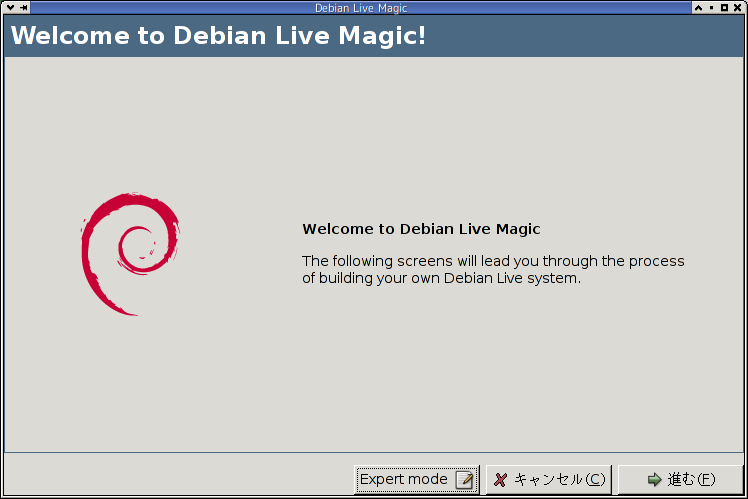
\includegraphics[width=1\hsize]{image200711/live-magic00.png}
 \end{center}
 \caption{live-magic $B5/F02hLL(B}
 \label{live-magic00}
 \end{figure}
\end{multicols}


\subsubsection{$B4pK\%7%9%F%`$NA*Br(B}
$B<!$K4pK\%7%9%F%`$rA*Br$7$^$9!#A*Br2DG=$J%7%9%F%`$O0J2<$NDL$j$G$9!#(B

\begin{multicols}{2}
 \begin{itemize}
 \item Gnome
 \item KDE
 \item XFCE
 \item non-Desktop
 \item $B%7%9%F%`I|5lMQ(B 
 \end{itemize}

 \begin{figure}[H]
 \begin{center}
  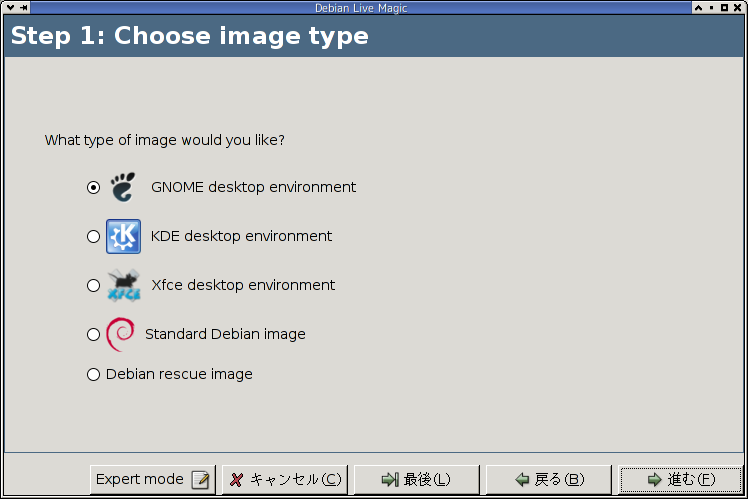
\includegraphics[width=1\hsize]{image200711/live-magic01.png}
 \end{center}
 \caption{live-magic $B4pK\%7%9%F%`$NA*Br(B}
 \label{live-magic01}
 \end{figure}
\end{multicols}

\subsubsection{$B:n@.%$%a!<%8$NA*Br(B}
$B<!$K:n@.$9$k%$%a!<%8$rA*Br$7$^$9!#A*Br2DG=$J%$%a!<%8$O0J2<$NDL$j$G$9!#(B

\begin{multicols}{2}
 \begin{itemize}
 \item CD-ROM $B%$%a!<%8(B
 \item HDD $B%$%a!<%8(B
 \item NFS $B%$%a!<%8(B 
 \end{itemize}

 \begin{figure}[H]
 \begin{center}
  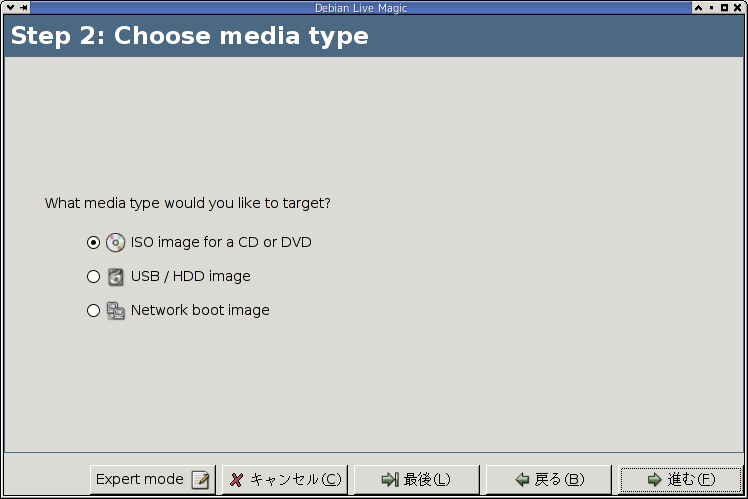
\includegraphics[width=1\hsize]{image200711/live-magic02.png}
 \end{center}
 \caption{live-magic $B:n@.%$%a!<%8$NA*Br(B}
 \label{live-magic02}
 \end{figure}
\end{multicols}

\subsubsection{$B%"!<%-%F%/%A%c$NA*Br(B}
$B<!$KBP>]$N%"!<%-%F%/%A%c$rA*Br$7$^$9!#A*Br2DG=$J%"!<%-%F%/%A%c$O0J2<$NDL$j$G$9!#(B

\begin{multicols}{2}
 \begin{itemize}
 \item i386
 \item powerpc
 \item amd64 
 \end{itemize}

 \begin{figure}[H]
 \begin{center}
  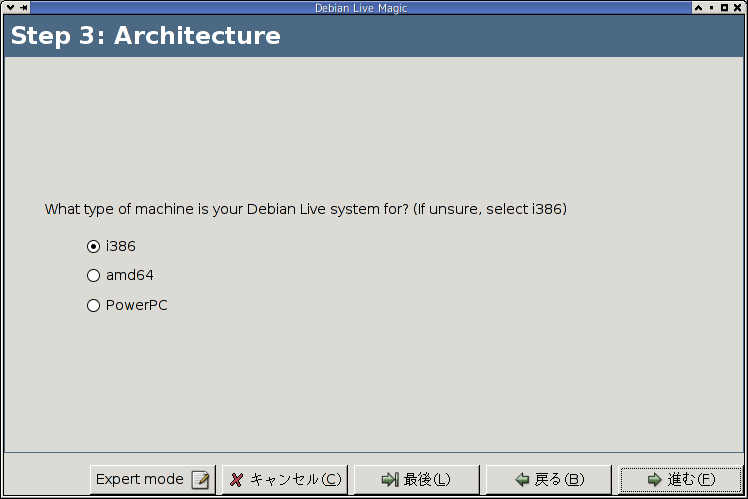
\includegraphics[width=1\hsize]{image200711/live-magic03.png}
 \end{center}
 \caption{live-magic $B%"!<%-%F%/%A%c$NA*Br(B}
 \label{live-magic03}
 \end{figure}
\end{multicols}

\subsubsection{$B%_%i!<%5!<%P!<$NA*Br(B}
\begin{multicols}{2}
 $B<!$K%_%i!<%5!<%P!<$rA*Br$7$^$9!#(B

 \begin{figure}[H]
 \begin{center}
  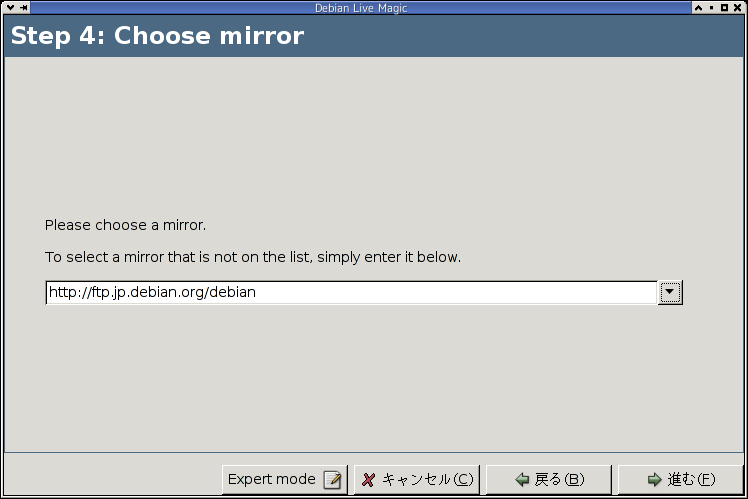
\includegraphics[width=1\hsize]{image200711/live-magic04.png}
 \end{center}
 \caption{live-magic $B%_%i!<%5!<%P!<$NA*Br(B}
 \label{live-magic04}
 \end{figure}
\end{multicols}

\subsubsection{$B%$%a!<%8:n@.<B9T(B}
\begin{multicols}{2}
 $BE,MQ%\%?%s$r2!$9$H!"%$%a!<%8:n@.$r<B9T$7$^$9!#(B

 \begin{figure}[H]
 \begin{center}
  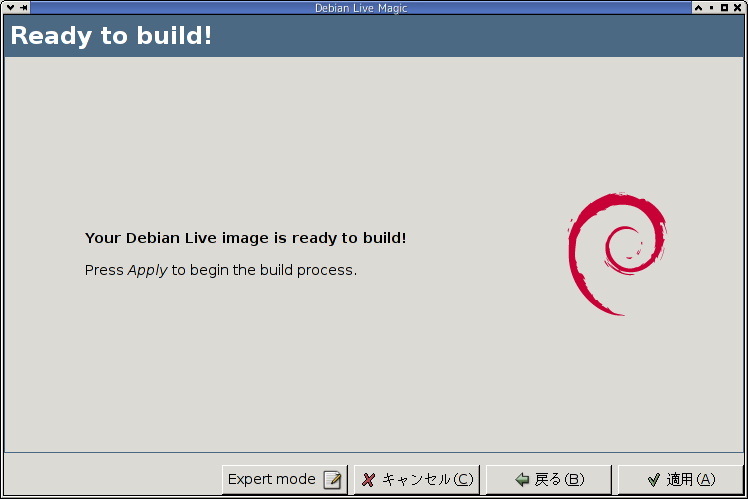
\includegraphics[width=1\hsize]{image200711/live-magic05.png}
 \end{center}
 \caption{live-magic $B%$%a!<%8:n@.<B9T(B}
 \label{live-magic05}
 \end{figure}
\end{multicols}


\subsubsection{root$B%Q%9%o!<%IMW5a(B}

\begin{multicols}{2}
 $B0lHL%f!<%6!<$G<B9T$7$?>l9g!"!!(Broot$B$N%Q%9%o!<%I$rMW5a$5$l$^$9!#(B

 \begin{figure}[H]
 \begin{center}
  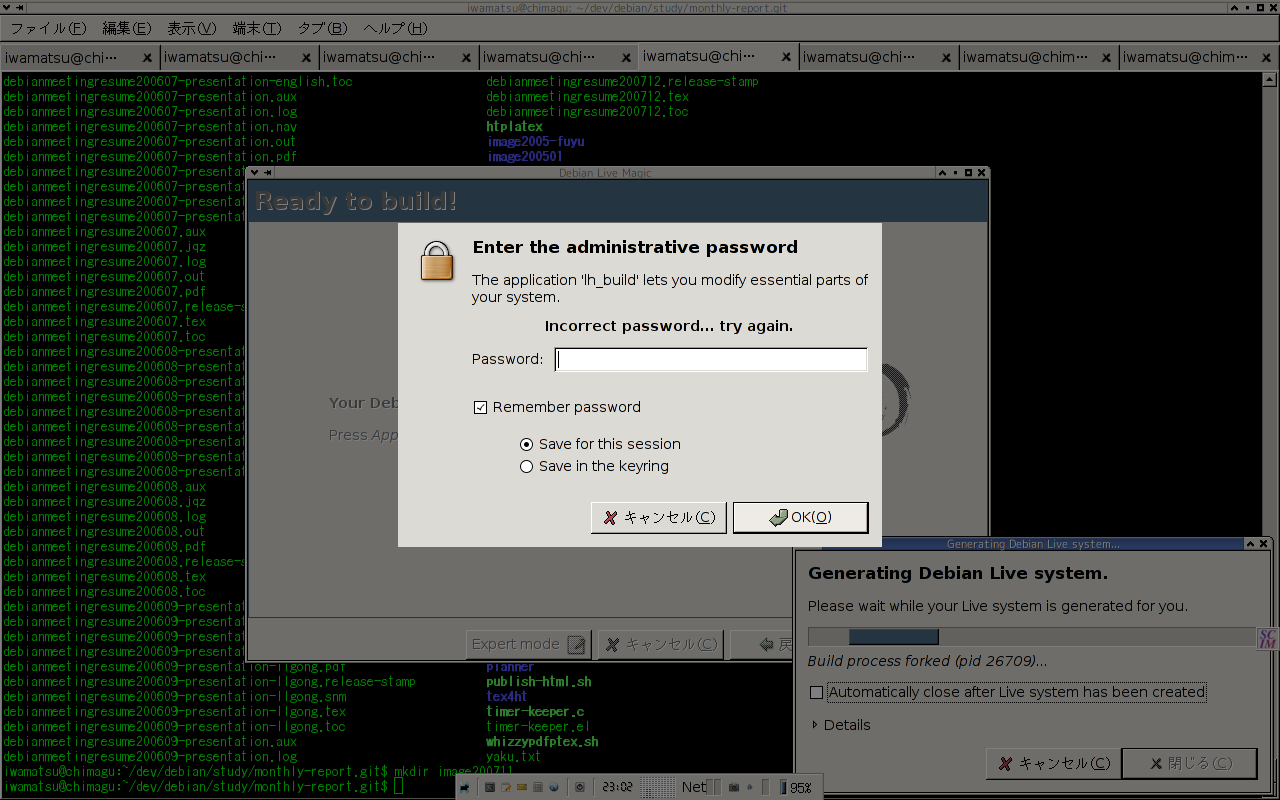
\includegraphics[width=1\hsize]{image200711/live-magic06.png}
 \end{center}
 \caption{live-magic root$B%Q%9%o!<%IMW5a2hLL(B}
 \label{live-magic06}
 \end{figure}
\end{multicols}

\subsubsection{$B:n@.Cf2hLL(B}

\begin{multicols}{2}
 $B%$%a!<%8:n@.Cf$O%W%m%0%l%9%P!<$,I=<($5$l!"ESCf7P2a$r3NG'$9$k$3$H$,$G$-$^$9!#(B

 \begin{figure}[H]
 \begin{center}
  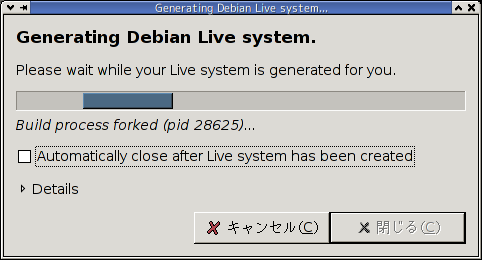
\includegraphics[width=1\hsize]{image200711/live-magic07.png}
 \end{center}
 \caption{live-magic $B:n@.Cf2hLL(B}
 \label{live-magic07}
 \end{figure}
\end{multicols}

\subsubsection{$B%G%P%C%0J}K!(B}
$BF0:n3NG'$d%G%P%C%0$N$?$a$K!"Kh2s:n@.$7$?(B CD/DVD ISO $B%$%a!<%8$r(B $B>F$$$F$$$k$H(B
$B;~4V$b$*6b$b$+$+$j$^$9$N$G!":n@.$7$?(B ISO $B%$%a!<%8$N%G%P%C%0J}K!$K$D$$$F4JC1$K@b(B
$BL@$7$?$$$H;W$$$^$9!#(B

$B%G%P%C%0J}K!$O$$$m$$$m$"$j$^$9$,!"<+J,$O(Bqemu\footnote{http://packages.debian.org/sid/qemu}$B$r;H$C$FF0:n3NG'$7$F$$$^$9!#(B
\begin{commandline}
# apt-get update
# apt-get install qemu
% qemu -cdrom binary.iso
\end{commandline}
qemu $B$r;H$C$?%(%_%e%l!<%7%g%s4D6-$G%G%P%C%0$9$k$3$H$K$h$j!";~4V$d(B CD-R $BBe$N@aLs$K$b$J$j$^$9!#(B
$BB>$NJ}K!$H$7$F$O!"(BVMWare,VirtualPC $B$r;H$C$?%G%P%C%0J}K!$J$I$b9M$($i$l$^$9!#(B

\subsection{live-helper $B$r;H$C$F$_$F(B}
\subsubsection{Live-CD$B$+$i$N%$%s%9%H!<%k$N%5%]!<%H(B}
$B8=>u!"(BLive-CD $B$+$i$N%$%s%9%H!<%k$,%5%]!<%H$5$l$F$$$^$;$s!#(B
HDD$B%$%a!<%8$r:n@.$9$k$3$H$O$G$-$^$9$,!"0lHL%f!<%6!<$K$OI_5o$,9b$$$H9M$($F$$$^$9!#(B
Live-CD $B$,5$$KF~$C$?$J$i!"F0:n$7$F$$$k(B PC $B$K%$%s%9%H!<%k$,MF0W$K$G$-$k$h$&$K$J$l$P(B
$B%f!<%6!<$OA}$($k$N$G$O$J$$$G$7$g$&$+!#(B

\subsubsection{$BF|K\8l4D6-$N%5%]!<%H(B}
live-helper $B$K$O!"$"$kDxEY$N4D6-$r$^$H$a$?$b$N$H$7$F!"(B
packages-selections $B$H$$$&$b$N$,Ds6!$5$l$F$$$^$9!#(B
$B$3$l$KF|K\8l4D6-$b%5%]!<%H$KF~$l$k$3$H$K$h$C$F!"F|K\8lBP1~$N(B Live-CD $B:n@.$,MF0W(B
$B$K$J$k$H;W$$$^$9!#(B

\subsubsection{live-magic $B$NF|K\8l2=(B}
live-helper $B$N%U%m%s%H%(%s%I$G$"$k(B live-magic $B$,1Q8l$N$^$^$J$N$G!"9q:]2=$r$7$?$$(B
$B$H$3$m$G$9!#(B


\subsection{$B$=$NB>$N>pJs(B}
live-helper $B$N>pJs$O0J2<$N%5%$%H$+$iF@$k$3$H$,$G$-$^$9!#(B
\begin{enumerate}
\item live-helper $B8x<0%5%$%H(B \url{http://debian-live.alioth.debian.org/}
\item wiki.debian.org \url{http://wiki.debian.org}

\end{enumerate}

% kansai debian
% ohura-san


\dancersection{20$BJ,$G:n$k(B Debian $B%Q%C%1!<%8(B}{$BBg1:(B $B??(B (Debian Project)}

\subsection{$B$O$8$a$K(B}


\begin{description}
\item[$B%F!<%^(B] $B?M$O2?J,$G(B Debian $B%Q%C%1!<%8$r:n$k$3$H$,$G$-$k$N$+!#(B
  ($B@bL@$r$7$J$,$i(B)
\item[$BBj:`(B] GNU Hello (\url{http://www.gnu.org/software/hello/})
\end{description}


\subsection{$B<j=g(B}

\begin{enumerate}
\item $BI,MW$J%Q%C%1!<%8$N%$%s%9%H!<%k!#(B
  \begin{itemize}
  \item \textbf{build-essential}
  \item $B$=$N%=%U%H%&%'%"$N%S%k%I$KI,MW$J%Q%C%1!<%8!#(B
  \item \textbf{dh-make}$B!"(B\textbf{debhelper}$B!"(B\textbf{devscripts}$B!"(B
      \textbf{fakeroot}$B!"(B\textbf{lintian}/\textbf{linda}
  \end{itemize}
\item $B%Q%C%1!<%8$r:n$j$?$$%=%U%H%&%'%"$N%"!<%+%$%V$rMQ0U$7E83+!#(B
\item \texttt{dh\_make} $B$G%=!<%9%D%j!<$N?w7?$r:n@.!#(B
\item $B$R$H$^$:(B \texttt{debuild} $B$G%Q%C%1!<%8$r:n$C$F$_$k!#(B
\item $B$&$^$/$$$+$J$$>l9g$O!"%m%0$d(B \texttt{./debian/rules} $B%U%!%$%k$r3NG'!#(B
\item $B$&$^$/$G$-$?>l9g$O!"(B\texttt{./debian/} $B0J2<$N%U%!%$%k$r3NG'!#(B
  \begin{itemize}
  \item \texttt{./debian/changelog}: Debian $B%Q%C%1!<%8$N99?7MzNr!#(B
  \item \texttt{./debian/control}: Debian $B%Q%C%1!<%8$N>pJs!#(B
    ($B0MB84X78$d@bL@J8(B)
  \item \texttt{./debian/copyright}: $B%=%U%H%&%'%"$N%i%$%;%s%9$N@bL@!#(B
  \item \texttt{./debian/*.ex}: $BI,MW$K$J$k$+$b$7$l$J$$%U%!%$%k$N?w7?!#(B
    $BI,MW$J$1$l$P$=$N$^$^:o=|!#(B
  \end{itemize}
\item \texttt{lintian} $B%3%^%s%I$N=PNO$r3NG'$7!"=$@5!#(B
\item $B%$%s%9%H!<%k!#(B
\end{enumerate}

\begin{itemize}
\item $B@8@.$5$l$k%U%!%$%k(B
\begin{description}
\item[\ttfamily{}*.orig.tar.gz] $B%*%j%8%J%k$N%=!<%9%"!<%+%$%V!#(B
\item[\ttfamily{}*.diff.gz] $B%*%j%8%J%k$N%=!<%9$H(B Debian $B%=!<%9%Q%C%1!<%8$H$N4V$N:9J,!#(B
\item[\ttfamily{}*.dsc] Debian $B%=!<%9%Q%C%1!<%8$N>pJs!#(B
\item[\ttfamily{}*\_i386.deb] $B%P%$%J%j%Q%C%1!<%8!#(B
\item[\ttfamily{}*\_i386.changes] Debian $B%Q%C%1!<%8$N>pJs$H:G?7$NJQ99MzNr!#(B
\item[\ttfamily{}*\_i386.build] \texttt{debuild} $B$N%m%0!#(B
\end{description}
\end{itemize}

\subsection{$B;29MJ88%(B}

\begin{itemize}
\item $B!VF~Lg(B Debian $B%Q%C%1!<%8!W(B($B$d$^$@$"$-$i(B[$BCx(B]$B!"1-;t(B $BJ8IR(B[$B4F=$(B]) $B5;=QI>O@<R(B
  (ISBN-10: 477412768X)
\item Debian Project $B$N(B Web $B%Z!<%8Fb$N!V(BDebian $B3+H/<T$N%3!<%J!<!W(B
  (\url{http://www.jp.debian.org/devel/})$B!#(B
  $BFC$K!"!V(BDebian $B%]%j%7!<%^%K%e%"%k!W!V%G%Y%m%C%Q!<%:%j%U%!%l%s%9!W(B
  $B!V?75,%a%s%F%J$N$?$a$N%,%$%I!W(B
\end{itemize}

\dancersection{Debian $B%Q%C%1!<%8$N:n$jJ}(B(2) -- debian/rules $B$rFI$`(B --}{$BBg1:(B $B??(B}

\subsection{$B$O$8$a$K(B}

\begin{description}
\item[$B%F!<%^(B] \texttt{debian/rules} $B%U%!%$%k$rFI$s$G$_$k!#(B
\item[$BBj:`(B] \texttt{hello-debhelper} $B%Q%C%1!<%8$N%=!<%9%Q%C%1!<%8!#(B
  \texttt{debhelper} $B$N4JC1$J%5%s%W%k$K$J$C$F$$$k!#(B
\end{description}

\subsection{debian/rules $B$H$O(B}

\begin{itemize}
\item Debian $B%Q%C%1!<%8$r:n$k$?$a$N<jB3$-$r5-=R$7$?%U%!%$%k!#(B
\item makefile $B$K$J$C$F$$$k!#(B
  \begin{itemize}
  \item $B0l9TL\$O(B `\texttt{\#!/usr/bin/make -f}' $B$H$J$C$F$$$J$1$l$P$J$i$J$$!#(B
  \item $B:GDc8B!"(Bclean$B!"(Bbinary$B!"(Bbinary-arch$B!"(Bbinary-indep$B!"(Bbuild $B$N(B
    $B8^$D$N%?!<%2%C%H$r4^$s$G$$$J$1$l$P$J$i$J$$!#(B
  \item $BI,?\$N%?!<%2%C%H0J30$O<+M3$KMxMQ$7$F$$$$!#(B
  \end{itemize}
  \begin{description}
  \item[{\ttfamily{}build}] $B%=!<%9%Q%C%1!<%8$N@_Dj$H%3%s%Q%$%k$r9T$&(B
    $B$?$a$N%?!<%2%C%H(B
  \item[{\ttfamily{}binary$B!"(Bbinary-arch$B!"(Bbinary-indep}]
    $B%P%$%J%j%Q%C%1!<%8$r:n$k$?$a$N%?!<%2%C%H!#(B
    binary-arch $B$O!"%"!<%-%F%/%A%c$K0MB8$7$?%Q%C%1!<%8!"(B
    binary-indep $B$O!"%"!<%-%F%/%A%c$K0MB8$7$J$$%Q%C%1!<%8$r:n$k!#(B
    binary $B$O$=$NN>J}$N%Q%C%1!<%8$r:n$k!#(B
  \item[{\ttfamily{}clean}] 
    $B%P%$%J%j%Q%C%1!<%8$N:n@.8e!"%=!<%9%Q%C%1!<%8$r85$N>uBV$KLa$9$?$a$N(B
    $B%?!<%2%C%H!#(B
  \item[{\ttfamily{}install}]
    $B%=!<%9%Q%C%1!<%8$N%3%s%Q%$%k8e!"5,Dj$N0LCV$K%U%!%$%k$r(B
    $BCV$/$?$a$N%?!<%2%C%H!#(B
    \texttt{build} $B%?!<%2%C%H$G:n@.$5$l$?%U%!%$%k$O0lC6!"(B
    \texttt{debian/\$(package)/} $B0J2<$K%$%s%9%H!<%k$5$l$k!#(B
  \item[{\ttfamily{}configure}] $B%=!<%9%Q%C%1!<%8$N@_Dj$r9T$&$?$a$N(B
    $B%?!<%2%C%H!#(B
  \item[{\ttfamily{}get-orig-source}] $B%*%j%8%J%k$N%=!<%9%Q%C%1!<%8$r(B
    $B<hF@$9$k$?$a$N%?!<%2%C%H!#(B
    $B$"$^$jCN$i$l$F$$$J$$!#(B
  \end{description}
\item $B$=$l$>$l$N%?!<%2%C%H$r<B9T$9$k$?$a$N<j=u$1$r$9$k(B
  \texttt{debhelper} $B$H$$$&0lO"$N%9%/%j%W%H$,$"$k!#(B
  \begin{itemize}
  \item $BA4$F(B \texttt{dh\_} $B$G;O$^$kL>A0$N(B perl $B%9%/%j%W%H!#(B
  \item \texttt{debhelper(7)} $B$K%9%/%j%W%H$N0lMw$,$"$k!#(B
  \end{itemize}
  \begin{description}
  \item[\ttfamily{}dh\_clean] $B%=!<%9%Q%C%1!<%8$NCf$N$$$i$J$$%U%!%$%k$r(B
    $B:o=|$9$k!#(B
  \item[\ttfamily{}dh\_installdirs] \texttt{debian/\$(package)/} $B0J2<$K(B
    $BI,MW$J%G%#%l%/%H%j$r:n@.$9$k!#(B
  \item[\ttfamily{}dh\_installdocs$B!"(Bdh\_installchangelog]
    \texttt{usr/share/doc/} $B0J2<$K%I%-%e%a%s%H$d(B changelog $B$r(B
    $B%$%s%9%H!<%k!#(B
  \end{description}
  $B$J$I$J$I!#(B
\end{itemize}


\subsection{$B;29MJ88%(B}

\begin{itemize}
\item Debian Policy (\url{http://www.jp.debian.org/doc/debian-policy/})
  $B!V(B4.9 Main building script: debian/rules$B!W(B
\end{itemize}

\dancersection{Debian $B%Q%C%1!<%8$N:n$jJ}(B(3) -- dpatch $B$N;H$$J}(B --}{$BBg1:(B $B??(B}
\subsection{$B$O$8$a$K(B}
\begin{description}
\item[$B%F!<%^(B] Debian $B%Q%C%1!<%8$N(B patch $B4IM}%7%9%F%`$G$"$k(B dpatch $B$r(B
  $B;H$C$F$_$k!#(B
\item[$BAG:`(B] \texttt{hello-debhelper} $B%Q%C%1!<%8$N%=!<%9%Q%C%1!<%8!#(B
  $B%a%C%;!<%8$rJQ99$9$k(B patch $B$r:n$C$F$_$k!#(B
\end{description}


\subsection{Debian $B%Q%C%1!<%8$H(B patch}

\begin{itemize}
\item Debian $B$N%=!<%9%Q%C%1!<%8$O;0$D$N%U%!%$%k$+$i=PMh$F$$$k!#(B
  \begin{description}
  \item[\ttfamily{}*.orig.tar.gz] $B%*%j%8%J%k$N%=!<%9%"!<%+%$%V!#(B
  \item[\ttfamily{}*.diff.gz] $B%*%j%8%J%k$N%=!<%9$H(B
    Debian $B%=!<%9%Q%C%1!<%8$H$N4V$N:9J,!#(B
  \item[\ttfamily{}*.dsc] Debian $B%=!<%9%Q%C%1!<%8$N>pJs!#(B
  \end{description}
\item debian/ $B0J2<$N%U%!%$%k$b4^$a$F!"%*%j%8%J%k$H$N:9J,$OA4$F(B
  .diff.gz $B$K$^$H$a$i$l$k$N$G!"(B
  Debian $BB&$G(B patch $B$rJ#?t$"$F$F$$$k>l9g$O4IM}$,LLE]!#(B
\item dpatch $B$r;H$&$H!"(Bpatch $B$rJ,3d$7$F4IM}$9$k$3$H$,$G$-$k!#(B
  $B%*%j%8%J%k$,99?7$5$l$?;~$NDI?o$b4JC1!#(B
\item debian/patches/ $B0J2<$G(B patch $B$r$^$H$a$F4IM}!#(B
\item $B0\9T$K(B .orig.tar.gz $B$N=$@5$OITMW!#(B
\end{itemize}

\subsection{dpatch $B$N;H$$J}(B}

\begin{itemize}
\item debian/rules $B$N=$@5(B
  \begin{itemize}
  \item $BKAF,$K(B \texttt{include /usr/share/dpatch/dpatch.make} $B$rDI2C!#(B
  \item \texttt{build} $B%?!<%2%C%H$G(B \texttt{patch} $B%?!<%2%C%H$,!"(B
    \texttt{clean} $B%?!<%2%C%H$G(B
    \texttt{unpatch} $B%?!<%2%C%H$,<B9T$5$l$k$h$&$KJQ99$9$k!#(B
  \end{itemize}
  \begin{screen}[5]
    \#!/usr/bin/make -f \\
    \hspace{4em}\ldots \\
    include /usr/share/dpatch/dpatch.make \\
    clean: unpatch \\
    \hspace{4em}\ldots \\
    install: build \\
    \hspace{4em}\ldots \\
    build: patch \\
    \hspace{4em}\ldots
  \end{screen}
\item debian/control $B$N(B Build-Depends: $B$K(B dpatch $B$rDI2C!#(B
\item \textsf{dpatch-convert-diffgz} $B$r;H$&$H(B \texttt{.diff.gz} $B$NCf$N(B
  debian/* $B0J30$N%U%!%$%k$KBP$9$k(B patch $B$rCj=P$G$-$k!#(B
\item \textsf{dpatch-edit-patch} $B$G(B patch $B$r:n@.!#(B
  \begin{screen}[5]
    \$ dpatch-edit-patch 01\_hello\_japan \\
    ( \ldots $B<+F0E*$K(B /tmp $B0J2<$K%3%T!<$,:n$i$l!"?7$7$$%7%'%k$,5/F0$9$k!#(B) \\
    ( \ldots $B%=!<%9%D%j!<$r=$@5!#(B) \\
    \$ exit \\
    \$ 
    ( \ldots debian/patches/ $B0J2<$K(B patch $B$,$G$-$k!#(B)
  \end{screen}
  $B4{B8$N(B patch $B$NJT=8$b$G$-$k!#(B
\item $B$G$-$?(B patch ($B>eNc$G$O!"(Bdebian/patches/01\_hello\_japan.dpatch) $B$K(B
  $BE,Ev$J%3%a%s%H$r=q$$$F$*$/!#(B
\item patch $B$r(B debian/patches/00list $B$KDI2C!#(B
  $B%U%!%$%kL>$N(B .dpatch $B$r=|$$$?J8;zNs$rDI2C!#(B
\item patch $B$,$-$A$s$HE,MQ$G$-$k$+$I$&$+$O!"(B
  \textsf{fakeroot ./debian/rules patch}$B!"(B
  \textsf{fakeroot ./debian/rules unpatch} $B$G3NG'$G$-$k!#(B
\item \textsf{dpatch-list-patch} $B$G(B patch $B$N0lMw$r3NG'$G$-$k!#(B
\end{itemize}

\subsection{$BN`;w$N%7%9%F%`(B}

\begin{itemize}
\item dbs: $B%*%j%8%J%k$N%=!<%9$,(B .tar.gz $B$N7A$G$=$N$^$^(B .orig.tar.gz $B$K(B
  $B4^$^$l$k!#0\9T$K$O!"(B.orig.tar.gz $B$N=$@5$,I,MW!#(B
\item quilt
\end{itemize}

\subsection{$B;29MJ88%(B}

\begin{itemize}
\item dpatch$B$NMxMQJ}K!(B
  (\url{http://www.netfort.gr.jp/~dancer/column/dpatch.html.ja})
\item dpatch(1), dpatch.make(7),
  /usr/share/doc/dpatch/examples/rules/rules.new.dh.gz
\item $B!VF~Lg(B Debian $B%Q%C%1!<%8!W(B($B$d$^$@$"$-$i(B[$BCx(B]$B!"1-;t(B $BJ8IR(B[$B4F=$(B]) $B5;=QI>O@<R(B
  (ISBN-10: 477412768X)
\end{itemize}


\dancersection{Debian $B%Q%C%1!<%8$N:n$jJ}(B(4) -- $B%i%$%V%i%jJT(B --}{$BBg1:(B $B??(B}
\subsection{$B$O$8$a$K(B}

\begin{description}
\item[$B%F!<%^(B] $B%i%$%V%i%j$N(B Debian $B%Q%C%1!<%8:n@.$r<B1i$7$F$_$k!#(B
  $BIaDL$N%Q%C%1!<%8$h$j$b>/$7J#;(!#(B
\item[$BAG:`(B] \texttt{libhello} (``Hello, library world.'' $B$HI=<($9$k(B
  $B4X?t(B hello $B$rDs6!$9$k%i%$%V%i%j(B)
\end{description}

\subsection{$B4pK\E*$J<j=g(B}

\begin{enumerate}
\item $BI,MW$J%Q%C%1!<%8$N%$%s%9%H!<%k!#(B
  \begin{itemize}
  \item \textbf{build-essential}
  \item $B$=$N%=%U%H%&%'%"$N%S%k%I$KI,MW$J%Q%C%1!<%8!#(B
  \item \textbf{dh-make}$B!"(B\textbf{debhelper}$B!"(B\textbf{devscripts}$B!"(B
      \textbf{fakeroot}$B!"(B\textbf{lintian}/\textbf{linda}
  \end{itemize}
\item $B%Q%C%1!<%8$r:n$j$?$$%=%U%H%&%'%"$N%"!<%+%$%V$rMQ0U$7E83+!#(B
\item \texttt{dh\_make} $B$G%=!<%9%D%j!<$N?w7?$r:n@.!#(B
\item $B$R$H$^$:(B \texttt{debuild} $B$G%Q%C%1!<%8$r:n$C$F$_$k!#(B
\item $B$&$^$/$$$+$J$$>l9g$O!"%m%0$d(B \texttt{debian/rules} $B%U%!%$%k$r3NG'!#(B
\item $B$&$^$/$G$-$?>l9g$O!"(Blintian $B$N=PNO$d(B
  \texttt{debian/} $B0J2<$N%U%!%$%k$r3NG'$7!"$5$i$K=$@5!#(B
\end{enumerate}


\subsection{$B%i%$%V%i%j%Q%C%1!<%8$N:n$jJ}(B}


\begin{itemize}
\item $B%i%$%V%i%j%Q%C%1!<%8$O!"6&M-%i%$%V%i%jK\BN$,4^$^$l$k(B
  $B%Q%C%1!<%8(B (\textbf{libhello0}) $B$H3+H/MQ$N%U%!%$%k$,4^$^$l$k(B
  $B%Q%C%1!<%8(B (\textbf{libhello-dev}) $B$KJ,$+$l$F$$$k!#(B
\item $B%i%$%V%i%j$N>l9g$b!"(B\texttt{dh\_make} $B$G?w7?$r:n$k$3$H$,$G$-$k$,(B
  $B$=$N$^$^$G$O%Q%C%1!<%8$,$G$-$J$$!#(B
\item \texttt{debian/control} $B$N=$@5(B
  \begin{itemize}
  \item \texttt{dh\_make} $B$N;X<(DL$j!"(B`libhelloBROKEN' $B$H$J$C$F$$$k(B
    $BItJ,$r=$@5!#(B
    $B$3$N>l9g$O!"(B`libhello0' $B$K$9$k!#(B
  \end{itemize}
\item \texttt{debian/rules} $B$N=$@5(B
  \begin{itemize}
  \item `\$(MAKE) distclean' $B$N9T$r(B
    `[ ! -f Makefile ] $||$ \$(MAKE) distclean' $B$KJQ99!#(B
  \item \texttt{dh\_install} $B$K(B `--sourcedir=debian/tmp' $B$H$$$&%*%W%7%g%s$r(B
    $BIU$1$kI,MW$,$"$k(B
    \footnote{$B$+$D$F$O(B \texttt{dh\_movefiles} $B$H$$$&$b$N$,$"$C$?$,!"8=:_$O(B
      $B;H$o$l$F$$$J$$!#(B}$B!#(B
  \item \texttt{dh\_makeshlibs} $B$rM-8z$K$9$k!#(B-V $B%*%W%7%g%s$rIU$1$k!#(B
    $BM-8z$K$9$k$H!"E,@Z$J(B \texttt{postinst}/\texttt{postrm} $B%9%/%j%W%H$,(B
    $BMQ0U$5$l$k!#(B(install $B;~$H(B remove $B;~$K(B \texttt{ldconfig} $B$,(B
    $B<B9T$5$l$k!#(B)
  \end{itemize}
\item $B$=$NB>(B
  \begin{itemize}
  \item \texttt{libhello1.dirs} $B$H(B \texttt{libhello1.install} $B$r(B
    \texttt{libhello0} $B$KL>A0$rJQ$($k!#(B
  \item \texttt{libhello-dev.install} $B$+$i(B \textbf{pkg-config} $B4X78$r:o=|!#(B
  \item $BITMW$J(B \texttt{debian/*.ex} $B$r:o=|!#(B
  \end{itemize}
\end{itemize}


\subsection{$B6&M-%i%$%V%i%j$NL>A0(B}

\begin{itemize}
\item $B6&M-%i%$%V%i%j$O!";0$D$NL>A0$r;}$D!#(B
  \begin{description}
  \item[soname] (\texttt{/usr/lib/libhello.so.0}):
    $B<B9T%U%!%$%k$,;2>H$9$kL>A0!#%i%$%V%i%j$N%$%s%?!<%U%'%$%9$,JQ99$5$l$k$H(B
    $BKvHx$N?t;z$,JQ$o$k!#(B
    Debian $B$G$O$3$N?t;z$r%Q%C%1!<%8L>$KIU2C$9$k!#(B
  \item[real name] (\texttt{/usr/lib/libhello.so.0.0.0}):
    $B%i%$%V%i%j$N<BBN!#(Bsoname $B$O$3$N%U%!%$%k$X$N%7%s%\%j%C%/%j%s%/$K$J$C$F$$$k!#(B
  \item[linker name] (\texttt{/usr/lib/libhello.so}):
    $B%i%$%V%i%j$rMxMQ$9$k%W%m%0%i%`$r%3%s%Q%$%k$9$k$H$-$K;2>H$9$kL>A0!#(B
  \end{description}
\end{itemize}

\subsection{$B;29MJ88%(B}

\begin{itemize}
\item \url{http://www.linux.or.jp/JF/JFdocs/Program-Library-HOWTO/}
  $B!V(BProgram Library HOWTO$B!W(B(JF)
\item \url{http://www.netfort.gr.jp/~dancer/column/libpkg-guide/libpkg-guide.html}
  $B!V(BDebian Library Packaging guide$B!W(B
\end{itemize}


\subsection{$B%5%s%W%k(B}


\begin{itembox}{\texttt{libhello.c}}
\begin{verbatim}
#include <stdio.h>

void hello(void) {
        printf("Hello, library world.\n");
}
\end{verbatim}
\end{itembox}

\begin{itembox}{\texttt{libhello.h}}
\begin{verbatim}
void hello(void);
\end{verbatim}
\end{itembox}

\begin{itembox}{\texttt{demo\_use.c}}
\begin{verbatim}
#include "libhello.h"

int main(void) {
        hello();
        return 0;
}
\end{verbatim}
\end{itembox}

% FIXME: $BE>5-$9$k$3$H(B


\newpage
\dancersection{Debian Weekly News trivia quiz}{$B>e@n(B $B=c0l(B}

$B$H$3$m$G!"(BDebian Weekly News (DWN)$B$OFI$s$G$$$^$9$+!)(B
Debian $B3&7($G$*$-$F$$$k$3$H$K$D$$$F=q$$$F$$$k(BDebian Weekly News$B!#(B
$BKh2sFI$s$G$$$k$H$$$m$$$m$HJ,$+$C$FMh$^$9$,!"0l?M$GFI$s$G$$$F$b!"2r@b$,>/(B
$B$J$$$N$G!"(B
$B0UL#$,$o$+$i$J$$$H$3$m$b$"$k$+$bCN$l$^$;$s!#$_$s$J$G(BDWN$B$rFI$s$G$_$^$7$g$&!#(B

$BL!A3$HFI$`$@$1$G$O$*$b$7$m$/$J$$$N$G!"(BDWN$B$N5-;v$+$i=PBj$7$?0J2<$N<ALd$K$3$?$($F$_$F$/$@$5$$!#(B
$B8e$GFbMF$O2r@b$7$^$9!#(B

\subsection{2007$BG/(B6$B9f(B}
\url{http://www.debian.org/News/weekly/2007/06/}
$B$K$"$k(B7$B7n(B3$BF|HG$G$9!#(B

\santaku
{Andr\'e Luiz Rodrigues Ferreira $B$,@k8@$7$?$N$O$I$N%&%'%V%5%$%H$+(B}
{Debian art}
{Debian pop}
{Debian tart}
{A}

\santaku
{J\"ulich $B$G9T$o$l$?2q5D$G(B lenny $B$N%j%j!<%9%W%m%;%9$K$D$$$F2?$r$9$k$3$H$,7h$^$C$?$+(B}
{$BHkL)$N%W%m%;%9$K$N$C$H$j!":#8e%j%j!<%9$,$I$&$J$C$F$$$k$+$OHs8x3+$K$9$k(B}
{$BKh7n$+Fs%v7n$K0l2s$N:G=*=5$K%j%j!<%9>u67$K$D$$$F$N%a!<%k$r=P$9(B}
{$B0BA4J]>c$N$?$a:#8e$O(B Debian Developer$B$G$J$$$H%j%j!<%9$N>u67$,$o$+$i$J$$$h$&$K$9$k(B}
{B}

\santaku
{Lucas Nussbaum $B$OKh7n2?$r$9$k$HH/I=$7$?$+(B}
{$B?<9o$JLdBj$N$"$k%Q%C%1!<%8$r=gHV$K$N$C$H$k(B}
{$B?<9o$JLdBj$N$"$k%Q%C%1!<%8$r4IM}$7$F$$$k?M$KH3%2!<%`$r$5$;$k(B}
{$B?<9o$JLdBj$N$"$k%Q%C%1!<%8$K$D$$$FDLCN$9$k%a!<%k$r<+F0$GAwIU(B}
{C}

\santaku
{Alexander Wirt $B$O2?$rH/I=$7$?$+(B}
{backports.org $B$,(B sid $B$KBP1~(B}
{backports.org $B$,(B lenny $B$KBP1~(B}
{backports.org $B$,(B etch $B$KBP1~(B}
{C}

\santaku
{Martin Michlmyr $B$,D)@o$7$F$$$k$N$O2?$+(B}
{Debian $B$r(B gcc 4.2$B$G%S%k%I$G$-$k$h$&$K$9$k(B}
{Debian $B$rA4It(B C++ $B$K$*$-$+$($k(B}
{Debian $B$rA4It(B ruby $B$K$*$-$+$($k(B}
{A}

% 2007/08
\subsection{$BLdBj(B}
$B:#2s$N=PBjHO0O$O(B\url{http://www.debian.org/vote/2007/vote_003} $B$K$"$kEjI<(B
$B7k2L$H!"(B\url{http://lists.debian.org/debian-devel-announce/} $B$K$"$k:G6a$N(B
$B%"%J%&%s%9J8=q$G$9!#(B

\santaku{Debian Maintainers $B$NDs0F$O2?$r$9$k$b$N$+(B}
{$B5$$KF~$i$J$$(B Debian Developer $B$rEjI<$K$h$jDIJ|$9$k(B}
{Debian Developer $B$h$j@)8B$5$l$?8"8B$r$b$D(B Debian Maintainers $B$rDj5A$9$k(B}
{Debian Developer $B$NIJ<A$r2~A1$9$k(B}
{B}

\santaku{
Bits from the DPL: FTP assistants, DM, APT, sharing patches
$B$G(B Sam Hocever $B$,<gD%$7$?$N$O(B
}
{$B%Q%C%A$r6&M-$7$h$&(B}
{$B$b$&2qD9$H$7$F$N;E;v$O=*$o$C$?(B}
{Debian $B$H$7$F$O(B Ubuntu $B$N]SLG$,L\I8(B}
{A}

\santaku{
apt-get install $B$N;EAH$_$GBg$-$JJQ2=$,H/@8$7$?$N$O2?$+(B
}
{Suggests  $B$r%G%U%)%k%H$G%$%s%9%H!<%k$9$k$h$&$K$J$C$?(B}
{Recommends $B$r%G%U%)%k%H$G%$%s%9%H!<%k$9$k$h$&$K$J$C$?(B}
{Depends $B$rL5;k$9$k$h$&$K$J$C$?(B}
{B}

\santaku{lenny $B$N%j%j!<%9%4!<%k$KF~$C$F$$$k$N$O$I$l$+(B}
{Debian $B$N;T>l%7%'%"(B40\% $B0J>e$N3MF@(B}
{debian/rules $B$,9q:]2=BP1~(B}
{debian/changelog $B$H(B debian/control $B$O(B UTF-8}
{C}

\santaku{sparc32 $B$K$J$K$,$*$-$?$+(B}
{$B<!$N%j%j!<%9$G$O%5%]!<%H$5$l$J$/$J$k(B}
{$B5^$K%f!<%6$,A}$($?$N$G3+H/<T$rJg=8$7$F$$$k(B}
{arm $B$H%P%$%J%j8_49$K$J$C$?(B}
{B}

% 2007/09
\subsection{$BLdBj(B}
$B:#2s$N=PBjHO0O$O(B\url{debian-devel@lists.deban.org} $B$KEj9F$5$l$?FbMF$+$i$G$9!#(B

\santaku
{Albert Einstein $B$,:n$C$?(B Debian $B%Y!<%9$N%G%#%9%H%j%S%e!<%7%g%s$O2?$+(B}
{ice linux}
{fantasy linux}
{fire linux}
{A}

\santaku
{$B$=$7$F$3$N(BAlbert Einstein $B$,(B debian-devel $B$G<ALd$7$?FbMF$O2?$G$7$g$&(B}
{$B$J$<(B Internet Explorer $B$,(B Debian $B$K$J$$$N$G$9$+!#(B}
{$B$J$<(B Opera $B$,(B Debian $B$K$J$$$N$G$9$+!#(B}
{$B$J$<(B Safari $B$,(B Debian $B$K$J$$$N$G$9$+!#(B}
{B}

\santaku
{Luk Claes $B$,(B RC$B%P%0$K$D$$$FDs0F$7$?$N$O$I$N$h$&$JFbMF$+(B}
{RC$B%P%0$,=P$?%Q%C%1!<%8$N%a%s%F%J$X$N%Z%J%k%F%#$r9M$($kDs0F(B}
{RC$B%P%0$N(B 0-day NMU $B$K$D$$$F$NDs0F(B}
{RC$B%P%0$r$$$+$K$7$FL5;k$9$k$+!"$H$$$&(B HowTo.}
{B}

\santaku
{packages.debian.org$B$K$$$m$$$m?75!G=$,DI2C$5$l$^$7$?!#$I$N$h$&$J5!G=$,DI2C$5$l$^$7$?$+(B}
{$B%a!<%k%U%)%o!<%I5!G=(B}
{$B%+%k%^IU2C5!G=(B}
{Web$B$+$i%Q%C%1!<%8>h$C<h$j5!G=(B}
{A}


% 2007/10
% OSC $B$N$?$a!"$J$7!#(B
% 2007/11
\subsection{$BLdBj(B}
$B:#2s$N=PBjHO0O$O(B\url{debian-devel-announce@lists.deban.org} $B$KEj9F$5$l$?FbMF$+$i$G$9!#(B

 \santaku
 {10/4 $B$K%"%J%&%s%9$,$"$C$?(B alioth $B$N%5!<%S%9$KDI2C$5$l$?$b$N$O!)(B}
 {VSS$B%5%]!<%H(B}
 {darcs$B%5%]!<%H(B}
 {p4$B%5%]!<%H(B}
 {B}

 \santaku
 {DebianGis$B%A!<%`$O2?$r$9$k%A!<%`$+!)(B}
 {Gis$B$N%Q%C%1!<%8$N%a%s%F%J%s%9(B}
 {Debian$B$r(BGis$B$G$N$C$H$k%W%m%8%'%/%H(B}
 {$B?M4V4X78$r%.%9%.%9$7$F$_$k(B}
 {A}

 \santaku
 {testing security $B$N%a!<%k$N;EAH$_$G2?$,$+$o$C$?$+(B}
 {unstable $B$+$i(B testing $B$X$N%^%$%0%l!<%7%g%s$G%;%-%e%j%F%#!<%P%0$,=$@5$5(B
 $B$l$F$b%"%J%&%s%9$5$l$k$h$&$K$7$?(B}
 {$B:rG/EY(B Debian testing security team $B$,(BCVE$B$r(B5500$B$b=hM}$7$?$3$H$,<+K}$G$-$k$h$&$K$J$C$?(B}
 {SMTP$B%W%m%H%3%k$N%O%s%I%7%'!<%/$,JQ$o$C$?(B}
 {A}


 \santaku
 {Debconf8 $B$NF|Dx$O(B}
 {5$B7n(B1$BF|$+$i(B5$B7n(B10$BF|(B}
 {8$B7n(B2$BF|$+$i(B8$B7n(B17$BF|(B}
 {12$B7n(B24$BF|$+$i(B1$B7n(B1$BF|(B}
 {B}

 \santaku
 {http://security-tracker.debian.net/tracker/ $B$G2?$,8+$l$k$+(B}
 {$B<j85$N%^%7%s$,@H<e2=$I$&$+$N;n83(B}
 {$B%;%-%e%j%F%#!<$K$D$$$F$NF~Lg(B}
 {$B%;%-%e%j%F%#!<%P%0$N8=:_$N>uBV(B}
 {C}

 \santaku
 {Debian System Administrator $B$H$7$F?7$7$/G$L?$5$l$?$N$OC/$+(B}
 {Sven Luther}
 {Phil Hands}
 {Peter Palfrader}
 {C}

 \santaku
 {ries.debian.org (ftp-master) $B$O$I$l$/$i$$Dd;_$7$F$$$?$+(B}
 {11$B7n(B5$BF|$+$i(B11$B7n(B12$BF|(B}
 {11$B7n(B5$BF|$+$i(B11$B7n(B30$BF|(B}
 {11$B7n(B1$BF|$+$i(B11$B7n(B5$BF|(B}
 {A}

\dancersection{Debian Weekly News $BLdBj2sEz(B}{$B>e@n(B $B=c0l(B}

\begin{multicols}{2}
 Debian Weekly News $B$NLdBj2sEz$G$9!#(B
 $B$"$J$?$O2?Ld$o$+$j$^$7$?$+!)(B
 \\
 %$B2sEz$O(Bdebianmeetingresume2007-fuyu.jqz$B$H$$$&%U%!%$%k$K@8@.$5$l$k$N$G!"(B
 %$B$=$l$r<jF0$G%3%T%Z$7$F;H$&!#(B
 % $B$3$3$+$i%3%T%Z(B
 % FIXME $BLdBj$,A4It$O$$$C$?$i%3%T%Z$9$k$3$H(B
 %(progn (next-line 1)(insert-file "debianmeetingresume2007-fuyu.jqz") )

\end{multicols}


\printindex

\cleartooddpage

\vspace*{15cm}
{\color{dancerlightblue}\rule{\hsize}{1mm}}
\vspace{2mm}

\includegraphics[width=2cm]{image200502/openlogo-nd.eps}
\noindent \Large \bf $B$"$s$I$-$e$a$s$F$C$I(B $B$G$S$"$s(B 2007$BG/E_9f(B\\ \\
% FIXME $B3+:EF|$,$o$+$C$?$i99?7$9$k$3$H(B
\noindent \normalfont 2007$BG/(B12$B7n(BXX$BF|(B \hspace{5mm}  $B=iHGBh(B1$B:~H/9T(B\\
\noindent \normalfont $BEl5~%(%j%"(B Debian $BJY6/2q(B $B!JJT=8!&0u:~!&H/9T!K(B\\
{\color{dancerdarkblue}\rule{\hsize}{1mm}}

\end{document}

;;; Local Variables: ***
;;; outline-regexp: "\\([ 	]*\\\\\\(documentstyle\\|documentclass\\|dancersection\\)\\*?[ 	]*[[{]\\|[%]+\\)" ***
;;; End: ***
